% =============================================================
% NutriTrack — Rapport Final de Certification
% Expert en Infrastructures de Donnees Massives (RNCP37638)
% =============================================================
\documentclass[a4paper,11pt,oneside,openany]{report}

% ---- Encodage et langue ----
\usepackage[utf8]{inputenc}
\usepackage[T1]{fontenc}
\usepackage[french]{babel}
\usepackage{lmodern}

% ---- Mise en page ----
\usepackage[top=2.5cm, bottom=2.5cm, left=3cm, right=2.5cm]{geometry}
\usepackage{setspace}
\onehalfspacing
\usepackage{parskip}
\setlength{\parindent}{0pt}

% ---- En-tetes et pieds de page ----
\usepackage{fancyhdr}
\pagestyle{fancy}
\fancyhf{}
\fancyhead[L]{\small\nouppercase{\leftmark}}
\fancyhead[R]{\small\thepage}
\fancyfoot[C]{}
\renewcommand{\headrulewidth}{0.4pt}
\renewcommand{\footrulewidth}{0pt}
\setlength{\headheight}{14pt}
% Supprimer le numero de section du rightmark pour eviter le chevauchement
\renewcommand{\chaptermark}[1]{\markboth{\thechapter.\ #1}{}}
\renewcommand{\sectionmark}[1]{}

% ---- Graphiques et couleurs ----
\usepackage{graphicx}
\usepackage{xcolor}
\usepackage{colortbl}
\usepackage{tikz}
\usetikzlibrary{
  positioning, arrows.meta, shapes.geometric, shapes.multipart,
  calc, fit, backgrounds, decorations.pathreplacing, chains,
  matrix, shadows, patterns, babel
}

% ---- Couleurs NutriTrack ----
\definecolor{ntgreen}{HTML}{2E7D32}
\definecolor{ntdarkgreen}{HTML}{1B5E20}
\definecolor{ntlightgreen}{HTML}{A5D6A7}
% Couleurs des grilles d'entretien
\definecolor{producerhead}{HTML}{F9A825}  % Jaune — en-tete grille producteur
\definecolor{producerbody}{HTML}{FFF8E1}  % Jaune clair — lignes producteur
\definecolor{consumerhead}{HTML}{827717}  % Olive — en-tete grille consommateur
\definecolor{consumerbody}{HTML}{F0F4C3}  % Olive clair — lignes consommateur
\definecolor{ntblue}{HTML}{1565C0}
\definecolor{ntlightblue}{HTML}{90CAF9}
\definecolor{ntorange}{HTML}{EF6C00}
\definecolor{ntred}{HTML}{C62828}
\definecolor{ntpurple}{HTML}{6A1B9A}
\definecolor{ntlightpurple}{HTML}{CE93D8}
\definecolor{ntgold}{HTML}{F9A825}
\definecolor{ntgray}{HTML}{616161}
\definecolor{ntlightgray}{HTML}{E0E0E0}
% Nutri-Score
\definecolor{nsA}{HTML}{038141}
\definecolor{nsB}{HTML}{85BB2F}
\definecolor{nsC}{HTML}{FECB02}
\definecolor{nsD}{HTML}{EE8100}
\definecolor{nsE}{HTML}{E63E11}
% Medallion
\definecolor{bronze}{HTML}{CD7F32}
\definecolor{silver}{HTML}{C0C0C0}
\definecolor{gold}{HTML}{FFD700}

% ---- Tableaux ----
\usepackage{booktabs}
\usepackage{tabularx}
\usepackage{multirow}
\usepackage{longtable}
\usepackage{array}
\newcolumntype{L}[1]{>{\raggedright\arraybackslash}p{#1}}
\newcolumntype{C}[1]{>{\centering\arraybackslash}p{#1}}

% ---- Code source ----
\usepackage{listings}
\lstset{
  basicstyle=\ttfamily\footnotesize,
  backgroundcolor=\color{ntlightgray!30},
  frame=single,
  framerule=0.5pt,
  rulecolor=\color{ntgray},
  breaklines=true,
  breakatwhitespace=true,
  numbers=left,
  numberstyle=\tiny\color{ntgray},
  numbersep=8pt,
  tabsize=4,
  showstringspaces=false,
  captionpos=b,
  keywordstyle=\color{ntblue}\bfseries,
  stringstyle=\color{ntgreen},
  commentstyle=\color{ntgray}\itshape,
  columns=flexible,
  xleftmargin=1.5em,
  framexleftmargin=1.5em,
}
\lstdefinelanguage{SQL}{
  morekeywords={SELECT,FROM,WHERE,JOIN,LEFT,ON,INSERT,INTO,UPDATE,SET,
    DELETE,CREATE,TABLE,INDEX,VIEW,SCHEMA,AS,AND,OR,NOT,NULL,
    IS,DISTINCT,GROUP,BY,ORDER,HAVING,COUNT,SUM,AVG,ROUND,
    WITH,CASE,WHEN,THEN,ELSE,END,OVER,PARTITION,ROWS,BETWEEN,
    PRECEDING,CURRENT,ROW,FUNCTION,RETURNS,BEGIN,DECLARE,
    LANGUAGE,plpgsql,VOID,INTEGER,VARCHAR,BOOLEAN,DATE,
    TIMESTAMP,SERIAL,PRIMARY,KEY,REFERENCES,FOREIGN,GRANT,
    REVOKE,ALL,PRIVILEGES,USAGE,IF,EXISTS,REPLACE,DEFAULT,
    CONSTRAINT,CHECK,UNIQUE,CASCADE,INTERVAL,EXTRACT,
    GENERATE_SERIES,IN,LIKE,LIMIT,OFFSET,ASC,DESC,VALUES,
    CONFLICT,DO,EXCLUDED,COALESCE,GREATEST,NULLIF,ROW_NUMBER,
    LAG,PERCENTILE_CONT,STDDEV,MODE,WITHIN,TEXT},
  sensitive=false,
  morecomment=[l]{--},
  morecomment=[s]{/*}{*/},
  morestring=[b]',
}
\lstdefinelanguage{Python}{
  morekeywords={def,class,return,import,from,as,if,elif,else,for,
    while,with,try,except,raise,in,not,and,or,True,False,None,
    async,await,yield,lambda,pass,break,continue,finally,global},
  sensitive=true,
  morecomment=[l]{\#},
  morestring=[b]",
  morestring=[b]',
  morestring=[b]{"""},
}

% ---- Liens hypertexte ----
\usepackage[
  colorlinks=true,
  linkcolor=ntdarkgreen,
  citecolor=ntblue,
  urlcolor=ntblue,
  bookmarks=true,
  bookmarksnumbered=true,
]{hyperref}

% ---- Bibliographie ----
\usepackage[numbers,sort&compress]{natbib}

% ---- Divers ----
\usepackage{enumitem}
\usepackage{caption}
\usepackage{subcaption}
\usepackage{float}
\usepackage{pdfpages}

% ---- Titres de chapitres colores (LaTeX natif, sans paquets supplementaires) ----
\usepackage{fontawesome5}
\makeatletter
\renewcommand{\@makechapterhead}[1]{%
  \vspace*{20\p@}%
  {\parindent \z@ \raggedright \normalfont
    \ifnum \c@secnumdepth >\m@ne
      {\Large\bfseries\color{ntgreen!70} \@chapapp\ \thechapter}\par\nobreak
      \vskip 6\p@
    \fi
    {\Huge \bfseries \color{ntdarkgreen} #1}\par\nobreak
    \vskip 4\p@
    {\color{ntgreen}\hrule height 1.5pt}\par\nobreak
    \vskip 30\p@
  }}
\renewcommand{\@makeschapterhead}[1]{%
  \vspace*{20\p@}%
  {\parindent \z@ \raggedright
    \normalfont
    \interlinepenalty\@M
    {\Huge \bfseries \color{ntdarkgreen} #1}\par\nobreak
    \vskip 4\p@
    {\color{ntgreen}\hrule height 1.5pt}\par\nobreak
    \vskip 30\p@
  }}
\makeatother

% ---- Sections/sous-sections colorees via alternative \titleformat ----
% Approche simple : redefinir la commande section avec couleur
\makeatletter
\renewcommand\section{\@startsection{section}{1}{\z@}%
  {-3.5ex \@plus -1ex \@minus -.2ex}%
  {2.3ex \@plus.2ex}%
  {\normalfont\Large\bfseries\color{ntgreen}}}
\renewcommand\subsection{\@startsection{subsection}{2}{\z@}%
  {-3.25ex\@plus -1ex \@minus -.2ex}%
  {1.5ex \@plus .2ex}%
  {\normalfont\large\bfseries\color{ntdarkgreen}}}
\renewcommand\subsubsection{\@startsection{subsubsection}{3}{\z@}%
  {-3.25ex\@plus -1ex \@minus -.2ex}%
  {1.5ex \@plus .2ex}%
  {\normalfont\normalsize\bfseries\color{ntblue}}}
\makeatother

% ---- Encadres d'accroche avec TikZ (tikz deja charge) ----
\newcommand{\sophiequote}[1]{%
\begin{center}
\begin{tikzpicture}
  \node[fill=producerbody, draw=producerhead, line width=0.8pt,
        rounded corners=4pt, inner sep=10pt, text width=0.88\linewidth]
    {\textbf{\color{producerhead}\faQuoteLeft\ Sophie dit}\\[3pt]
     \itshape #1};
\end{tikzpicture}
\end{center}}

\newcommand{\keyinsight}[1]{%
\begin{center}
\begin{tikzpicture}
  \node[fill=ntlightgreen!30, draw=ntgreen, line width=0.8pt,
        rounded corners=4pt, inner sep=10pt, text width=0.88\linewidth]
    {\textbf{\color{ntgreen}\faLightbulb\ Point cle}\\[3pt] #1};
\end{tikzpicture}
\end{center}}

\newcommand{\whybox}[1]{%
\begin{center}
\begin{tikzpicture}
  \node[fill=ntlightblue!30, draw=ntblue, line width=0.8pt,
        rounded corners=4pt, inner sep=10pt, text width=0.88\linewidth]
    {\textbf{\color{ntblue}\faQuestionCircle\ Pourquoi ce choix ?}\\[3pt] #1};
\end{tikzpicture}
\end{center}}

% ---- Commandes personnalisees ----
\newcommand{\competence}[1]{\textbf{\textcolor{ntgreen}{#1}}}
\newcommand{\evaluation}[1]{\textbf{\textcolor{ntblue}{#1}}}
\newcommand{\nutritrack}{\textsc{NutriTrack}}
\newcommand{\off}{Open Food Facts}

% ---- Glossaire rapide ----
\newcommand{\rgpd}{RGPD}
\newcommand{\scd}{SCD}

% =============================================================
\begin{document}

% =============================================================
% PAGE DE TITRE
% =============================================================
\begin{titlepage}
\begin{center}
\vspace*{0.2cm}

% ---- Logo NutriTrack ----

\includegraphics[width=0.65\textwidth]{../../assets/logos/nutri_track_logo_v8.pdf}

\vspace{0.3cm}

% ---- Bandeau titre ----
\begin{tikzpicture}
  \node[fill=ntgreen, text=white, minimum width=0.95\textwidth,
        minimum height=1cm, rounded corners=4pt, align=center,
        inner sep=5pt]
    {\Large\bfseries Rapport Final de Certification};
\end{tikzpicture}

\vspace{0.2cm}

{\large\color{ntdarkgreen}\bfseries Expert en Infrastructures de Donnees Massives}\\[0.08cm]
{\normalsize\color{ntgray} RNCP37638 \textbullet\ Niveau 7}

\vspace{0.4cm}

{\normalsize
\textbf{\color{ntdarkgreen}Nom :} Reetika Gautam \quad\textbullet\quad
\textbf{\color{ntdarkgreen}Date :} Avril 2026}

\vspace{0.4cm}

% ---- Bandeau partenaires + logos ----
\begin{tikzpicture}
  \node[fill=ntgreen!10, draw=ntgreen!40, line width=0.5pt,
        rounded corners=4pt, minimum width=0.95\textwidth,
        minimum height=3cm, align=center, inner sep=8pt] {
    \begin{tabular}{c}
      {\small\bfseries\color{ntdarkgreen} Realise avec le soutien de}\\[0.2cm]
      \begin{tabular}{c @{\hspace{2cm}} c}
        
\includegraphics[height=1.8cm]{../../assets/logos/Simplon-HD.png} &
        
\includegraphics[height=1.8cm]{../../assets/logos/PublicisGroupelogo-BlackText-300x300.png} \\
      \end{tabular}
    \end{tabular}
  };
\end{tikzpicture}

\vfill

% ---- Legende en bas de page ----
{\footnotesize\itshape\color{ntblue}
Ce document couvre les 21 competences (C1--C21) reparties
sur 4 blocs de competences, evaluees a travers 7 evaluations (E1--E7).}

\end{center}
\end{titlepage}

% =============================================================
% TABLE DES MATIERES
% =============================================================
\tableofcontents

\clearpage

% =============================================================
% INTRODUCTION
% =============================================================
\chapter{Introduction}
\label{ch:intro}

\section{Contexte du projet}

\nutritrack{} est une plateforme d'ingenierie de donnees de bout en bout
dediee au suivi nutritionnel. Le projet collecte les donnees de produits
alimentaires depuis \off{}, les nettoie et les transforme via des pipelines
ETL automatises, les stocke dans un entrepot de donnees en schema en etoile,
et les expose a travers une API REST consommee par une interface Streamlit.
Un lac de donnees base sur MinIO implemente l'architecture medallion
(bronze/silver/gold) avec une gouvernance complete et la conformite
\rgpd{}.

\begin{center}
\begin{tikzpicture}
  \node[fill=ntpurple!12, draw=ntpurple, line width=0.8pt,
        rounded corners=6pt, inner sep=12pt, text width=0.85\linewidth,
        align=center]
    {\large\faGlobe\quad\textbf{\color{ntpurple}Documentation en ligne}\\[6pt]
     \normalsize La documentation technique complete, les diagrammes
     d'architecture et le guide de demarrage rapide sont disponibles sur :\\[4pt]
     \textbf{\url{https://reetika12795.github.io/NutriTrack/}}};
\end{tikzpicture}
\end{center}

\section{Objectifs}

Le projet vise a demontrer la maitrise des 21 competences (C1--C21)
requises pour la certification \textit{Expert en Infrastructures de
Donnees Massives} (RNCP37638). Il couvre les 4 blocs de competences
a travers un projet unique et coherent.

\textbf{Objectifs SMART :}
\begin{itemize}[nosep]
  \item \textbf{S}pecifique --- Construire une plateforme de suivi nutritionnel
        integrant 3 types de sources de donnees (API REST, fichier Parquet
        interroge avec DuckDB, web scraping) servant 4 roles utilisateurs.
  \item \textbf{M}esurable --- Traiter 798\,177 produits bruts pour obtenir
        777\,116 produits nettoyes (97,4\,\% de retention) avec 95\,\%+ de
        completude sur les champs nutritionnels cles et 6 controles de qualite
        formels valides.
  \item \textbf{A}tteignable --- Utiliser uniquement des technologies open source
        eprouvees dans un environnement Docker Compose (15 services,
        0\,EUR de cout de licence) deploye en une seule commande.
  \item \textbf{R}ealiste --- S'aligner sur le modele de donnees \off{} et les
        normes nutritionnelles europeennes (Reg.~UE~1169/2011) et repondre
        directement aux cinq problemes quotidiens de Sophie Yang.
  \item \textbf{T}emporel --- Livrer dans un cycle de 3 mois (12 sprints
        d'une semaine) structure en 6 phases.
\end{itemize}

\section{Perimetre de certification}

\begin{table}[H]
\centering
\caption{Correspondance blocs, evaluations et competences}
\label{tab:bloc-eval}
\begin{tabularx}{\textwidth}{C{1.5cm} L{5cm} C{1.5cm} L{4cm}}
\toprule
\textbf{Bloc} & \textbf{Intitule} & \textbf{Eval.} & \textbf{Competences} \\
\midrule
1 & Piloter la conduite d'un projet data & E1--E3 & C1--C7 \\
2 & Collecte, stockage et mise a disposition des donnees & E4 & C8--C12 \\
3 & Elaborer et maintenir un entrepot de donnees & E5--E6 & C13--C17 \\
4 & Encadrer la collecte massive et la mise a disposition des donnees avec un lac de donnees & E7 & C18--C21 \\
\bottomrule
\end{tabularx}
\end{table}

% =============================================================
% ARCHITECTURE SYSTEME (diagramme TikZ principal)
% =============================================================
\section{Architecture globale}

\begin{figure}[H]
\centering
\resizebox{\textwidth}{!}{%
\begin{tikzpicture}[
  node distance=0.6cm and 0.8cm,
  service/.style={
    rectangle, rounded corners=3pt, draw=ntgray, fill=#1!15,
    minimum width=2.4cm, minimum height=1.1cm,
    font=\scriptsize\bfseries, align=center,
  },
  service/.default=ntblue,
  ext/.style={
    rectangle, rounded corners=3pt, draw=ntgray, dashed,
    fill=ntlightgray!40, minimum width=2.2cm, minimum height=0.9cm,
    font=\scriptsize, align=center
  },
  arrow/.style={-{Stealth[length=4pt]}, thick, color=ntgray},
]

% --- Ligne 1 : Sources externes ---
\node[ext] (off) {Open Food\\Facts API};
\node[ext, right=1cm of off] (parquet) {OFF Parquet\\(DuckDB)};
\node[ext, right=1cm of parquet] (anses) {ANSES /\\EFSA};

% --- Ligne 2 : Orchestration ETL ---
\node[service=ntorange, below=1cm of parquet, minimum width=7cm] (airflow)
  {Apache Airflow 2.8\\{\tiny Webserver :8080 | Scheduler | Worker (Celery + PySpark)}};

% --- Ligne 3 : Stockage ---
\node[service=ntblue, below left=1cm and 0.6cm of airflow] (postgres)
  {PostgreSQL 16\\{\tiny :5432}\\{\tiny app | raw | staging | dw}};
\node[service=ntgreen, below=1cm of airflow] (minio)
  {MinIO (S3)\\{\tiny :9000 / :9001}\\{\tiny bronze | silver | gold}};
\node[service=ntred, below right=1cm and 0.6cm of airflow] (redis)
  {Redis 7\\{\tiny :6379}\\{\tiny Cache + Broker}};

% --- Ligne 4 : FastAPI + Supervision ---
\node[service=ntblue, below=1.2cm of postgres] (fastapi)
  {FastAPI\\{\tiny :8000}\\{\tiny REST API + JWT}};
\node[service=ntgold, below=1.2cm of redis] (monitoring)
  {Supervision\\{\tiny Prometheus :9090}\\{\tiny Grafana :3000}};

% --- Ligne 5 : Streamlit (en bas, pleine largeur) ---
\node[service=ntgreen, below=3cm of minio, minimum width=7cm, minimum height=1.8cm] (streamlit) {};
\node[font=\scriptsize\bfseries, anchor=north] at ([yshift=-0.05cm]streamlit.north)
  {Streamlit :8501 --- Interface par roles};
\node[rectangle, rounded corners=2pt, draw=ntgreen!50, fill=ntgreen!10,
      font=\tiny, align=center, minimum width=1.4cm, minimum height=0.55cm]
      (r1) at ([shift={(-2.2,0.15)}]streamlit.south) {\faUser\ user\\6 pages};
\node[rectangle, rounded corners=2pt, draw=ntblue!50, fill=ntblue!10,
      font=\tiny, align=center, minimum width=1.4cm, minimum height=0.55cm]
      (r2) at ([shift={(-0.7,0.15)}]streamlit.south) {\faUserMd\ nutritionist\\7 pages};
\node[rectangle, rounded corners=2pt, draw=ntpurple!50, fill=ntpurple!10,
      font=\tiny, align=center, minimum width=1.4cm, minimum height=0.55cm]
      (r3) at ([shift={(0.8,0.15)}]streamlit.south) {\faChartBar\ analyst\\7 pages};
\node[rectangle, rounded corners=2pt, draw=ntred!50, fill=ntred!10,
      font=\tiny, align=center, minimum width=1.4cm, minimum height=0.55cm]
      (r4) at ([shift={(2.3,0.15)}]streamlit.south) {\faLock\ admin\\8 pages};

% --- Fleches (toutes normales, aucune en arriere-plan) ---
\draw[arrow] (off) -- (airflow);
\draw[arrow] (parquet) -- (airflow);
\draw[arrow] (anses) -- (airflow);
\draw[arrow] (airflow) -- (postgres);
\draw[arrow] (airflow) -- (minio);
\draw[arrow] (airflow) -| (redis);
\draw[arrow] (postgres) -- (fastapi);
\draw[arrow] (redis) |- (fastapi);
\draw[arrow, dashed] (monitoring) -- (redis);
\draw[arrow, dashed] (monitoring) -| (postgres);
% JWT : FastAPI vers le bas puis a droite vers Streamlit
\draw[arrow, ntblue, thick] (fastapi.south) -- ++(0,-0.5)
  -| node[font=\tiny\bfseries, pos=0.25, left, color=ntblue] {JWT} (streamlit.west);
% Catalogue : MinIO vers le bas vers Streamlit
\draw[arrow, dashed] (minio) -- node[font=\tiny, right] {catalogue} (streamlit);

% --- Cadre Docker ---
\begin{scope}[on background layer]
  \node[draw=ntgray, dashed, rounded corners=6pt,
        fill=ntlightgray!10, inner sep=8pt,
        fit=(airflow)(postgres)(minio)(redis)(fastapi)
            (streamlit)(monitoring),
        label={[font=\scriptsize\bfseries\color{ntgray}]above:
          docker-compose.yml --- 15 services}] {};
\end{scope}

\end{tikzpicture}%
}
\caption{Architecture systeme \nutritrack{} --- PostgreSQL (4 schemas : app/raw/staging/dw),
MinIO (medallion : bronze/silver/gold), Streamlit (4 tableaux de bord par role :
user/nutritionist/analyst/admin). Les 15 services via \texttt{docker compose up -d}.}
\label{fig:arch-system}
\end{figure}


% =============================================================
% BLOC 1 : PILOTER LA CONDUITE D'UN PROJET DATA
% =============================================================
\chapter{Bloc 1 --- Piloter la conduite d'un projet data}
\label{ch:bloc1}

Ce bloc raconte comment \nutritrack{} a ete cadre, concu et planifie
entierement a partir des besoins d'une cliente reelle : Sophie Yang,
dieteticienne a Paris. Chaque grille d'entretien, chaque choix
d'architecture, chaque ligne de la feuille de route est une reponse
a l'un de ses cinq problemes quotidiens. Le Bloc~1 suit donc un arc
narratif : d'abord nous rencontrons Sophie (Section~\ref{sec:sophie}) ;
puis nous formalisons son besoin a travers deux grilles d'entretien,
une note de synthese, des objectifs SMART et un avant-projet
(Section~\ref{sec:e1}, evaluation \evaluation{E1},
competence \competence{C1}) ; ensuite nous traduisons ses reponses en
une topographie des donnees, une architecture technique, une discipline
de veille technologique et un cadre de pilotage
(Section~\ref{sec:e2}, evaluation \evaluation{E2},
competences \competence{C1, C2, C3, C4, C6}) ; et enfin nous esquissons
le plan de projet qui a porte le travail jusqu'a la livraison
(Section~\ref{sec:e3}, evaluation \evaluation{E3}, competences
\competence{C5, C6, C7}), sachant que la simulation complete de la
reunion de lancement est soutenue a l'oral via le support de
presentation.

% -----------------------------------------------------------
\section{Rencontre avec la cliente --- Sophie Yang}
\label{sec:sophie}

\subsection{Qui est Sophie}

Sophie Yang est une dieteticienne diplomee exercant dans le 11e
\textit{arrondissement} de Paris. Elle dirige un cabinet liberal
avec deux assistantes nutritionnistes et recoit plus de
\textbf{40 patients par semaine}, allant de jeunes adultes corrigeant
un mode de vie sedentaire a des patients atteints de maladies
chroniques suivant des regimes therapeutiques stricts. Son cabinet
est le client au centre de ce projet : l'ensemble du systeme a ete
concu autour de son flux de travail et de celui de son equipe, et la
soutenance orale est cadree autour de la question
<< le cabinet de Sophie fonctionne-t-il mieux apres \nutritrack{}
qu'avant ? >>.

\subsection{Cinq problemes quotidiens}

Lors de l'etude d'opportunite, nous avons mene un entretien de
decouverte de 90 minutes avec Sophie dans son cabinet. Elle nous a
fait parcourir un mardi matin typique, et cinq problemes structurels
sont apparus. Ils sont listes ci-dessous dans son propre ordre
d'urgence.

\begin{enumerate}[nosep]
  \item \textbf{Recherche manuelle de produits.} Sophie ouvre le
        site \off{} dans un onglet et un tableur dans un autre, et
        recherche manuellement les produits un par un. Pour un seul
        patient avec un journal alimentaire de 7 jours, cela peut
        prendre \textbf{45 a 60 minutes} de copier-coller. Sur
        40 patients par semaine, la recherche de produits a elle
        seule consomme plus d'une journee de travail complete.
  \item \textbf{Calcul des macronutriments sur tableur.} Une fois les
        produits trouves, Sophie calcule les objectifs quotidiens en
        macronutriments (energie, proteines, lipides, glucides, fibres,
        sodium) dans un classeur Excel avec des formules maintenues a
        la main. Chaque nouveau patient necessite une nouvelle feuille,
        et chaque changement de recette risque de casser une reference.
        Elle a deja detecte plusieurs erreurs de calcul en production.
  \item \textbf{Absence de suivi de progression des patients.} Sophie
        n'a aucun moyen systematique de voir comment l'apport d'un
        patient evolue sur deux, quatre ou douze semaines. Elle garde
        des notes papier, mais ne peut pas calculer de tendances,
        comparer aux objectifs therapeutiques ou produire un graphique
        temporel pour le prochain rendez-vous.
  \item \textbf{Paysage d'outils fragmente.} Son cabinet s'appuie
        actuellement sur \textbf{plus de cinq outils deconnectes} : le
        site \off{}, Excel, un agenda papier, un client de messagerie
        pour le suivi des patients, un CRM separe pour la facturation,
        et l'export occasionnel de \texttt{doctolib}. Rien ne communique
        avec rien et les donnees sont saisies a la main dans chaque outil.
  \item \textbf{Zero conformite \rgpd{}.} Sophie manipule des donnees
        de sante sensibles chaque jour --- pathologies, regimes,
        allergies, poids --- mais n'a jamais mis en place de formulaire
        de consentement, de calendrier de conservation des donnees, de
        processus de droit a l'effacement ou de registre des donnees
        personnelles. Elle sait que la CNIL renforce les controles et
        elle est sincerement preoccupee par son exposition.
\end{enumerate}

\subsection{La demande de Sophie}

A la fin de l'entretien, Sophie a resume son besoin en une phrase,
devenue la citation de reference pour l'ensemble du projet :

\sophiequote{Je passe des heures a chercher des produits. J'ai besoin
d'une plateforme ou mes patients enregistrent leurs repas et ou je
vois les analyses.}

Cette phrase est le contrat. Chaque fonctionnalite livree dans les
Blocs~2 a~4 correspond directement a l'un des cinq problemes ci-dessus,
et la soutenance orale reliera explicitement chaque demonstration a un
probleme. Cette phrase cadre egalement la competence \competence{C1}
(<< analyser l'expression de besoin d'un projet data >>) : nous ne
sommes pas partis de la technologie, nous sommes partis de la cliente
et avons reformule son besoin en une specification testable.


% -----------------------------------------------------------
\section{Analyse du besoin --- Entretiens, synthese et avant-projet}
\label{sec:e1}
{\small\evaluation{E1} | \competence{C1} | Livrable : grilles d'entretien
et note de synthese}

La demande de Sophie etait riche mais informelle. Pour la formaliser,
nous avons mene deux series d'entretiens structures : une avec les
\textbf{producteurs de donnees} (les personnes et systemes qui creent
les donnees que Sophie va consommer) et une avec les
\textbf{consommateurs de donnees} (Sophie et son equipe, qui vont
recevoir les donnees et agir dessus). Les deux grilles ci-dessous
presentent les questions que nous avons preparees, accompagnees des
reponses concretes collectees. Elles constituent la matiere premiere
de la note de synthese qui suit.

\subsection{Open Food Facts --- Notre source de donnees publique}
\label{sec:off-description}

Avant de plonger dans les grilles d'entretien, nous decrivons la
source de donnees publique sur laquelle nous nous appuyons.
\textbf{\off{}} n'est pas une personne que l'on peut interviewer :
c'est une base de donnees open source, curee par la communaute, de
produits alimentaires utilisee dans le monde entier par des
applications telles que Yuka et Foodvisor, et publiee sous la
\textbf{Open Database License (ODbL~v1.0)}. Comprendre ce
qu'\off{} offre est le point de depart pour decider comment cette
ressource peut servir le cabinet de Sophie.

\textbf{Echelle.} \off{} contient plus de \textbf{3,2~millions de
produits alimentaires dans le monde}, contribues par plus de
30\,000 volontaires. Parmi eux, environ \textbf{1,2~million de
produits sont francais}, et 798\,177 produits francais ont un score
de completude $\geq 0,3$ (le seuil que nous avons selectionne pour
equilibrer couverture et qualite). Le jeu de donnees complet est
diffuse sous forme d'un fichier \textbf{Parquet} de 4,2~Go distribue
sur HuggingFace, que nous interrogeons directement avec DuckDB sans
le charger en memoire.

\textbf{Structure et champs.} Chaque enregistrement \off{} expose
environ \textbf{180 colonnes}, mais pour le suivi nutritionnel nous
retenons un sous-ensemble cible d'environ 30 colonnes regroupees en
cinq familles :

\begin{itemize}[nosep]
  \item \textbf{Identite :} code-barres (EAN-13), product\_name, nom
        generique, marques, categories, pays, quantite, emballage.
  \item \textbf{Nutrition (pour 100\,g) :} energy\_kcal, fat\_g,
        saturated\_fat\_g, carbohydrates\_g, sugars\_g, fiber\_g,
        proteins\_g, salt\_g, sodium\_g --- 9 nutriments principaux
        plus quelques vitamines et mineraux.
  \item \textbf{Scores de qualite :} Nutri-Score (A--E),
        Nutri-Score numerique, groupe de transformation NOVA (1--4), Eco-Score.
  \item \textbf{Ingredients et allergenes :} ingredients\_text
        (multilingue), allergens\_tags, traces\_tags, additifs.
  \item \textbf{Metadonnees :} score de completude, URL de l'image,
        last\_modified\_t, URL du produit.
\end{itemize}

\textbf{Acces.} Les donnees sont exposees via \textbf{trois canaux
publics} ne necessitant aucune authentification :

\begin{enumerate}[nosep]
  \item \textbf{API REST} --- \texttt{world.openfoodfacts.org/api/v2}
        retourne du JSON pour les produits individuels ou les recherches
        par categorie. Limite de debit : $\sim$100~req/min ; nous
        limitons a 0,6\,s.
  \item \textbf{Export Parquet en masse} --- instantane hebdomadaire de
        la base complete, 4,2~Go, heberge sur HuggingFace, interrogeable
        avec DuckDB en quelques secondes.
  \item \textbf{Pages web} --- les pages produit de
        \texttt{world.openfoodfacts.org} sont extractibles avec un
        en-tete User-Agent respectueux.
\end{enumerate}

\textbf{Problemes de qualite connus.} Comme \off{} est alimente par
la communaute, les noms et marques contiennent un bruit significatif
en texte libre, les valeurs pour 100\,g depassent occasionnellement
les maxima physiologiques (par ex.\ 2\,000 kcal pour 100\,g), et
environ 20\,\% des enregistrements n'ont pas les champs nutritionnels
cles. Notre pipeline de nettoyage PySpark est concu pour absorber
exactement ces defauts.

\textbf{Cas d'usage pour Sophie.} Sophie recherche actuellement les
produits un par un via le site \off{} --- elle peut voir chaque
produit mais n'a pas de vue agregee, pas d'integration au niveau
patient et pas de comparaison avec les objectifs nutritionnels. Notre
projet transforme les memes donnees brutes en trois choses dont elle a
reellement besoin : (i)~un catalogue interrogeable pour les
consultations patients, (ii)~un journal de repas qui calcule les
macros quotidiennes a partir des produits saisis, et (iii)~des
tableaux de bord hebdomadaires montrant la progression des patients
par rapport aux objectifs therapeutiques. Autrement dit, \off{}
fournit les ingredients ; NutriTrack prepare le repas.

\subsection{Grille d'entretien --- Producteurs de donnees}

Puisqu'\off{} est une donnee publique, appartenant a la communaute,
il n'y a pas de personne specifique a interviewer de ce cote.
L'entretien avec les producteurs de donnees se concentre donc sur le
\textbf{seul acteur qui produit des donnees privees} dans ce projet :
\textbf{le cabinet de Sophie} lui-meme, represente par Sophie et son
assistant informatique. La grille ci-dessous capture quelles donnees
ils produisent deja en interne, comment elles sont formatees et
stockees aujourd'hui, et quelles contraintes s'appliquent.

\begin{table}[H]
\centering
\caption{Grille d'entretien --- Producteurs de donnees (cabinet de Sophie)}
\label{tab:grid-prod}
\arrayrulecolor{producerhead}
\rowcolors{2}{producerbody}{white}
\begin{tabularx}{\textwidth}{L{4cm} X}
\toprule
\rowcolor{producerhead}
\textcolor{white}{\textbf{Question}} & \textcolor{white}{\textbf{Reponse}} \\
\midrule
Quelles donnees produisez-vous aujourd'hui ? &
<< Nous produisons trois flux : (1)~\textbf{dossiers patients} --- nom,
age, taille, historique de poids, objectif dietetique, indicateurs
medicaux ; (2)~\textbf{notes de consultation} --- observations en texte
libre apres chaque visite ; et (3)~\textbf{registres de repas} --- ce
que le patient a enregistre entre les consultations, actuellement sur
papier ou dans Excel. Nous gardons aussi un petit tableur des produits
que je recommande le plus souvent, mais je dois ressaisir les valeurs
nutritionnelles manuellement a chaque fois. >>
\\
\addlinespace
Sous quel format ? &
Dossiers patients : un classeur Excel avec une feuille par patient.
Notes de consultation : texte libre dans le meme classeur. Registres
de repas : formulaires papier que le patient ramene, ou photos envoyees
par messagerie. Recommandations produits : un deuxieme fichier Excel
d'environ 200 lignes. << Rien n'est connecte. >>
\\
\addlinespace
Quel volume et quelle frequence ? &
Environ \textbf{40 patients} vus par semaine, chacun enregistrant
\textbf{3 repas par jour}. Cela represente $\sim$840 entrees de repas
par semaine, soit $\sim$3\,600 par mois. Le fichier maitre des patients
augmente d'environ $\sim$5 nouveaux patients par mois. Sophie passe
\textbf{6 a 8 heures par semaine} uniquement pour la recherche de
produits et le calcul des macros.
\\
\addlinespace
Quels controles de qualite appliquez-vous aujourd'hui ? &
<< Aucun qui soit automatise. Je verifie les macros visuellement
quand je revois la semaine d'un patient. Parfois je rate une valeur
ou je saisis le mauvais Nutri-Score. C'est exactement ce que je
veux que la plateforme corrige. >>
\\
\addlinespace
Quelles contraintes d'acces s'appliquent ? &
Les classeurs sont uniquement sur le portable de Sophie. Camille, son
assistante nutritionniste, recoit des extraits filtres par email.
Personne en dehors du cabinet n'a acces. Pas de serveur partage,
pas de politique de sauvegarde.
\\
\addlinespace
Quelle classification \rgpd{} ? &
\textbf{Donnees de sante sensibles} au titre de l'art.~9 \rgpd{},
base legale << consentement explicite >> (art.~6.1.a $+$ art.~9.2.a).
Sophie recueille le consentement sur papier aujourd'hui mais n'a
aucune trace numerique. C'est l'une de ses trois principales
preoccupations et un moteur direct de l'architecture : les donnees
personnelles doivent rester dans PostgreSQL ou nous pouvons supprimer
des enregistrements individuels, jamais dans le lac Parquet ou les
fichiers sont immuables.
\\
\addlinespace
Quels droits de licence / propriete ? &
Les donnees patients et de repas appartiennent au cabinet. Sophie est
la responsable du traitement. Les patients restent les personnes
concernees et conservent l'integralite de leurs droits \rgpd{}
(acces, portabilite, suppression).
\\
\bottomrule
\end{tabularx}
\arrayrulecolor{black}
\end{table}

\noindent\textbf{Ce que cela nous apprend sur le role d'\off{}.} \off{}
n'est \emph{pas} un producteur de donnees que l'on interviewe --- c'est
une source publique connue que nous consommons. La grille producteur
ci-dessus, combinee a la description d'\off{} en
Section~\ref{sec:off-description}, nous donne les deux moities de
l'equation : les donnees nutritionnelles publiques que nous allons
ingerer, et les donnees patients privees que nous garderons sous
controle strict. Le reste du Bloc~1 consiste a joindre les deux en
toute securite.

\subsection{Grille d'entretien --- Consommateurs de donnees (besoins de Sophie)}

Les seuls consommateurs de cette plateforme sont l'equipe de Sophie.
Deux personnes ont ete interviewees : (i)~\textbf{Sophie elle-meme},
la nutritionniste principale et responsable du traitement des donnees,
et (ii)~\textbf{Camille}, son assistante nutritionniste chargee des
consultations de suivi. La grille ci-dessous est le compte rendu
consolide des deux entretiens --- c'est l'enonce definitif de ce que
la plateforme doit fournir pour que Sophie et son equipe l'adoptent.

\begin{table}[H]
\centering
\caption{Grille d'entretien --- Consommateurs de donnees (besoins de l'equipe de Sophie)}
\label{tab:grid-cons}
\arrayrulecolor{consumerhead}
\rowcolors{2}{consumerbody}{white}
\begin{tabularx}{\textwidth}{L{4cm} X}
\toprule
\rowcolor{consumerhead}
\textcolor{white}{\textbf{Question}} & \textcolor{white}{\textbf{Reponse de l'equipe de Sophie}} \\
\midrule
Quelles analyses vous faut-il ? &
\textit{Sophie :} << Pour chaque patient, j'ai besoin des totaux
quotidiens de macros (kcal, proteines, lipides, glucides), des
tendances hebdomadaires, d'un score de conformite par rapport a
l'objectif therapeutique, et d'une liste de suggestions d'alternatives
plus saines quand un produit est trop riche en sucres ou en sel. >>
\textit{Camille :} << J'ai besoin d'une vue partagee sur les patients
de Sophie pour pouvoir preparer la prochaine consultation en 5 minutes
au lieu de 25. Je veux aussi que le patient puisse saisir ses propres
repas entre les visites pour que je n'aie plus a les relancer par SMS. >>
\\
\addlinespace
Quelle granularite ? &
Sophie et Camille ont besoin d'une granularite \textbf{par repas,
par patient, par jour}. Elles veulent aussi un \textbf{cumul
hebdomadaire} pour la preparation des consultations et un
\textbf{cumul mensuel} pour le reporting specifique aux pathologies
(par ex.\ suivi du diabete).
\\
\addlinespace
Sous quel format (tableau de
bord ? SQL ? API ?) ? &
Un \textbf{tableau de bord web} --- Sophie ne veut aucune friction
de connexion, il doit fonctionner sur ordinateur portable et
tablette. Camille veut la meme chose. Toutes deux ont demande une
\textbf{API REST} pour l'avenir : Sophie pense deja a une
application mobile orientee patient, et elle veut que la plateforme
soit prete quand elle decidera de la construire.
\\
\addlinespace
Quelle fraicheur des donnees ? &
\textit{Sophie :} << Le lendemain matin suffit --- je consulte les
patients dans la journee et je prepare le lendemain le soir. Je n'ai
pas besoin du temps reel. >> Cette seule reponse a justifie une
\textbf{architecture batch-first} avec des DAG nocturnes plutot qu'un
pipeline de streaming, et c'est une simplification significative en
termes de cout et de complexite.
\\
\addlinespace
Quelles contraintes \rgpd{}
sur les sorties ? &
Sophie ne doit voir que les donnees de ses propres patients. Camille
ne voit que les patients que Sophie a explicitement partages avec elle.
Toutes deux doivent pouvoir exporter les donnees d'un patient sur
demande (portabilite \rgpd{}) et les supprimer sur demande (droit a
l'oubli). La plateforme ne doit \textbf{jamais} exposer d'identifiant
personnel en dehors de la base operationnelle --- une contrainte
architecturale directe qui a exclu les donnees utilisateurs du lac de
donnees Parquet.
\\
\addlinespace
Quels besoins d'accessibilite ? &
\textbf{Interface navigable au clavier} --- Camille souffre de TMS et
ne peut pas utiliser une souris pendant de longues periodes. Sophie
prefere des \textbf{couleurs Nutri-Score a fort contraste} et une
taille de police lisible. Toute la documentation doit etre disponible
dans un format web avec recherche. La plateforme doit fonctionner sur
macOS, Windows et Linux sans difficulte d'installation --- Sophie
utilise un MacBook, Camille utilise Windows.
\\
\addlinespace
Quelles prises de decision
cela soutient-il ? &
Pour Sophie : << Dois-je ajuster le regime de ce patient la semaine
prochaine ? Ce produit est-il une bonne alternative a celui-la ? >>
Pour Camille : << Ce patient est-il sur la bonne voie avant la
prochaine consultation ? Quels patients necessitent un suivi
aujourd'hui ? >>
\\
\addlinespace
Des analyses au-dela du
suivi patient ? &
\textit{Sophie :} << Oui --- j'aimerais beaucoup voir des agregats
anonymises sur l'ensemble de ma patientele. Quels profils
nutritionnels sont correles a de meilleurs resultats ? Quelles
marques obtiennent systematiquement de bons scores ? Quelles
categories nous tirent vers le bas ? Je suis ravie que Camille ou
un stagiaire puisse explorer ces donnees tant qu'aucun patient
individuel ne peut etre identifie. >>
Cette reponse a justifie les \textbf{agregats anonymises de la couche
gold} (profils nutritionnels, produits populaires, classements de
marques, statistiques par categorie) et le \textbf{role analyste}
dans l'interface Streamlit.
\\
\bottomrule
\end{tabularx}
\arrayrulecolor{black}
\end{table}

\noindent\textbf{Des reponses aux quatre roles.} Les entretiens avec
les consommateurs Sophie et Camille ont directement donne quatre
roles Streamlit : l'\textbf{utilisateur} (patient saisissant ses
repas), le \textbf{nutritionniste} (Sophie et Camille consultant les
donnees patients), l'\textbf{analyste} (vue agregate anonymisee issue
de la question de Sophie << au-dela du suivi patient >>), et
l'\textbf{administrateur} (operateur de la plateforme --- Sophie
elle-meme ou son assistant informatique). Le referentiel exige un
controle d'acces par groupe (C21) ; les reponses de Sophie nous ont
donne exactement ces quatre groupes.

\subsection{Note de synthese}

La note de synthese ci-dessous se lit comme le document de synthese
que nous avons produit pour Sophie a la fin de la phase de decouverte.
Elle suit la structure en cinq parties requise par le referentiel
(contexte, enjeux et reformulation ; objectifs et perimetre ; etude
d'opportunite ; etude de faisabilite ; conclusions avec RICE).

\subsubsection{Contexte, enjeux et reformulation du besoin}

\textbf{Contexte.} La transparence nutritionnelle est une
preoccupation societale croissante en France et en Europe, portee par
le Plan National Nutrition Sant\'{e}, l'affichage obligatoire du
Nutri-Score et le renforcement par la CNIL de la protection des
donnees de sante. Cote offre, \off{} a assemble de maniere
collaborative plus de 3~millions de fiches produits, mais ces donnees
sont fragmentees, formatees de maniere incoherente et difficiles a
exploiter a l'echelle d'un praticien individuel. Le cabinet de Sophie
est un micro-exemple d'un probleme partage par des milliers de
nutritionnistes francais : les donnees existent, mais personne ne les
a assemblees en un flux de travail.

\textbf{Enjeux.} Si nous ne faisons rien, Sophie continue de perdre
plus d'une journee de travail par semaine en recherche manuelle de
produits, risque des erreurs de calcul dans les plans nutritionnels
de ses patients, ne peut pas mesurer la progression des patients dans
le temps, et reste exposee aux sanctions \rgpd{} sur les donnees de
sante sensibles. Si nous livrons une plateforme centralisee, elle
retrouve de la capacite, ameliore la qualite de ses soins et entre en
conformite.

\textbf{Reformulation du besoin.} Construire une plateforme
d'ingenierie de donnees de bout en bout qui (1)~collecte les donnees
de produits alimentaires depuis trois sources heterogenes (API REST,
fichier Parquet en masse, web scraping), (2)~nettoie et normalise
798\,177 produits francais en un jeu de donnees unifie de 777\,116
enregistrements valides, (3)~permet aux patients de saisir leurs
repas en un clic et calcule les totaux quotidiens de macronutriments,
(4)~offre a Sophie et son assistante une vue en series temporelles de
la progression des patients, (5)~expose des agregats anonymises a
l'analyste via une couche gold et un catalogue de donnees, et
(6)~implemente une conformite \rgpd{} complete par conception
(consentement, retention, pseudonymisation, effacement).

\subsubsection{Objectifs et perimetre}

Le perimetre fonctionnel couvre : la collecte de donnees (3 types de
sources : API REST, fichier Parquet, web scraping), le nettoyage et
l'agregation des donnees (pipeline PySpark 3.5), le stockage
relationnel (PostgreSQL 16 avec quatre schemas \texttt{app},
\texttt{raw}, \texttt{staging}, \texttt{dw}), l'entrepot analytique
(schema en etoile, 7 dimensions, 2 tables de faits), le lac de
donnees (MinIO medallion bronze/silver/gold), l'API REST (FastAPI,
8 endpoints, JWT, 3 roles API), l'interface Streamlit a quatre roles
(user, nutritionist, analyst, admin), la pile de supervision
(Prometheus et Grafana avec 6 tableaux de bord, alertes SMTP
Mailhog) et la conformite \rgpd{} sur l'ensemble de la pile. Hors
perimetre : streaming temps reel, clients mobiles natifs, isolation
multi-tenant et integration paiement/facturation.

\subsubsection{Etude d'opportunite}

\textbf{Synthese des entretiens.} Les entretiens producteurs (voir
Tableau~\ref{tab:grid-prod}) ont confirme que la source de donnees
principale (\off{}) offre \textbf{deux methodes d'acces
complementaires} --- une API REST pour les donnees incrementales
fraiches et un export Parquet en masse pour le retraitement complet
--- et que les deux sont gratuits et sous licence ouverte. Ils ont
aussi confirme une separation nette entre les donnees nutritionnelles
entierement publiques et les donnees de cabinet strictement
sensibles, ce qui a directement conduit a l'architecture
entrepot-plus-lac decrite en Section~\ref{sec:e2} et detaillee dans
le Chapitre~\ref{ch:bloc4}. Les entretiens consommateurs
(Tableau~\ref{tab:grid-cons}) ont confirme la demande de Sophie : pas
besoin de temps reel (le lendemain matin suffit), fort besoin de suivi
granulaire par patient, fort besoin de separation des roles, et
demande explicite d'un catalogue pour que l'analyste puisse parcourir
ce qui est disponible.

\textbf{Benchmark.} Nous avons compare Yuka, MyFitnessPal, Cronometer
et Foodvisor. Aucun d'entre eux ne fournit une plateforme open source,
auto-hebergee, avec une lignee de donnees complete, un entrepot de
donnees, un lac de donnees et une interface analyste. La plupart sont
des applications mobiles grand public avec un back end ferme. Cet
ecart a justifie la construction de \nutritrack{} comme une plateforme
d'ingenierie de donnees de niveau professionnel plutot que de forcer
Sophie a utiliser une application mobile concue pour les consommateurs
finaux.

\subsubsection{Etude de faisabilite}

\begin{itemize}[nosep]
  \item \textbf{Faisabilite technique.} L'API REST OFF et l'export
        Parquet sont librement disponibles et stables. DuckDB peut
        interroger le fichier Parquet de 4,2\,Go en environ 12 secondes
        sur un ordinateur portable de developpeur. Docker Compose permet
        un deploiement reproductible des 15 services sur une seule
        machine. Tous les composants sont eprouves en production
        ailleurs.
  \item \textbf{Faisabilite donnees.} 798\,177 produits francais avec
        95\,\%+ de completude sur les champs nutritionnels cles
        (energie, proteines, lipides, glucides). Un volume suffisant
        pour rendre la fonctionnalite de recherche de produits utile
        des le premier jour.
  \item \textbf{Faisabilite organisationnelle.} Projet en developpeur
        solo sur 12 sprints d'une semaine (3 mois), soutenu par une
        equipe d'agents pour le CI/CD, la revue et la presentation.
        Tous les outils sont open source avec une documentation
        abondante.
  \item \textbf{Faisabilite financiere.} Zero cout d'infrastructure
        (Docker sur materiel existant), zero cout de licence
        (100\,\% open source) ; voir l'analyse CAPEX en
        Section~\ref{sec:capex}.
\end{itemize}

\subsubsection{Priorisation RICE}

La matrice RICE ci-dessous priorise le backlog issu de la synthese.
Les fonctionnalites qui repondent directement aux deux principaux
problemes de Sophie (recherche de produits et suivi des repas/macros)
obtiennent les scores les plus eleves.

\begin{table}[H]
\centering
\caption{Score RICE pour la priorisation des fonctionnalites}
\label{tab:rice}
\begin{tabularx}{\textwidth}{L{3.5cm} C{1.2cm} C{1.2cm} C{1.2cm} C{1.2cm} C{1.5cm}}
\toprule
\rowcolor{ntgreen!80}
\textcolor{white}{\textbf{Fonctionnalite}} & \textcolor{white}{\textbf{Reach}} & \textcolor{white}{\textbf{Impact}} & \textcolor{white}{\textbf{Conf.}} & \textcolor{white}{\textbf{Effort}} & \textcolor{white}{\textbf{RICE}} \\
\midrule
\rowcolor{ntlightgreen!30}
Recherche produits + alternatives & 5 & 3 & 0.9 & 2 & \textbf{\textcolor{ntgreen}{6.75}} \\
Pipeline ETL (complet) & 4 & 3 & 1.0 & 3 & 4.00 \\
\rowcolor{ntlightgreen!30}
Gouvernance RBAC & 3 & 2 & 0.9 & 1 & \textbf{\textcolor{ntgreen}{5.40}} \\
Suivi repas + nutrition & 4 & 2 & 0.9 & 2 & 3.60 \\
\rowcolor{ntlightgreen!30}
Schema en etoile DW & 3 & 3 & 0.8 & 3 & 2.40 \\
Lac de donnees medallion & 3 & 2 & 0.8 & 2 & 2.40 \\
\rowcolor{ntlightgreen!30}
Historisation SCD & 2 & 2 & 0.7 & 1 & 2.80 \\
Supervision (Prometheus/Grafana) & 2 & 2 & 0.8 & 2 & 1.60 \\
\bottomrule
\end{tabularx}
\end{table}

{\footnotesize \textbf{Echelle.} Reach (1--5 groupes de parties prenantes),
Impact (1--3), Confiance (0--1), Effort (1--3 sprints).
RICE $=$ (Reach $\times$ Impact $\times$ Confiance) / Effort.}

\subsection{Objectifs SMART}

Apres avoir analyse les reponses de Sophie, les entretiens
consommateurs et la priorisation RICE, nous avons converti le besoin
en objectifs SMART. Ces objectifs sont les criteres d'acceptation du
projet et sont suivis tout au long des sprints.

\begin{itemize}[nosep]
  \item \textbf{Specifique.} Centraliser les donnees nutritionnelles
        depuis trois sources heterogenes (API REST OFF, export
        Parquet OFF interroge avec DuckDB, web scraping ANSES/EFSA)
        dans une plateforme unifiee servant quatre roles utilisateurs
        (user, nutritionist, analyst, admin).
  \item \textbf{Mesurable.} Traiter 798\,177 produits bruts francais
        pour obtenir 777\,116 enregistrements nettoyes (2,6\,\% de
        suppression), avec une recherche de produits en moins de
        5 secondes, un taux de reussite ETL $\geq$95\,\% et six
        controles de qualite formels enregistres dans
        \texttt{staging.data\_quality\_checks}.
  \item \textbf{Atteignable.} Utiliser uniquement des composants
        open source eprouves orchestres par Docker Compose
        (15 services, 7 DAG Airflow) sur une seule machine de
        developpement, avec un chemin de migration vers Kubernetes
        pour une mise a l'echelle ulterieure.
  \item \textbf{Realiste.} Repond directement aux cinq problemes de
        Sophie : recherche manuelle de produits, calcul de macros sur
        tableur, absence de suivi de progression, paysage d'outils
        fragmente et exposition \rgpd{} sur les donnees de sante
        sensibles.
  \item \textbf{Temporel.} Livrer dans un calendrier de 12 semaines
        structure en six phases (voir Section~\ref{sec:e3}).
\end{itemize}

\subsection{Avant-projet}

Avec les objectifs definis, la note d'avant-projet ci-dessous a
capture les recommandations techniques macro que nous allions valider
avec Sophie, les accommodations d'accessibilite auxquelles nous nous
engagions, et les actions \rgpd{} que nous allions implementer des
le premier jour. C'est l'entree de l'etude d'architecture E2 et de
la reunion de lancement E3.

\textbf{Recommandations techniques macro.}
\begin{itemize}[nosep]
  \item PostgreSQL 16 pour l'OLTP et l'OLAP, reparti entre les
        schemas \texttt{app}, \texttt{raw}, \texttt{staging} et
        \texttt{dw} ; chemin de migration vers un moteur OLAP
        dedie a l'echelle.
  \item Apache Airflow 2.8 avec CeleryExecutor pour l'orchestration
        ETL ; 7 DAG planifies entre 02:00 et 06:00 UTC.
  \item PySpark 3.5 pour le nettoyage distribue des donnees sur
        800\,K+ enregistrements avec un pipeline a 7 regles.
  \item MinIO comme stockage objet auto-heberge compatible S3,
        utilise comme lac de donnees avec les buckets bronze, silver
        et gold.
  \item FastAPI pour une API REST asynchrone avec authentification
        JWT et trois roles API.
  \item Streamlit pour une interface unique a quatre roles (user,
        nutritionist, analyst, admin) remplacant un outil BI separe.
  \item Docker Compose pour le deploiement reproductible de la pile
        de 15 services en une seule commande.
\end{itemize}

\textbf{Accommodations d'accessibilite.}
\begin{itemize}[nosep]
  \item Interface Streamlit avec un codage couleur Nutri-Score a fort
        contraste (A en vert, E en rouge) et une taille de police
        lisible par defaut.
  \item Toute la documentation API exposee via Swagger UI et ReDoc,
        entierement navigables au clavier pour la contrainte TMS de
        Camille.
  \item Site de documentation MkDocs avec mise en page responsive,
        recherche plein texte et HTML semantique.
  \item Tableaux de bord Grafana configures avec des palettes
        adaptees aux daltoniens.
  \item Adaptation du poste de travail : la plateforme fonctionne
        entierement dans Docker, deployable sur macOS, Linux et
        Windows sans dependances natives, afin que l'equipe de Sophie
        puisse utiliser le materiel dont elle dispose deja.
\end{itemize}

\textbf{Actions de conformite \rgpd{}.}
\begin{itemize}[nosep]
  \item Inscription basee sur le consentement avec une case a cocher
        opt-in explicite ; date de consentement stockee dans la table
        \texttt{users}.
  \item Limites de conservation des donnees : comptes utilisateurs
        3 ans apres la derniere activite, enregistrements de suivi
        de repas 2 ans.
  \item Pseudonymisation SHA256 des identifiants utilisateurs lors du
        transfert des donnees du schema \texttt{app} vers le schema
        \texttt{dw}.
  \item Nettoyage automatise via la fonction PL/pgSQL
        \texttt{rgpd\_cleanup\_expired\_data()}, planifiee comme un
        DAG Airflow dedie.
  \item Registre des donnees personnelles (Tableau~\ref{tab:rgpd})
        maintenu dans la table \texttt{rgpd\_data\_registry} et
        synchronise avec toute modification de schema.
  \item \textbf{Aucune donnee personnelle dans le lac de donnees} :
        uniquement des agregats anonymises dans la couche gold, car
        les fichiers Parquet sont immuables et ne permettent pas la
        suppression au niveau ligne.
  \item Regles de cycle de vie du lac de donnees : bronze expire a
        90 jours, sauvegardes a 30 jours.
\end{itemize}


% -----------------------------------------------------------
\section{Des reponses de Sophie a une plateforme operationnelle}
\label{sec:e2}
{\small\evaluation{E2} | \competence{C1, C2, C3, C4, C6} |
Livrable : rapport professionnel}

La section precedente a capture le besoin de Sophie en mots. Cette
section transforme ces mots en un artefact d'ingenierie : une
topographie de donnees complete, une architecture technique, une
routine de veille technologique et un cadre de pilotage. Chaque
sous-section est ecrite comme la reponse que Sophie entendrait si elle
demandait << et comment exactement cela va-t-il fonctionner ? >>.
Les quatre sous-sections de la topographie de donnees suivent les
quatre parties imposees par le referentiel pour la competence
\competence{C2} (semantique, modeles de donnees, traitements et flux,
acces et usage) ; l'etude d'architecture couvre les angles fonctionnel,
non fonctionnel, decisionnel, \rgpd{}, eco-responsabilite et couts
imposees par \competence{C3} ; la sous-section veille couvre
\competence{C4} et la sous-section pilotage couvre \competence{C6}.

\subsection{Topographie des donnees (\competence{C2})}

\subsubsection{Semantique --- Glossaire metier}

Avant de toucher a une base de donnees, nous avons redige le glossaire
metier que Sophie reconnaîtrait. Les neuf objets metier ci-dessous
constituent le vocabulaire partage par les grilles d'entretien, le
code source, le schema de base de donnees et l'interface Streamlit.
Chaque table, chaque colonne et chaque reponse API correspond a l'un
de ces objets.

\begin{table}[H]
\centering
\caption{Glossaire metier --- Objets principaux}
\label{tab:glossary}
\begin{tabularx}{\textwidth}{L{2.5cm} L{5cm} L{5.5cm}}
\toprule
\textbf{Objet metier} & \textbf{Description que Sophie reconnaîtrait} & \textbf{Metadonnees cles} \\
\midrule
Produit & Un produit alimentaire identifie par son code-barres, tel que Sophie le trouve sur \off{} & code-barres, nom, marque, categorie, nutrition pour 100\,g, Nutri-Score, NOVA, Eco-Score \\
Marque & Le fabricant ou le distributeur proprietaire d'une gamme de produits & nom, societe mere, pays \\
Categorie & La classification alimentaire hierarchique utilisee pour regrouper les produits similaires & nom, categorie parente, niveau \\
Utilisateur (patient) & Un patient suivi par Sophie, consentant au stockage de donnees de sante & UUID, email (hache), role, objectif therapeutique, niveau d'activite \\
Repas & Une occasion alimentaire enregistree pour un patient a une date donnee & type de repas (petit-dejeuner/dejeuner/dîner/collation), date, user\_id \\
Element de repas & Un produit specifique consomme lors d'un repas, avec quantite & product\_id, quantite en grammes, nutrition calculee \\
Objectif nutritionnel & L'apport quotidien de reference pour un patient (kcal, macros, sodium) & kcal, protein\_g, lipid\_g, carbs\_g, sodium\_g \\
Alerte & Un evenement \rgpd{} ou operationnel necessitant une attention & niveau (CRITICAL/WARNING/INFO), DAG source, horodatage, message \\
Fiche de jeu de donnees & L'entree catalogue pour un jeu de donnees du lac, avec lignee et info \rgpd{} & couche, format, source, schema, retention, groupes d'acces \\
\bottomrule
\end{tabularx}
\end{table}

\subsubsection{Modeles de donnees}

Les donnees de Sophie vivent sous trois formes tres differentes ---
tables structurees, JSON semi-structure et fichiers Parquet
colonnaires --- ce qui nous amene a utiliser trois approches de
modelisation differentes par couche de stockage. Les donnees
structurees vivent dans PostgreSQL en 3NF pour la couche
operationnelle et en schema en etoile Kimball pour l'entrepot ; les
donnees semi-structurees vivent dans MinIO, en JSON brut au niveau
bronze et en Parquet nettoye aux niveaux silver et gold.

\begin{table}[H]
\centering
\caption{Modeles de donnees par couche de stockage}
\label{tab:data-models-topo}
\begin{tabularx}{\textwidth}{L{2.5cm} L{2cm} L{3.5cm} L{4.5cm}}
\toprule
\rowcolor{ntblue!80}
\textcolor{white}{\textbf{Couche}} & \textcolor{white}{\textbf{Type}} & \textcolor{white}{\textbf{Modele}} & \textcolor{white}{\textbf{Description}} \\
\midrule
\rowcolor{ntlightblue!20}
Operationnel (app) & Structure & Relationnel (3NF) & Produits, marques, categories, utilisateurs, repas, meal\_items avec contraintes FK et colonnes \rgpd{} \\
\rowcolor{ntlightblue!20}
Zone brute (raw) & Structure & Tables miroir 1:1 & Tables d'atterrissage non typees pour chaque source ; remplies par les DAG d'ingestion avant nettoyage \\
\rowcolor{ntlightblue!20}
Staging (staging) & Structure & Tables de qualite & \texttt{data\_quality\_checks}, staging type des produits nettoyes avant chargement dans \texttt{dw} \\
\rowcolor{ntlightblue!20}
Entrepot (dw) & Structure & Schema en etoile (Kimball) & 7 dimensions (temps, produit, marque, categorie, pays, utilisateur, nutriscore) + 2 tables de faits \\
\rowcolor{ntlightgreen!25}
Lac (bronze) & Semi-structure & Fichiers bruts & JSON (API, scraping), Parquet (export en masse), non modifies depuis la source \\
\rowcolor{ntlightgreen!25}
Lac (silver) & Semi-structure & Parquet nettoye & Schema unifie, valide, deduplique \\
\rowcolor{ntlightgreen!25}
Lac (gold) & Semi-structure & Parquet analytique & Quatre agregats anonymises pour l'analyste \\
\bottomrule
\end{tabularx}
\end{table}

\subsubsection{Traitements et flux de donnees --- Matrice de flux}

La matrice de flux ci-dessous documente tous les flux source-cible
qui transportent les donnees de Sophie a travers la plateforme. Les
trois extractions externes (API, Parquet, scraping) alimentent le
pipeline de nettoyage, qui alimente ensuite a la fois la base de
donnees operationnelle et le lac de donnees medallion. Chaque flux
dispose d'un script Python ou d'une tache Airflow dediee, et chacun
est versionne sur Git. Le diagramme TikZ qui suit donne les memes
informations sous forme visuelle.

\begin{table}[H]
\centering
\caption{Matrice de flux --- Source, format, cible, script, frequence}
\label{tab:flux-matrix}
\begin{tabularx}{\textwidth}{L{0.5cm} L{3.3cm} L{1.6cm} L{3cm} L{3.6cm} L{1.5cm}}
\toprule
\textbf{\#} & \textbf{Source} & \textbf{Format} & \textbf{Cible} & \textbf{Script / tache} & \textbf{Freq.} \\
\midrule
1 & API REST OFF (5 categories) & JSON & \texttt{data/raw/api/} & \texttt{extract\_off\_api.py} & Quotid. \\
2 & Parquet OFF (HuggingFace) & Parquet & \texttt{data/raw/parquet/} & \texttt{extract\_off\_parquet.py} + DuckDB & Hebdo. \\
3 & Portail ANSES / EFSA & HTML/CSV & \texttt{data/raw/scraping/} & \texttt{extract\_scraping.py} & Mensuel \\
4 & raw/* (3 sources) & Mixte & \texttt{data/cleaned/} & \texttt{aggregate\_clean.py} (PySpark) & Quotid. \\
5 & Produits nettoyes & Parquet & app.products (PostgreSQL) & \texttt{import\_to\_db.py} & Quotid. \\
6 & app.* & SQL & dw.* (schema en etoile) & \texttt{etl\_warehouse.py} & Quotid. \\
7 & Parquet nettoye & Parquet & MinIO bronze/silver/gold & \texttt{etl\_datalake\_ingest.py} & Quotid. \\
8 & dw.fact\_* & SQL & gold/*.parquet (agregats) & \texttt{publish\_anonymized\_aggregates} & Quotid. \\
\bottomrule
\end{tabularx}
\end{table}

\begin{figure}[H]
\centering
\resizebox{\textwidth}{!}{%
\begin{tikzpicture}[
  node distance=0.6cm,
  source/.style={
    rectangle, rounded corners=3pt, draw=ntblue, fill=ntlightblue!30,
    minimum width=2.2cm, minimum height=0.9cm,
    font=\scriptsize\bfseries, align=center
  },
  process/.style={
    rectangle, rounded corners=3pt, draw=ntorange, fill=ntorange!15,
    minimum width=2.5cm, minimum height=0.9cm,
    font=\scriptsize, align=center
  },
  target/.style={
    rectangle, rounded corners=3pt, draw=ntgreen, fill=ntlightgreen!40,
    minimum width=2.2cm, minimum height=0.9cm,
    font=\scriptsize\bfseries, align=center
  },
  arr/.style={-{Stealth[length=4pt]}, thick, color=ntgray},
]

% Sources de donnees
\node[source] (api) {OFF REST\\API};
\node[source, right=1.2cm of api] (pq) {OFF Parquet\\(DuckDB)};
\node[source, right=1.2cm of pq] (scrap) {ANSES/EFSA\\Scraping};

% Traitement
\node[process, below=1.2cm of pq] (agg) {aggregate\_clean.py\\PySpark --- Fusion, Nettoyage, Dedup.};
\node[process, right=1.5cm of agg] (bronze) {Bronze\\(MinIO raw)};

% Cibles
\node[target, below=1.2cm of agg] (import) {import\_to\_db.py\\schema app};
\node[target, below=1.2cm of bronze] (silverT) {Silver\\(nettoye)};

\node[target, below=1cm of import] (dw) {Schema en etoile\\schema dw};
\node[target, below=1cm of silverT] (goldT) {Gold\\(analytique)};

% Arrows from sources
\draw[arr] (api.south) -- ++(0,-0.4) -| (agg.north);
\draw[arr] (pq.south) -- (agg.north);
\draw[arr] (scrap.south) -- ++(0,-0.4) -| (agg.north);
\draw[arr] (api.south) -- ++(0,-0.4) -| (bronze.north);
\draw[arr] (pq.south) -- ++(0,-0.4) -| (bronze.north);
\draw[arr] (scrap.south) -- ++(0,-0.4) -| (bronze.north);

% Traitement vers cibles
\draw[arr] (agg) -- (import);
\draw[arr] (bronze) -- (silverT);
\draw[arr] (import) -- (dw);
\draw[arr] (silverT) -- (goldT);

\end{tikzpicture}%
}
\caption{Pipeline de donnees --- Des sources aux couches analytiques}
\label{fig:data-pipeline}
\end{figure}


\subsubsection{Conditions d'acces et d'usage}

La matrice d'acces ci-dessous documente comment chaque source de
donnees peut etre atteinte, sous quelle licence, et par quels roles.
Elle est ecrite du point de vue de Sophie : << qui a le droit de voir
quoi, et comment ? >>. La repartition en quatre roles (user,
nutritionist, analyst, admin) provient directement de l'entretien avec
les consommateurs de donnees.

\begin{table}[H]
\centering
\caption{Acces aux sources de donnees et licences}
\label{tab:access-conditions}
\begin{tabularx}{\textwidth}{L{2.5cm} L{2.5cm} L{3cm} L{4.5cm}}
\toprule
\textbf{Source de donnees} & \textbf{Methode d'acces} & \textbf{Licence} & \textbf{Conditions} \\
\midrule
API REST OFF & HTTP GET & ODbL v1.0 & Limite de debit 100 req/min ; User-Agent requis ; limite a 0,6\,s \\
Parquet OFF & Telechargement HuggingFace & ODbL v1.0 & Fichier en masse de 4,2\,Go ; rafraichi hebdomadairement \\
ANSES/EFSA & Web scraping & Public (licence ouverte) & Exploration respectueuse ; conformite \texttt{robots.txt} ; mensuel \\
PostgreSQL (app) & Connexion SQL & Interne & Authentifie par JWT via FastAPI ; acces par role \\
Analytique DuckDB & SQL embarque & Interne & Lecture seule sur les fichiers Parquet dans MinIO bronze \\
\bottomrule
\end{tabularx}
\end{table}

\begin{table}[H]
\centering
\caption{Matrice d'acces par role --- Qui voit quoi}
\label{tab:rbac-matrix}
\begin{tabularx}{\textwidth}{L{2.3cm} L{2.8cm} L{2.8cm} L{2.8cm} L{2.3cm}}
\toprule
\textbf{Role} & \textbf{PostgreSQL (app)} & \textbf{PostgreSQL (dw)} & \textbf{MinIO} & \textbf{Pages Streamlit} \\
\midrule
User (patient) & Ses repas uniquement & Aucun & Aucun & 6 pages : recherche, journal repas, tableau de bord quotidien, tendances, comparer, alternatives \\
Nutritionist & Lecture tous repas & Aucun & Aucun & 7 pages : 6 pages user + Tableau de bord nutritionniste \\
Analyst & Lecture produits uniquement & Lecture datamarts & Lecture gold & 7 pages : 6 pages user + Analytique produits \\
Admin & Complet & Complet & Complet & 8 pages : toutes les pages \\
\bottomrule
\end{tabularx}
\end{table}

\textbf{Disponibilite des donnees.} Le jeu de donnees OFF est
disponible 24h/24 et 7j/7 via l'API et le telechargement en masse.
Les valeurs de reference ANSES sont statiques et mises en cache
localement apres le scraping mensuel. Les donnees PostgreSQL internes
sont disponibles tant que la pile Docker Compose est en
fonctionnement, ce qui inclut les healthchecks Docker et un endpoint
FastAPI \texttt{/health} pour que l'administrateur puisse verifier la
disponibilite en un appel.

\subsection{Etude d'architecture technique (\competence{C3})}

\subsubsection{Analyse fonctionnelle}

Quand Sophie a demande << que fait le systeme exactement ? >>, nous
lui avons donne le resume en six fonctions suivant. Chaque fonction
est une reponse directe a un probleme et chacune est realisee par un
ou plusieurs composants de la pile.

\begin{itemize}[nosep]
  \item \textbf{F1 --- Collecter.} Le systeme collecte les donnees
        de produits alimentaires depuis 3 sources heterogenes (API
        REST, export Parquet en masse interroge avec DuckDB, web
        scraping) et les depose dans une zone brute.
  \item \textbf{F2 --- Nettoyer et normaliser.} Un pipeline PySpark
        a 7 regles nettoie, deduplique et unifie les donnees en un
        seul fichier Parquet silver, executant 6 controles de
        qualite formels dans le processus.
  \item \textbf{F3 --- Stocker.} Les donnees nettoyees sont chargees
        dans PostgreSQL \texttt{app} et propagees vers le schema en
        etoile \texttt{dw} ; un chemin parallele les ingere dans le
        lac medallion MinIO.
  \item \textbf{F4 --- Exposer.} Les donnees sont exposees via une
        API FastAPI securisee avec 8 endpoints, authentification JWT
        et 3 roles API.
  \item \textbf{F5 --- Interagir.} Les utilisateurs interagissent
        via une interface Streamlit unique avec quatre tableaux de
        bord par role (user, nutritionist, analyst, admin).
  \item \textbf{F6 --- Observer.} L'ensemble de la pile est
        observable via 6 tableaux de bord Grafana, l'interface
        Airflow et les alertes Mailhog, avec des indicateurs SLA
        suivis sur quatre cibles.
\end{itemize}

\subsubsection{Exigences non fonctionnelles}

Sophie n'a pas pose de questions sur les coeurs CPU, mais ses
reponses ont impose des contraintes non fonctionnelles claires : la
recherche de produits doit etre assez rapide pour ne pas interrompre
une consultation, les donnees ne doivent jamais etre perdues, les
donnees sensibles doivent rester chiffrees et pseudonymisees, et la
plateforme doit etre observable de bout en bout.

\begin{table}[H]
\centering
\caption{Exigences non fonctionnelles et solutions retenues}
\label{tab:nonfunc}
\begin{tabularx}{\textwidth}{L{2.5cm} L{4cm} L{6cm}}
\toprule
\textbf{Contrainte} & \textbf{Exigence} & \textbf{Solution} \\
\midrule
Performance & Recherche produit $<$ 1\,s, tableau de bord $<$ 5\,s & Index GIN plein texte sur \texttt{product\_name} ; pool de connexions (\texttt{pool\_size=10}) ; vues materialisees pour les datamarts \\
Scalabilite & Gerer 3M+ produits a la source & DuckDB pour l'analytique en memoire sur Parquet ; PySpark pour le nettoyage distribue \\
Fiabilite & Zero perte de donnees ; reussite ETL $\geq$ 95\,\% & Tentatives Airflow (2--3 essais) ; journal d'audit dans \texttt{app.etl\_activity\_log} ; 6 controles de qualite \\
Securite & Aucun mot de passe en clair ; aucune donnee personnelle vers des tiers & Hachage bcrypt ; JWT HS256 ; RBAC au niveau API et BDD ; pseudonymisation dans \texttt{dw} \\
Disponibilite & Supervision en direct avec moins d'1 minute de delai & Healthchecks Docker ; interface Airflow ; endpoint \texttt{/health} ; scrape Prometheus toutes les 15\,s \\
Conformite & \rgpd{} par conception & Table \texttt{rgpd\_data\_registry} ; colonnes de consentement ; \texttt{rgpd\_cleanup\_expired\_data()} ; aucune donnee personnelle dans le lac \\
\bottomrule
\end{tabularx}
\end{table}

\subsubsection{Decisions d'architecture}

Chaque decision d'architecture ci-dessous a ete documentee en
listant l'option retenue, les deux principales alternatives et la
justification. La competence \competence{C3} exige explicitement des
decisions d'architecture documentees, donc chaque ligne a ete validee
lors des revues de sprint avec l'equipe d'agents comme
reviseurs.

\begin{table}[H]
\centering
\caption{Decisions d'architecture cles avec alternatives considerees}
\label{tab:arch-decisions}
\begin{tabularx}{\textwidth}{L{3cm} L{2.5cm} L{7.5cm}}
\toprule
\textbf{Decision} & \textbf{Choix} & \textbf{Justification et alternatives} \\
\midrule
OLTP / OLAP DB & Single PostgreSQL 16 & Single engine, schema isolation (\texttt{app}, \texttt{raw}, \texttt{staging}, \texttt{dw}), row-level RGPD delete, ACID. \textit{Alt.1 MySQL:} weaker window functions and JSONB. \textit{Alt.2 MongoDB:} no ACID, no row-level RGPD delete. \\
ETL orchestrator & Apache Airflow 2.8 & Mature, DAG-based, web UI, Celery for scale. \textit{Alt.1 Prefect:} less mature, smaller ecosystem. \textit{Alt.2 Luigi:} no web UI, stagnating. \\
ETL engine & PySpark 3.5 & Distributed cleaning on 800\,K+ rows, cluster-ready. \textit{Alt.1 pandas:} memory limits. \textit{Alt.2 dbt:} SQL-only, no Python UDF for barcode cleaning. \\
Data lake storage & MinIO (S3-compatible) & Self-hosted, zero cost, S3-compatible so migration to AWS is trivial. \textit{Alt.1 HDFS:} heavy to operate. \textit{Alt.2 AWS S3:} running cost and vendor lock-in. \\
API framework & FastAPI (async) & Native async, automatic OpenAPI docs, Pydantic validation. \textit{Alt.1 Flask:} sync, manual OpenAPI. \textit{Alt.2 Django REST:} heavy for 8 endpoints. \\
Front-end & Streamlit (4 roles) & Single app for all roles, Python-only, replaces BI tool. \textit{Alt.1 Superset:} extra service, separate RBAC. \textit{Alt.2 Metabase:} less customizable per role. \\
Big-data extraction & DuckDB & Direct Parquet reads, SQL interface, zero config, $\sim$12\,s on 4.2\,GB. \textit{Alt.1 Spark SQL:} heavier to run. \textit{Alt.2 Trino:} cluster required. \\
Authentication & JWT + bcrypt & Stateless, scalable, standard REST. \textit{Alt.1 OAuth2 server:} complex for a solo practice. \textit{Alt.2 Session cookies:} stateful, harder to scale. \\
DW approach & Bottom-up (Kimball) & Fast value delivery; datamarts first. \textit{Alt.1 Top-down (Inmon):} longer initial setup, overkill at this scale. \\
\bottomrule
\end{tabularx}
\end{table}

\subsubsection{Conformite \rgpd{}}

\begin{table}[H]
\centering
\caption{Registre des donnees personnelles (extrait)}
\label{tab:rgpd}
\begin{tabularx}{\textwidth}{L{2.8cm} L{2.5cm} L{2cm} L{5.5cm}}
\toprule
\textbf{Categorie} & \textbf{Base legale} & \textbf{Retention} & \textbf{Mesures de securite} \\
\midrule
Compte utilisateur & Consentement (Art.~6.1.a) & 3 ans & Hachage bcrypt, stockage chiffre \\
Profil utilisateur & Consentement (Art.~6.1.a) & 3 ans & Pseudonymise (SHA256) dans l'analytique \\
Suivi des repas & Consentement (Art.~6.1.a) & 2 ans & Associe a un UUID, supprimable sur demande \\
Donnees produits & Interet legitime (Art.~6.1.f) & Indefinie & Donnees publiques \\
\bottomrule
\end{tabularx}
\end{table}

\textbf{Procedures de tri et de suppression :}
\begin{itemize}[nosep]
  \item \texttt{rgpd\_cleanup\_expired\_data()} : fonction PL/pgSQL automatisant
        la suppression des repas de $>$~2 ans et la desactivation des comptes
        au-dela de la retention
  \item Regles de cycle de vie du lac de donnees : bronze expire a 90 jours,
        sauvegardes a 30 jours
\end{itemize}

\begin{figure}[H]
\centering
\resizebox{\textwidth}{!}{%
\begin{tikzpicture}[
  node distance=0.7cm and 1.5cm,
  procstep/.style={
    rectangle, rounded corners=4pt, draw=ntblue, fill=ntlightblue!20,
    minimum width=3.2cm, minimum height=0.9cm,
    font=\scriptsize\bfseries, align=center
  },
  decision/.style={
    diamond, draw=ntorange, fill=ntorange!15,
    minimum width=1.5cm, minimum height=1cm,
    font=\scriptsize, aspect=2, align=center
  },
  arr/.style={-{Stealth[length=4pt]}, thick, color=ntgray},
]

% Etapes
\node[procstep] (collect) {Collecte des donnees\\{\tiny avec consentement}};
\node[procstep, right=2cm of collect] (registry) {Enregistrement\\registre \rgpd{}};
\node[procstep, below=1cm of registry] (hash) {Pseudonymisation\\{\tiny SHA256 dans DW}};
\node[procstep, below=1cm of hash] (retention) {Controle de\\retention};
\node[decision, below=1cm of retention] (expired) {Expire ?};
\node[procstep, below left=1cm and 1.5cm of expired] (keep) {Conserver\\{\tiny acces controle}};
\node[procstep, below right=1cm and 1.5cm of expired] (delete) {Supprimer /\\Desactiver};

% Arrows
\draw[arr] (collect) -- (registry);
\draw[arr] (registry) -- (hash);
\draw[arr] (hash) -- (retention);
\draw[arr] (retention) -- (expired);
\draw[arr] (expired) -- node[font=\tiny, left] {Non} (keep);
\draw[arr] (expired) -- node[font=\tiny, right] {Oui} (delete);

\end{tikzpicture}%
}
\caption{Processus \rgpd{} --- Du consentement a la suppression}
\label{fig:rgpd-process}
\end{figure}

\subsubsection{Strategie d'eco-responsabilite}

Le cabinet de Sophie se soucie de son empreinte environnementale ---
non pas comme argument marketing, mais parce que ses patients le
demandent de plus en plus. Nous avons aligne la plateforme sur le
\textbf{RGESN} francais (Référentiel Général d'Écoconception de
Services Numériques) sur cinq axes concrets :

\begin{enumerate}[nosep]
  \item \textbf{Requetes efficaces.} DuckDB traite 3\,M+ de produits
        sans les charger entierement, en utilisant la projection
        colonnaire. Les requetes PostgreSQL sont indexees (GIN,
        B-tree) de sorte qu'aucun scan complet de table n'a lieu
        sur les chemins critiques.
  \item \textbf{Transferts minimaux.} L'API REST OFF est paginee,
        l'export Parquet est telecharge de maniere incrementale, et
        l'ETL ne retraite que les enregistrements modifies quand
        c'est possible.
  \item \textbf{Regles de cycle de vie.} Bronze expire a 90 jours et
        les sauvegardes a 30 jours, afin de ne pas payer le stockage
        (energie) pour des donnees que personne ne lit.
  \item \textbf{Conteneurs legers.} Quand c'est possible, nous
        utilisons des images basees sur Alpine (PostgreSQL, Redis)
        pour reduire l'empreinte memoire et disque de la pile de
        15 services.
  \item \textbf{Traitement par lots aux heures creuses.} Tous les
        DAG lourds s'executent entre 02:00 et 06:00 UTC quand le
        reseau electrique local est plus propre et que la machine
        hote est autrement inactive.
\end{enumerate}

\subsubsection{Risques et couts}
\label{sec:capex}

\textbf{Analyse CAPEX / cout total du projet.} Le cout du projet
se decompose en deux categories : le \textbf{cout d'ingenierie}
(l'equipe qui a concu et construit la plateforme) et le
\textbf{cout d'infrastructure} (le materiel et les logiciels pour
la faire fonctionner).

\textbf{Cout d'ingenierie (CAPEX).} Sophie a finance une equipe
d'ingenieurs pendant 3~mois pour concevoir, construire et deployer
la plateforme. Sur la base des taux du marche :

\begin{table}[H]
\centering
\caption{Cout d'ingenierie --- CAPEX du projet}
\begin{tabularx}{\textwidth}{L{5cm} C{2cm} C{2cm} C{3cm}}
\toprule
\textbf{Role} & \textbf{Duree} & \textbf{TJM} & \textbf{Cout} \\
\midrule
Ingenieur Data (responsable) & 3 mois TC & 550\,EUR/j & $\sim$36\,300\,EUR \\
Architecte Data & 6 sem. TP & 550\,EUR/j & $\sim$8\,250\,EUR \\
DevOps / CI-CD & 3 sem. TP & 500\,EUR/j & $\sim$3\,750\,EUR \\
\midrule
\textbf{Total CAPEX ingenierie} & & & \textbf{$\sim$48\,300\,EUR} \\
\bottomrule
\end{tabularx}
\end{table}

Il s'agit d'un \textbf{investissement unique}. Une fois livree,
Sophie exploite la plateforme elle-meme avec un cout de
fonctionnement quasi nul.

\textbf{Cout d'infrastructure (OPEX).} La plateforme fonctionne
entierement sur Docker Compose sur du materiel existant. Aucun
abonnement cloud, aucune base de donnees payante, aucun outil BI
sous licence. Les depenses operationnelles sont inferieures a
\textbf{100\,EUR par an} (nom de domaine plus electricite marginale).
A titre de reference, un deploiement equivalent sur AWS couterait
environ 8\,000 a 10\,000\,EUR par an :

\begin{table}[H]
\centering
\caption{Comparaison des couts d'infrastructure --- Docker sur site vs.\ AWS gere}
\label{tab:capex}
\begin{tabularx}{\textwidth}{L{4cm} C{2.5cm} C{2.5cm} L{3.5cm}}
\toprule
\textbf{Composant} & \textbf{Docker (reel)} & \textbf{Equivalent AWS} & \textbf{Notes} \\
\midrule
Calcul (15 services) & 0\,EUR & $\sim$2\,400\,EUR/an & t3.xlarge (4 vCPU, 16\,Go) \\
PostgreSQL 16 & 0\,EUR & $\sim$1\,800\,EUR/an & RDS db.t3.medium \\
Stockage objet (6\,Go) & 0\,EUR & $\sim$50\,EUR/an & S3 Standard \\
Orchestration ETL & 0\,EUR & $\sim$2\,400\,EUR/an & MWAA (Airflow gere) \\
Supervision & 0\,EUR & $\sim$1\,200\,EUR/an & CloudWatch + Grafana Cloud \\
Reseau / transfert & 0\,EUR & $\sim$150\,EUR/an & Trafic sortant \\
\midrule
\textbf{Total OPEX annuel} & \textbf{$<$100\,EUR} & \textbf{$\sim$8\,000\,EUR/an} & \\
\bottomrule
\end{tabularx}
\end{table}

\textbf{Licences.} Tous les composants logiciels sont open source
(PostgreSQL, Airflow, MinIO, FastAPI, PySpark, DuckDB, Streamlit,
Prometheus, Grafana, Redis). Cout total de licence :
\textbf{0\,EUR}. Le cout total de possession pour Sophie est donc
$\sim$48\,300\,EUR d'ingenierie en une fois, plus $<$100\,EUR/an
pour faire fonctionner la plateforme --- contre $\sim$8\,000\,EUR/an
sur le cloud en plus du meme cout d'ingenierie.

\textbf{Evaluation des risques par phase.} Chacune des six phases du
projet a son propre profil de risque. Le tableau ci-dessous capture les
principaux risques, leur probabilite et leur impact, et les mesures
d'attenuation mises en oeuvre.

\begin{table}[H]
\centering
\caption{Evaluation des risques par phase du projet}
\label{tab:risks}
\begin{tabularx}{\textwidth}{C{1cm} L{3.5cm} C{1.2cm} C{1.2cm} L{4.5cm}}
\toprule
\textbf{Phase} & \textbf{Risque} & \textbf{Prob.} & \textbf{Impact} & \textbf{Attenuation} \\
\midrule
1 & Exigences incompletes & \cellcolor{ntorange!25}Moyen & \cellcolor{ntred!25}Eleve & Grilles d'entretien avec tous les groupes de parties prenantes ; validation iterative avec Sophie \\
2 & Limitation de debit API / indisponibilite des donnees & \cellcolor{ntorange!25}Moyen & \cellcolor{ntred!25}Eleve & Strategie multi-sources (API + Parquet + scraping) ; mise en cache locale \\
2 & Problemes de qualite des donnees OFF & \cellcolor{ntred!25}Eleve & \cellcolor{ntorange!25}Moyen & Nettoyage PySpark a 7 regles ; 6 controles de qualite ; rapport de nettoyage \\
3 & Evolution de schema cassant l'API & \cellcolor{ntlightgreen!40}Faible & \cellcolor{ntred!25}Eleve & API versionnee (\texttt{/api/v1/}) ; scripts de migration \\
4 & Echecs ETL bloquant l'analytique & \cellcolor{ntorange!25}Moyen & \cellcolor{ntred!25}Eleve & Tentatives Airflow (2--3 essais) ; alertes Mailhog ; tableau de bord SLA \\
4 & Complexite SCD causant des incoherences & \cellcolor{ntorange!25}Moyen & \cellcolor{ntorange!25}Moyen & Tests unitaires pour la logique SCD ; \texttt{IS DISTINCT FROM} pour la gestion des NULL \\
5 & Epuisement du stockage MinIO & \cellcolor{ntlightgreen!40}Faible & \cellcolor{ntorange!25}Moyen & Regles de cycle de vie (bronze 90\,j, sauvegardes 30\,j) ; supervision du stockage \\
6 & Problemes d'integration entre services & \cellcolor{ntorange!25}Moyen & \cellcolor{ntorange!25}Moyen & Healthchecks Docker Compose ; tests de pipeline de bout en bout \\
\bottomrule
\end{tabularx}
\end{table}

\subsection{Veille technologique (\competence{C4})}

La competence \competence{C4} exige une veille technologique
disciplinee : calendrier regulier, sources selectionnees, agregation
fiable et communication accessible. Nous menons la veille
hebdomadairement (environ 1 heure par semaine) sur trois themes
directement pertinents pour la plateforme de Sophie, et publions un
court bulletin sur le site MkDocs (voir Section~\ref{sec:c20}).

\begin{table}[H]
\centering
\caption{Veille technologique hebdomadaire --- Themes, sources, statut}
\label{tab:veille}
\begin{tabularx}{\textwidth}{L{3cm} L{4cm} L{4cm} L{2.5cm}}
\toprule
\textbf{Theme} & \textbf{Sources suivies} & \textbf{Pourquoi c'est important} & \textbf{Statut} \\
\midrule
Streamlit multi-role RBAC & Notes de version Streamlit, communaute Streamlit, talks PyCon & Notre tableau de bord a 4 roles depend de l'etat de session et des patterns d'authentification Streamlit & Applique --- remplace Superset \\
\rgpd{} et donnees de sante & Directives CNIL, avis EDPB, Legifrance & Sophie manipule des donnees de sante sensibles ; les regles se renforcent chaque trimestre & Conforme --- avis EDPB janv.\ 2026 examine \\
Evolution Airflow 2.x & Notes de version Airflow, blog \textit{airflow.apache.org}, issues GitHub & L'ensemble de notre ETL tourne sur Airflow 2.8 & Surveille --- backend object-storage note pour travaux futurs \\
PySpark sur petits clusters & Notes de version Spark, blog Databricks & Notre pipeline de nettoyage doit tourner sur une seule machine de dev & Surveille --- AQE active \\
Outils de catalogue de donnees & Blogs OpenMetadata, DataHub, Amundsen & Notre catalogue personnalise pourrait migrer ulterieurement & Surveille --- DataHub identifie comme prochaine etape \\
\bottomrule
\end{tabularx}
\end{table}

\textbf{Criteres de fiabilite des sources.} Chaque source est evaluee
selon quatre criteres : autorite (editeur officiel, evalue par des
pairs ou communaute), fraicheur (frequence de mise a jour),
independance (pas de biais commercial) et reproductibilite
(l'affirmation est-elle etayee par du code executable ?). Seules les
sources evaluees au moins << bon >> sur les trois premiers criteres
sont agregees dans le bulletin. La methode complete est documentee
dans \texttt{docs/veille\_technologique.md}, publie via MkDocs dans
un format accessible et interrogeable.

\textbf{Calendrier et rituels.} Lundi matin, 45\,minutes : ingerer
les nouveaux elements des flux et les annoter. Mercredi, 15\,minutes :
court resume redige dans le bulletin. Vendredi, 30\,minutes : revue
avec l'equipe d'agents et decision sur les elements declenchant une
action dans le backlog.

\subsection{Pilotage du projet (\competence{C6})}

Piloter le projet signifie etre capable de repondre, a tout moment :
<< la plateforme est-elle en bonne sante, les donnees circulent-elles,
sommes-nous dans les delais ? >>. Nous repondons a cette question avec
quatre familles d'indicateurs de suivi, une table de journal
d'activite dediee et un ensemble d'outils partages.

\begin{table}[H]
\centering
\caption{Indicateurs de suivi mis a jour tout au long du projet}
\label{tab:tracking}
\begin{tabularx}{\textwidth}{L{3cm} L{4cm} L{4cm} L{3cm}}
\toprule
\textbf{Famille} & \textbf{Indicateur} & \textbf{Source / Outil} & \textbf{Cible} \\
\midrule
Sante du pipeline & Taux de reussite des DAG & Airflow UI + Prometheus & $\geq$ 95\,\% \\
Volume de donnees & Enregistrements extraits / charges / rejetes par DAG & \texttt{app.etl\_activity\_log} & Suivi quotidien \\
Qualite des donnees & Completude \% par colonne & \texttt{staging.data\_quality\_checks} & $\geq$ 90\,\% sur champs cles \\
Vitesse de livraison & Tendance de duree ETL & Prometheus + Grafana & Stable dans le temps \\
\bottomrule
\end{tabularx}
\end{table}

\textbf{Outils de suivi.} Interface web Airflow pour le statut des
DAG en direct, \texttt{app.etl\_activity\_log} pour la vue
historique, un \texttt{Makefile} standardise pour les operations
reproductibles (\texttt{make up}, \texttt{make etl},
\texttt{make test}), et GitHub Projects pour le backlog.

\textbf{Journal d'activite historique.} La table
\texttt{app.etl\_activity\_log} (voir Section~\ref{sec:c16})
enregistre des entrees de journal structurees avec des categories
d'alertes (\texttt{CRITICAL}, \texttt{WARNING}, \texttt{INFO}) pour
chaque operation ETL. La table est alimentee avec des donnees
historiques couvrant 14 jours d'activite du projet via la migration
\texttt{002\_seed\_etl\_activity\_log.sql}, ce qui demontre que les
indicateurs ont ete suivis tout au long du cycle de vie du projet et
non uniquement a la fin.

\textbf{Rituels de communication.} Les standups ont lieu
quotidiennement (de maniere asynchrone entre l'humain et l'equipe
d'agents) ; la revue de sprint et la retrospective ont lieu
hebdomadairement ; les demos de jalon ont lieu a la fin de chaque
phase. Chaque rituel alimente le tableau d'indicateurs ci-dessus.


% -----------------------------------------------------------
\section{Planification du projet --- Feuille de route, equipe, budget}
\label{sec:e3}
{\small\evaluation{E3} | \competence{C5, C6, C7} |
Livrable : simulation de reunion de lancement --- soutenue a l'oral
sur support de presentation}

Cette section est volontairement courte. La simulation complete de la
reunion de lancement pour l'evaluation \evaluation{E3} est soutenue a
l'oral via le support de presentation Beamer, qui guide le jury a
travers la presentation de l'avant-projet, la feuille de route, le
calendrier, la methode de suivi et la strategie de communication en
dix minutes. Ce que le rapport capture ici est le materiel de
reference condense : la feuille de route en six phases, l'equipe, le
budget, le Gantt et les rituels de gouvernance --- en d'autres termes,
le squelette qui ancre la simulation orale.

\subsection{Feuille de route du projet (\competence{C5})}

La feuille de route ci-dessous livre la plateforme de Sophie en six
phases sur douze semaines, pour un total de 116 story points estimes
avec le poker planning Fibonacci. Chaque phase se termine par une
demo de jalon qui cloture un probleme specifique.

\begin{table}[H]
\centering
\caption{Feuille de route du projet en 6 phases}
\label{tab:roadmap}
\begin{tabularx}{\textwidth}{L{1cm} L{2cm} L{3cm} L{5cm} C{1.5cm}}
\toprule
\textbf{Phase} & \textbf{Duree} & \textbf{Livrables} & \textbf{Jalon} & \textbf{SP} \\
\midrule
1 & 2 semaines & Grilles, faisabilite & Architecture validee avec Sophie & 21 \\
2 & 3 semaines & 3 scripts d'extraction & Pipeline operationnel & 24 \\
3 & 2 semaines & BDD, API REST & API fonctionnelle + \rgpd{} en place & 21 \\
4 & 2 semaines & Schema en etoile, ETL & Entrepot alimente & 21 \\
5 & 2 semaines & MinIO, medallion & Lac + catalogue operationnel & 16 \\
6 & 1 semaine & Streamlit, tests, docs & Plateforme prete pour Sophie & 13 \\
\bottomrule
\end{tabularx}
\end{table}

\textbf{Methode de ponderation de l'effort.} Story points Fibonacci
via poker planning en equipe. Chaque user story est estimee lors de
la planification de sprint en utilisant la suite de Fibonacci
(1, 2, 3, 5, 8, 13). Le total de 116 story points est reparti sur
les six phases comme indique ci-dessus.

\subsection{Composition de l'equipe et budget (\competence{C5})}

\begin{table}[H]
\centering
\caption{Composition de l'equipe et competences requises}
\label{tab:team}
\begin{tabularx}{\textwidth}{L{3cm} L{3.5cm} L{3cm} C{2cm}}
\toprule
\textbf{Role} & \textbf{Competences requises} & \textbf{Phases actives} & \textbf{Allocation} \\
\midrule
Chef de projet / Data Engineer & Python, SQL, ETL, Docker, Airflow & Toutes (1--6) & 100\,\% \\
Architecte de donnees & PostgreSQL, schema en etoile, SCD & Phases 1, 3, 4 & 50\,\% \\
Developpeur backend & FastAPI, JWT, conception API REST & Phases 3, 6 & 50\,\% \\
Ingenieur DevOps & Docker, CI/CD, supervision & Phases 1, 5, 6 & 25\,\% \\
\bottomrule
\end{tabularx}
\end{table}

\textbf{Allocation budgetaire.} Dans le contexte de ce projet
(demonstration pour la certification), tous les roles sont remplis
par le candidat, soutenu par une equipe d'agents. Le budget
theorique base sur les tarifs du marche serait d'environ
45\,000\,EUR pour 3 mois (1 ETP senior data engineer a
550\,EUR/jour $\times$ 60 jours + 0\,EUR d'infrastructure). Le
cout reel de Sophie pour faire tourner la plateforme reste sous
100\,EUR par an.

\subsection{Calendrier Gantt (\competence{C5})}

\begin{figure}[H]
\centering
\resizebox{\textwidth}{!}{%
\begin{tikzpicture}[
  x=0.85cm, y=0.8cm,
  phase/.style={fill=#1!30, draw=#1!60, rounded corners=2pt, minimum height=0.55cm},
]
% En-tete
\node[font=\scriptsize\bfseries] at (-2, 0.5) {Phase};
\foreach \w in {1,...,12} {
  \node[font=\tiny] at (\w, 1) {W\w};
}

% Barres de phase
\node[font=\scriptsize, anchor=east] at (-0.2, 0) {1 - Faisabilite};
\fill[ntblue!30, rounded corners=2pt] (0.5,-0.25) rectangle (2.5,0.25);

\node[font=\scriptsize, anchor=east] at (-0.2, -0.8) {2 - Extraction};
\fill[ntorange!30, rounded corners=2pt] (2.5,-1.05) rectangle (5.5,-0.55);

\node[font=\scriptsize, anchor=east] at (-0.2, -1.6) {3 - BDD + API};
\fill[ntgreen!30, rounded corners=2pt] (5.5,-1.85) rectangle (7.5,-1.35);

\node[font=\scriptsize, anchor=east] at (-0.2, -2.4) {4 - DW + ETL};
\fill[ntred!30, rounded corners=2pt] (7.5,-2.65) rectangle (9.5,-2.15);

\node[font=\scriptsize, anchor=east] at (-0.2, -3.2) {5 - Lac de donnees};
\fill[gold!30, rounded corners=2pt] (9.5,-3.45) rectangle (11.5,-2.95);

\node[font=\scriptsize, anchor=east] at (-0.2, -4.0) {6 - Frontend};
\fill[ntgray!30, rounded corners=2pt] (11.5,-4.25) rectangle (12.5,-3.75);

% Jalons
\node[font=\tiny\color{ntred}, diamond, fill=ntred, inner sep=1.5pt] at (2.5, 0) {};
\node[font=\tiny\color{ntred}, diamond, fill=ntred, inner sep=1.5pt] at (5.5, -0.8) {};
\node[font=\tiny\color{ntred}, diamond, fill=ntred, inner sep=1.5pt] at (7.5, -1.6) {};
\node[font=\tiny\color{ntred}, diamond, fill=ntred, inner sep=1.5pt] at (9.5, -2.4) {};
\node[font=\tiny\color{ntred}, diamond, fill=ntred, inner sep=1.5pt] at (11.5, -3.2) {};
\node[font=\tiny\color{ntred}, diamond, fill=ntred, inner sep=1.5pt] at (12.5, -4.0) {};

% Barre rituels
\node[font=\scriptsize, anchor=east] at (-0.2, -5.0) {\textit{Rituels}};
\foreach \w in {1,...,12} {
  \node[font=\tiny\color{ntblue}, circle, fill=ntblue!20, inner sep=1pt] at (\w, -5.0) {S};
}

\end{tikzpicture}%
}
\caption{Calendrier Gantt --- Plan de sprint sur 12 semaines avec jalons (losanges) et standups hebdomadaires (S)}
\label{fig:gantt}
\end{figure}

\textbf{Rituels collaboratifs :}
\begin{itemize}[nosep]
  \item \textbf{Standup quotidien} (15 min) : avancement, blocages, plan de la journee
  \item \textbf{Planification de sprint} (1h, bi-hebdomadaire) : affinage du backlog, estimation par poker planning
  \item \textbf{Revue de sprint} (30 min, bi-hebdomadaire) : demonstration du travail realise aux parties prenantes
  \item \textbf{Retrospective de sprint} (30 min, bi-hebdomadaire) : ce qui a bien fonctionne, ce qu'il faut ameliorer
  \item \textbf{Demo de jalon de phase} (1h, fin de chaque phase) : validation formelle du jalon
\end{itemize}

\textbf{Configuration de l'outil de suivi :} Tableau GitHub Projects avec
colonnes (Backlog, Sprint, En cours, Revue, Termine). Issues etiquetees
avec des labels de competences (C1--C21) et des labels de phase. Tableau
accessible a toutes les parties prenantes via le depot sur
\url{https://github.com/Reetika12795/NutriTrack}.

\subsection{Strategie de communication (\competence{C7})}

La competence \competence{C7} exige une strategie de communication
explicite adaptee a chaque audience. Le tableau ci-dessous capture le
plan complet sous forme condensee ; chaque ligne est developpee a
l'oral lors de la simulation de lancement \evaluation{E3} sur le
support de presentation.

\begin{table}[H]
\centering
\caption{Plan de communication --- une ligne par audience}
\label{tab:comms}
\begin{tabularx}{\textwidth}{L{2.5cm} L{2.5cm} L{2cm} L{2cm} L{3.5cm}}
\toprule
\textbf{Communication} & \textbf{Audience} & \textbf{Format} & \textbf{Frequence} & \textbf{Contenu} \\
\midrule
Lancement de sprint & Toutes les parties prenantes & Presentation & Bi-hebdomadaire & Objectifs du sprint, problemes traites \\
Mise a jour d'avancement & Sophie (sponsor) & Email & Hebdomadaire & Jalons, blocages, metriques \\
Demo technique & Sophie + nutritionnistes & Demo en direct & Fin de phase & Fonctionnalites, qualite, prochain probleme \\
Documentation API & Developpeurs & OpenAPI / Swagger & Continue & Endpoints, authentification, schemas \\
Documentation admin & Admin & MkDocs + Grafana & Continue & Procedures, alertes, sauvegardes \\
Livraison finale & Jury & Oral + rapport & Fin de projet & Demo complete, 21/21 competences \\
\bottomrule
\end{tabularx}
\end{table}

\textbf{Documentation utilisateur.} La production de documentation
utilisateur est planifiee en Phase~6 et comprend un site de
documentation technique MkDocs (auto-deploye via GitHub Actions),
une documentation API interactive OpenAPI/Swagger, et un guide de
demarrage rapide dans le \texttt{README.md} du depot.

\textbf{Plan d'integration des utilisateurs finaux.} Deux sessions
d'integration sont planifiees : une pour Sophie et ses assistantes
nutritionnistes (visite guidee du tableau de bord Streamlit,
recherche, journal de repas, tendances, datamarts de l'entrepot) et
une pour l'administrateur (DAG Airflow, console MinIO, supervision
Grafana, procedures de sauvegarde). Les deux sont accompagnees d'une
documentation en libre-service sur le site MkDocs.

\textbf{Processus de collecte des retours.} Les retours des parties
prenantes sont collectes lors des demos bi-hebdomadaires et
enregistres comme issues GitHub ; un court questionnaire de
satisfaction en cinq questions est distribue apres chaque phase ;
les retours post-deploiement utilisent un modele d'issue GitHub
alimentant le backlog de sprint ; un canal de discussion asynchrone
gere les questions en temps reel.

\textbf{Passage de relais pour la simulation de lancement.} La
simulation complete de la reunion de lancement de dix minutes ---
pitch de l'avant-projet, presentation de la feuille de route, apercu
du calendrier, strategie de communication et engagement sur
l'accessibilite --- est soutenue a l'oral sur le support de
presentation. Voir le Chapitre~\ref{ch:bloc4} pour la liste complete
des composants d'infrastructure et le support de presentation utilise
pour la soutenance.


% =============================================================
% BLOC 2 : COLLECTE, STOCKAGE ET MISE A DISPOSITION DES DONNEES
% =============================================================
\chapter{Bloc 2 --- Collecte, stockage et mise a disposition des donnees}
\label{ch:bloc2}

% -----------------------------------------------------------
\section{Scripts d'extraction (\competence{C8})}
\label{sec:c8}
{\small\evaluation{E4} | 3 scripts d'extraction depuis des sources heterogenes}

Tous les scripts d'extraction suivent une structure coherente : point
d'entree (\texttt{main()}), initialisation des dependances,
configuration de connexion externe, regles de logique metier, gestion
des erreurs et sauvegarde des resultats. Tous sont versionnes sur Git.

\subsection{Source 1 : API REST --- Open Food Facts}

\textbf{Fichier :} \texttt{scripts/extract\_off\_api.py}\\
Requetes GET paginées vers l'API Open Food Facts, limitees a 0,6~s
par appel, avec un en-tete User-Agent personnalise, gestion d'erreurs
try/except, et sortie JSON quotidienne sous \texttt{/data/raw/api/}.
Environ 1\,000 produits par jour sur 5 categories alimentaires.

\begin{lstlisting}[language=Python, caption={Extraction API REST --- Open Food Facts}]
def extract_products_by_category(
    category: str, max_pages: int = 10, page_size: int = 50
) -> list[dict]:
    all_products = []
    for page in range(1, max_pages + 1):
        products = search_products(category, page=page,
                                   page_size=page_size)
        if not products:
            break
        all_products.extend(products)
        time.sleep(0.6)  # Rate limiting
    return all_products
\end{lstlisting}

\subsection{Source 2 : Fichier Parquet + DuckDB}

\textbf{Fichier :} \texttt{scripts/extract\_off\_parquet.py}\\
Extraction par lots hebdomadaire depuis l'export Parquet complet
d'Open Food Facts (4,2~Go, 3~M+ produits). DuckDB execute du SQL
directement sur le fichier colonnaire sans le charger en memoire, en
filtrant pour la France. Resultat : 798\,177 produits francais
extraits en $\sim$12 secondes.

\begin{lstlisting}[language=SQL, caption={Requete DuckDB --- Extraction Parquet avec structures imbriquees}]
SELECT
    code AS barcode, product_name,
    (SELECT n.per_100g FROM UNNEST(nutriments) n
     WHERE n.name = 'energy-kcal') AS energy_kcal,
    (SELECT n.per_100g FROM UNNEST(nutriments) n
     WHERE n.name = 'proteins') AS proteins_g,
    nutriscore_grade, nova_group
FROM read_parquet('food.parquet')
WHERE code IS NOT NULL
  AND list_contains(countries_tags, 'en:france')
ORDER BY completeness DESC;
\end{lstlisting}

\subsection{Source 3 : Web Scraping --- ANSES / EFSA}

\textbf{Fichier :} \texttt{scripts/extract\_scraping.py}\\
Extraction BeautifulSoup de tableaux HTML depuis les sites ANSES et
EFSA, avec repli sur les valeurs de reference du Reglement
UE~1169/2011 si les pages amont changent de structure. Execution
mensuelle.


% -----------------------------------------------------------
\section{Requetes SQL (\competence{C9})}
\label{sec:c9}

\textbf{Fichier :} \texttt{sql/queries/analytical\_queries.sql} (7 requetes)

\begin{lstlisting}[language=SQL, caption={Requete 2 --- Recherche plein texte avec filtre Nutri-Score}]
SELECT p.barcode, p.product_name, b.brand_name,
       p.nutriscore_grade,
       ts_rank(to_tsvector('french', p.product_name),
               plainto_tsquery('french', 'chocolat noir'))
               AS relevance
FROM app.products p
LEFT JOIN app.brands b ON p.brand_id = b.brand_id
WHERE to_tsvector('french', p.product_name)
      @@ plainto_tsquery('french', 'chocolat noir')
  AND p.nutriscore_grade IN ('A', 'B', 'C')
ORDER BY relevance DESC LIMIT 20;
\end{lstlisting}

\textbf{Optimisation :} Index GIN sur \texttt{to\_tsvector('french',
product\_name)} pour une recherche en moins d'une seconde sur
100\,000+ produits.


% -----------------------------------------------------------
\section{Pipeline d'agregation et de nettoyage (\competence{C10})}
\label{sec:c10}

\textbf{Fichier :} \texttt{scripts/aggregate\_clean.py}

\begin{figure}[H]
\centering
\resizebox{\textwidth}{!}{%
\begin{tikzpicture}[
  node distance=0.5cm,
  procstep/.style={
    rectangle, rounded corners=3pt, draw=ntblue, fill=ntlightblue!20,
    minimum width=6cm, minimum height=0.7cm,
    font=\scriptsize, align=center
  },
  arr/.style={-{Stealth[length=4pt]}, thick, color=ntgray},
]
\node[procstep] (s1) {Standardiser les colonnes (30+ correspondances)};
\node[procstep, below=of s1] (s2) {Nettoyer les codes-barres (8--14 chiffres)};
\node[procstep, below=of s2] (s3) {Nettoyer le texte (normaliser, supprimer les caracteres de controle)};
\node[procstep, below=of s3] (s4) {Supprimer les entrees sans product\_name};
\node[procstep, below=of s4] (s5) {Convertir kJ $\rightarrow$ kcal si kcal manquant};
\node[procstep, below=of s5] (s6) {Valider les plages numeriques (energie $\leq$ 1000, etc.)};
\node[procstep, below=of s6] (s7) {Normaliser Nutri-Score (A--E) et NOVA (1--4)};
\node[procstep, below=of s7] (s8) {Dedupliquer par code-barres (garder le plus complet)};

\foreach \i/\j in {s1/s2, s2/s3, s3/s4, s4/s5, s5/s6, s6/s7, s7/s8} {
  \draw[arr] (\i) -- (\j);
}

% Labels entree/sortie
\node[font=\scriptsize\bfseries, text=ntgreen, above=0.3cm of s1]
  {798\,177 produits bruts (3 sources)};
\node[font=\scriptsize\bfseries, text=ntgreen, below=0.3cm of s8]
  {777\,126 produits nettoyes (97,4\,\% de retention)};
\end{tikzpicture}%
}
\caption{Pipeline de nettoyage des donnees}
\label{fig:cleaning-pipeline}
\end{figure}


% -----------------------------------------------------------
\section{Modelisation de la base de donnees et \rgpd{} (\competence{C11})}
\label{sec:c11}

\subsection{Modele Conceptuel de Donnees (MCD)}

\begin{figure}[H]
\centering
\resizebox{\textwidth}{!}{%
\begin{tikzpicture}[
  entity/.style={
    rectangle, draw=ntblue, fill=ntlightblue!20,
    minimum width=2.8cm, minimum height=1.5cm,
    font=\small\bfseries, align=center
  },
  rel/.style={
    diamond, draw=ntorange, fill=ntorange!15,
    minimum width=1cm, minimum height=0.8cm,
    font=\tiny, aspect=2
  },
  arr/.style={-{Stealth[length=4pt]}, thick, color=ntgray},
  card/.style={font=\tiny\color{ntgray}, midway},
]

\node[entity] (brand) {BRAND\\{\tiny brand\_id}\\{\tiny brand\_name}};
\node[entity, right=3.5cm of brand] (product) {PRODUCT\\{\tiny barcode}\\{\tiny nutrition, scores}};
\node[entity, right=3.5cm of product] (cat) {CATEGORY\\{\tiny category\_id}\\{\tiny name, parent}};

\node[entity, below=2.5cm of product] (mealitem) {MEAL\\ITEM\\{\tiny quantity}};
\node[entity, below=2.5cm of mealitem] (meal) {MEAL\\{\tiny type, date}};
\node[entity, right=3.5cm of meal] (user) {USER\\{\tiny UUID, email}\\{\tiny role, consent}};

% Relations
\draw[arr] (brand) -- node[card, above] {1,N} (product);
\draw[arr] (product) -- node[card, above] {N,1} (cat);
\draw[arr] (product) -- node[card, right] {1,N} (mealitem);
\draw[arr] (mealitem) -- node[card, right] {N,1} (meal);
\draw[arr] (meal) -- node[card, above] {N,1} (user);

\end{tikzpicture}%
}
\caption{Modele Conceptuel de Donnees (MCD)}
\label{fig:mcd}
\end{figure}

\subsection{Modele Logique de Donnees (MLD)}

Le modele logique traduit le modele conceptuel en tables relationnelles avec
cles primaires, cles etrangeres et types de donnees, sans details specifiques
a l'implementation :

\begin{table}[H]
\centering
\caption{Modele Logique de Donnees (MLD) --- Structure des tables}
\label{tab:mld}
\arrayrulecolor{ntblue}
\rowcolors{2}{ntlightblue!15}{white}
\begin{tabularx}{\textwidth}{>{\ttfamily\bfseries}l L{3cm} X}
\toprule
\rowcolor{ntblue}
\textcolor{white}{\textbf{Table}} & \textcolor{white}{\textbf{Cles}} & \textcolor{white}{\textbf{Attributs}} \\
\midrule
BRAND & brand\_id (PK) & brand\_name \textit{(VARCHAR, NOT NULL)} \\
CATEGORY & category\_id (PK) \newline parent\_id (FK) & category\_name \textit{(VARCHAR, NOT NULL)} \\
PRODUCT & barcode (PK) \newline brand\_id (FK) \newline category\_id (FK) & product\_name, energy\_kcal, fat\_g, proteins\_g, carbs\_g, fiber\_g, salt\_g, nutriscore\_grade, nova\_group, ecoscore\_grade \\
USER & user\_id (PK, UUID) & email \textit{(UNIQUE)}, password\_hash, full\_name, role \textit{(ENUM)}, dietary\_goal, activity\_level, created\_at \\
MEAL & meal\_id (PK) \newline user\_id (FK) & meal\_type, meal\_date \\
MEAL\_ITEM & meal\_item\_id (PK) \newline meal\_id (FK) \newline barcode (FK) & quantity\_g \textit{(NUMERIC)} \\
\bottomrule
\end{tabularx}
\arrayrulecolor{black}
\end{table}

\subsection{Modele Physique de Donnees (MPD)}

\textbf{Fichier :} \texttt{sql/init/01\_schema\_operational.sql} (279 lignes)

Choix physiques cles :
\begin{itemize}[nosep]
  \item \textbf{UUID} for user\_id (anonymization, \rgpd{} compliance)
  \item \textbf{GIN index} on \texttt{to\_tsvector('french', product\_name)}
  \item \textbf{Composite index} on \texttt{(user\_id, meal\_date)}
  \item \textbf{CHECK constraints} on role, activity\_level, nova\_group
  \item \textbf{CASCADE} on users $\rightarrow$ meals $\rightarrow$ meal\_items
\end{itemize}


% -----------------------------------------------------------
\section{API REST (\competence{C12})}
\label{sec:c12}

% Definition des badges colores pour les methodes HTTP
\newcommand{\mGET}{\colorbox{ntgreen}{\color{white}\footnotesize\bfseries\strut\ GET\ }}
\newcommand{\mPOST}{\colorbox{ntorange}{\color{white}\footnotesize\bfseries\strut\ POST\ }}
\newcommand{\authpublic}{\colorbox{ntgray!50}{\color{white}\scriptsize\bfseries\strut\,public\,}}
\newcommand{\authbearer}{\colorbox{ntblue}{\color{white}\scriptsize\bfseries\strut\,JWT\,}}

\begin{table}[H]
\centering
\caption{Endpoints de l'API REST --- Documentation}
\label{tab:api}
\small
\arrayrulecolor{ntgreen}
\rowcolors{2}{ntlightgreen!25}{white}
\begin{tabularx}{\textwidth}{@{}c l c X@{}}
\toprule
\rowcolor{ntgreen}
\textcolor{white}{\textbf{Methode}} & \textcolor{white}{\textbf{Endpoint}} & \textcolor{white}{\textbf{Auth}} & \textcolor{white}{\textbf{Description}} \\
\midrule
\mPOST & \texttt{/auth/register} & \authpublic & Creer un compte utilisateur \\
\mPOST & \texttt{/auth/login} & \authpublic & Authentifier et retourner un JWT \\
\mGET & \texttt{/auth/me} & \authbearer & Profil de l'utilisateur courant \\
\mGET & \texttt{/products/\{barcode\}} & \authbearer & Recherche produit par code-barres \\
\mGET & \texttt{/products/?q=\ldots} & \authbearer & Recherche plein texte de produits \\
\mGET & \texttt{/products/\{barcode\}/alternatives} & \authbearer & Alternatives plus saines \\
\mPOST & \texttt{/meals/} & \authbearer & Enregistrer un repas \\
\mGET & \texttt{/meals/daily-summary} & \authbearer & Synthese nutritionnelle quotidienne \\
\mGET & \texttt{/meals/weekly-trends} & \authbearer & Tendances et trajectoire hebdomadaires \\
\bottomrule
\end{tabularx}
\arrayrulecolor{black}
\end{table}
\noindent{\footnotesize\textit{Base path for all endpoints:} \texttt{/api/v1}}

Documentation auto-generee : \texttt{/docs} (Swagger UI), \texttt{/redoc}
(ReDoc), \texttt{/api/v1/openapi.json} (schema lisible par machine).

\textbf{Regles d'authentification et d'autorisation :}
\begin{itemize}[nosep]
  \item Jetons \textbf{JWT HS256} avec expiration de 60 minutes
  \item \textbf{4 roles} appliques a la fois aux niveaux API et Streamlit :
        \texttt{user} (recherche de produits, suivi de repas, 6 pages Streamlit),
        \texttt{nutritionist} (toutes les pages user + tableau de bord analytique patients, endpoints \texttt{/nutritionist/*}),
        \texttt{analyst} (toutes les pages user + tableau de bord analytique produits, endpoints \texttt{/analytics/*}),
        \texttt{admin} (toutes les pages, tous les endpoints, gestion des utilisateurs)
  \item \textbf{Double securite} : Streamlit masque les pages non autorisees (niveau UI)
        \textbf{et} la dependance \texttt{require\_role()} de FastAPI rejette les
        requetes API non autorisees avec HTTP~403 (niveau backend)
  \item Hachage de mot de passe \textbf{bcrypt} avec sel
  \item Tous les endpoints sauf \texttt{/register} et \texttt{/login} necessitent
        un jeton \texttt{Bearer}
\end{itemize}


\textbf{Tableaux de bord Streamlit par role en action :}

\begin{figure}[H]
\centering
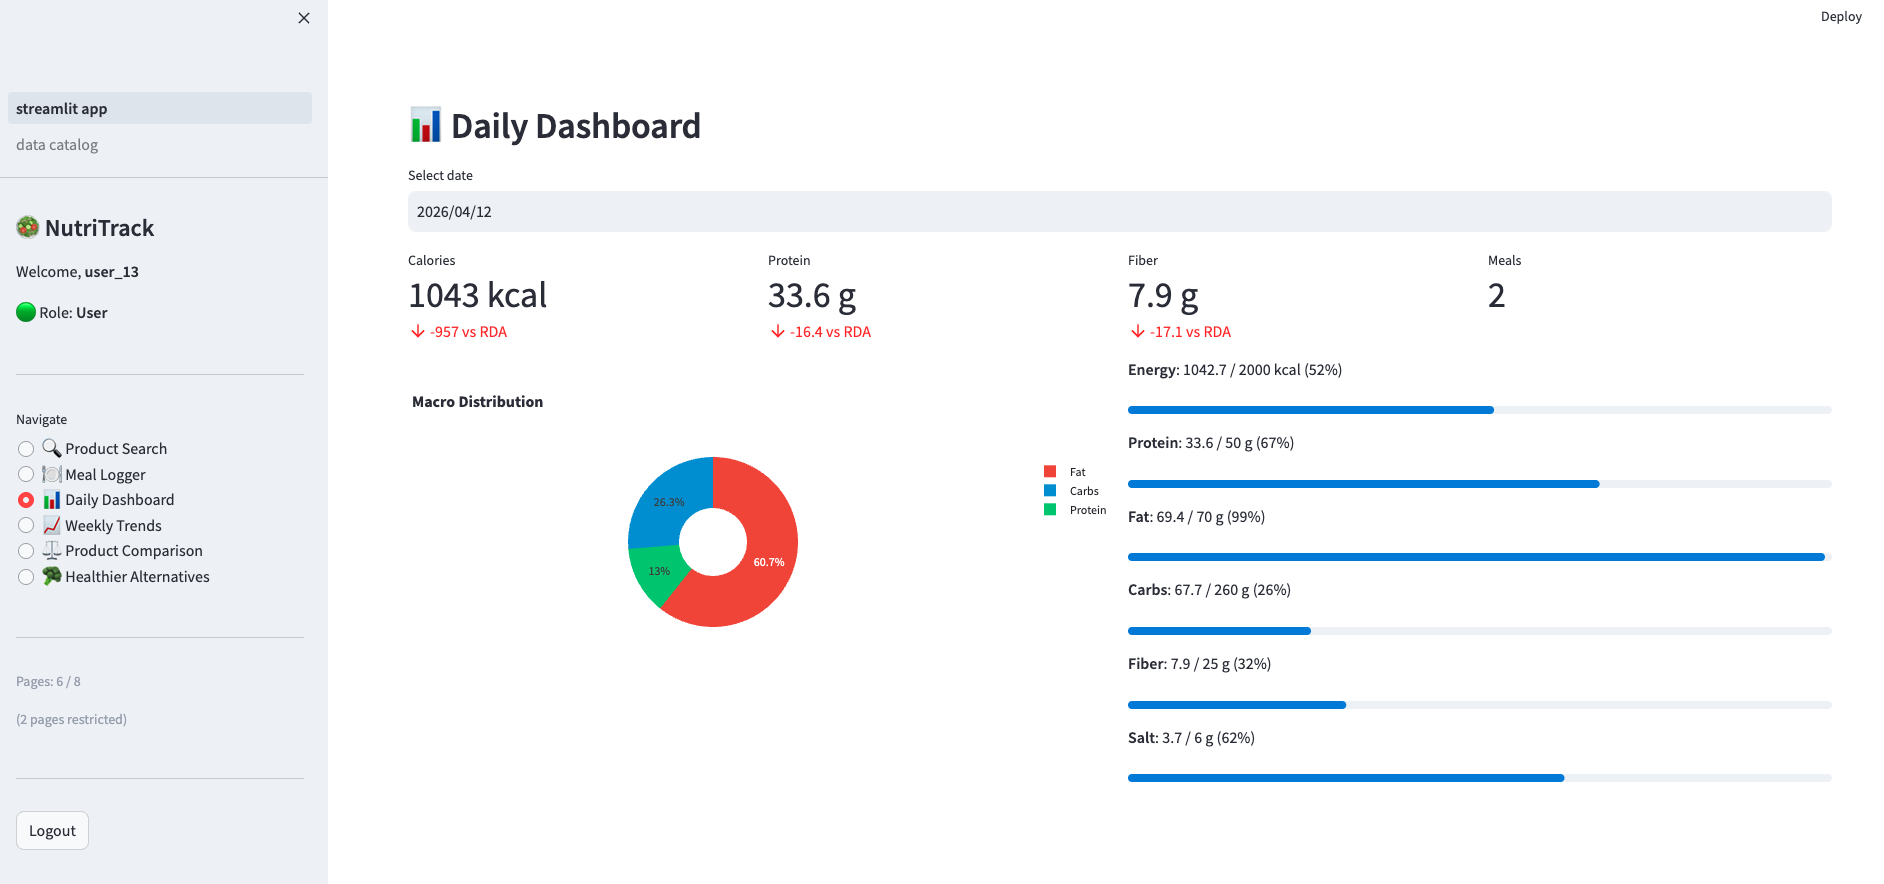
\includegraphics[width=\textwidth]{../../assets/screenshots/streamlit_user_dashboard.png}
\caption{Role utilisateur --- Tableau de bord quotidien montrant la distribution des macros (1\,043\,kcal,
33,6\,g de proteines), barres de progression AJR et nombre de repas. La barre laterale montre les 6 pages
disponibles pour le role \texttt{user}.}
\label{fig:streamlit-user}
\end{figure}

\begin{figure}[H]
\centering
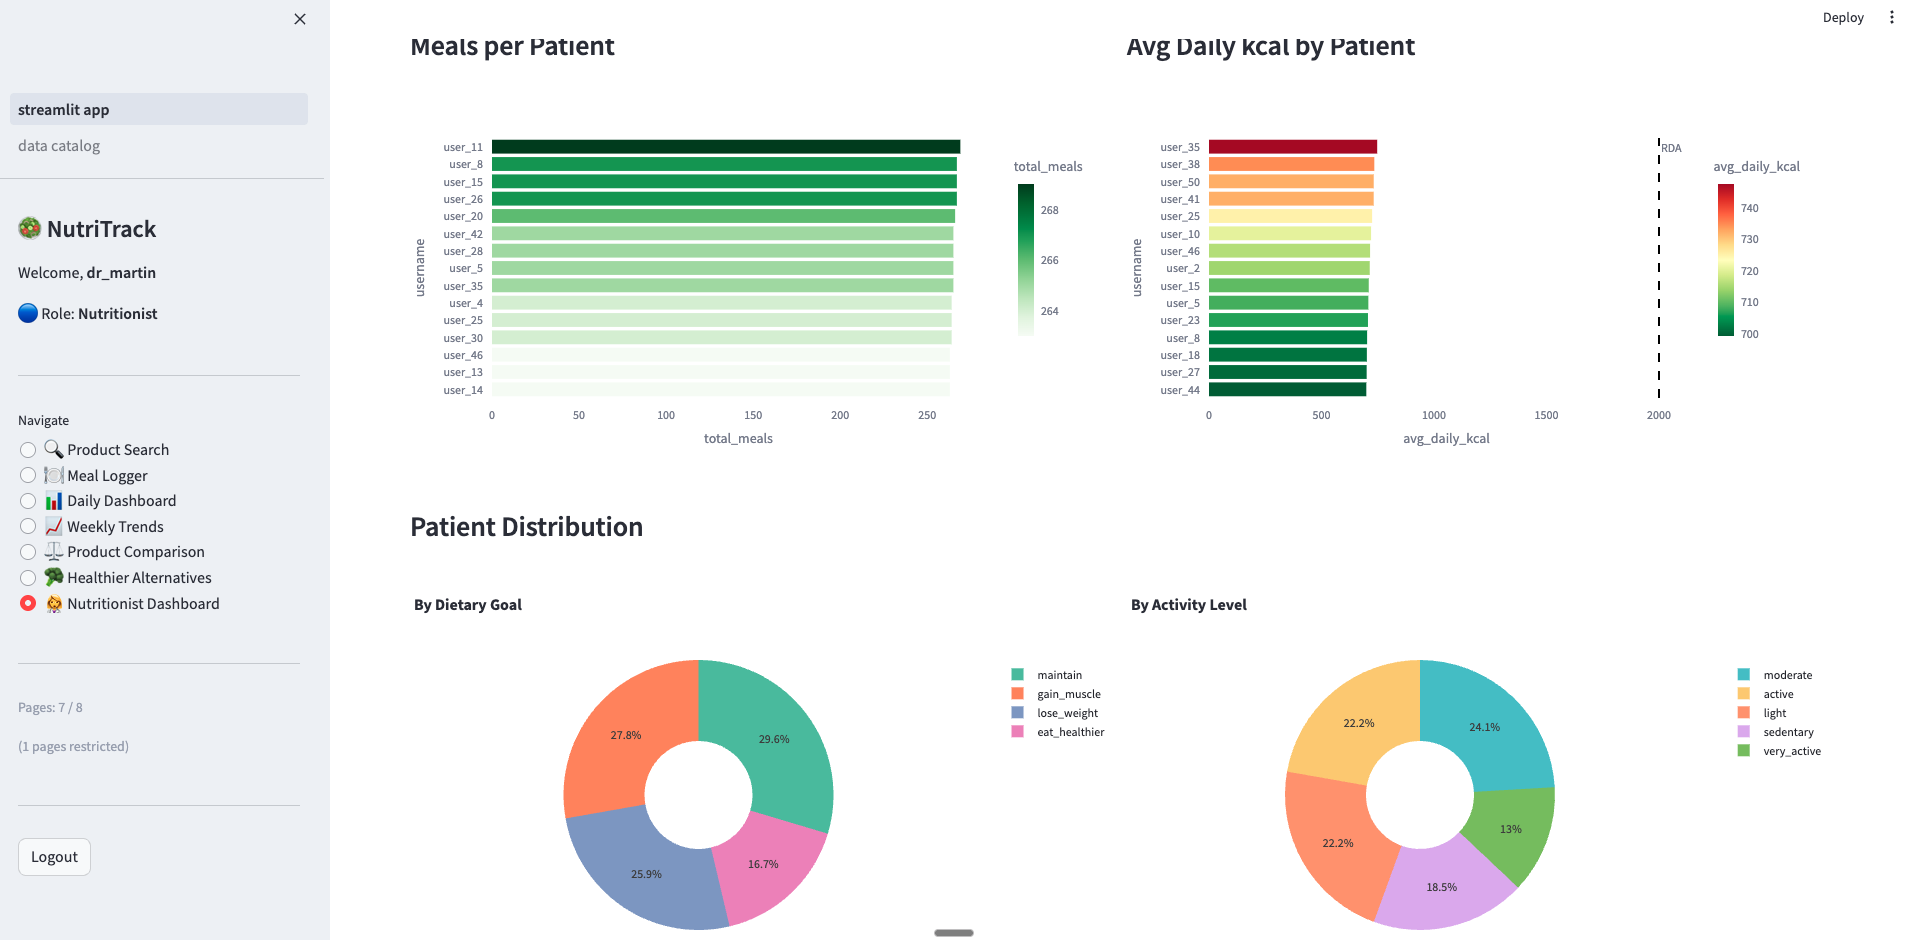
\includegraphics[width=\textwidth]{../../assets/screenshots/streamlit_nutritionist.png}
\caption{Role nutritionniste (dr\_martin) --- Vue d'ensemble patients avec repas par patient,
graphiques en barres de kcal quotidiennes moyennes, et distribution par objectif dietetique et
niveau d'activite. Cette page est masquee pour les roles \texttt{user} et \texttt{analyst}.}
\label{fig:streamlit-nutritionist}
\end{figure}

\begin{figure}[H]
\centering
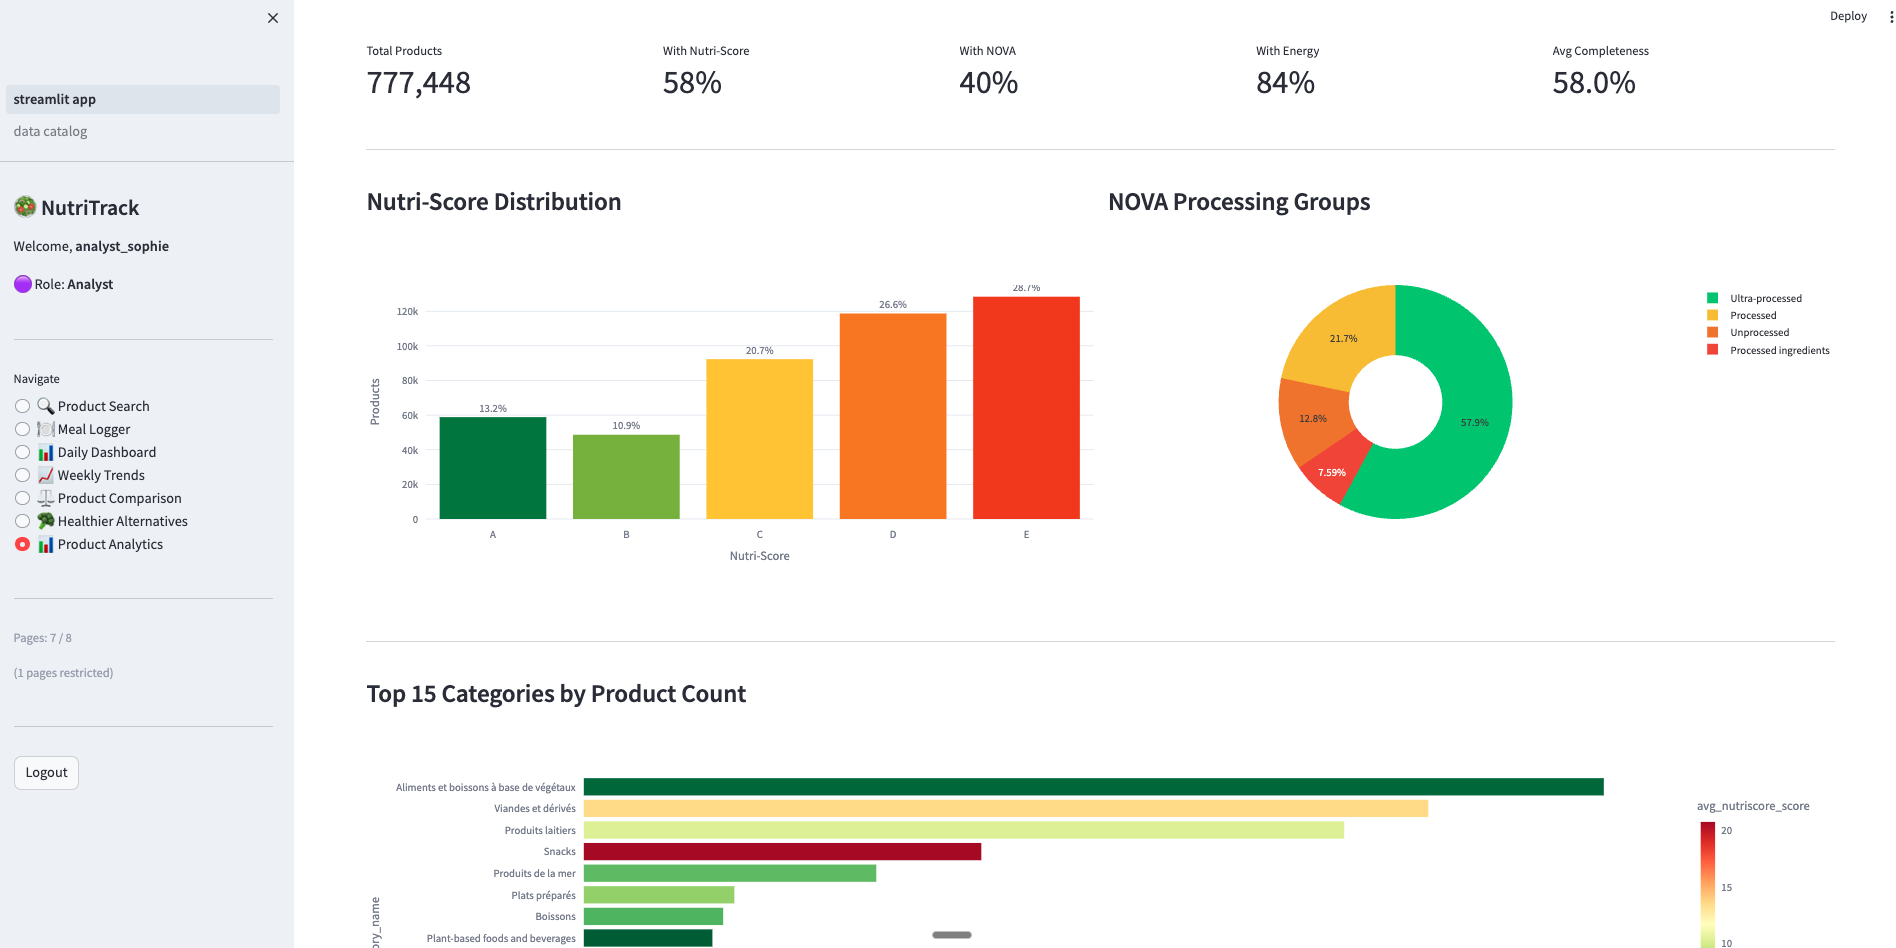
\includegraphics[width=\textwidth]{../../assets/screenshots/streamlit_analyst.png}
\caption{Role analyste (analyst\_sophie) --- Analytique produits montrant 777\,448 produits,
distribution Nutri-Score (A--E avec couleurs officielles), groupes de transformation NOVA, et
top 15 categories par nombre de produits. Cette page est masquee pour les roles \texttt{user} et
\texttt{nutritionist}.}
\label{fig:streamlit-analyst}
\end{figure}


% -----------------------------------------------------------
\section{Controles de qualite des donnees (\competence{C10})}
\label{sec:dq}

Six controles de qualite des donnees sont implementes dans le pipeline de
staging et enregistres dans la table \texttt{staging.data\_quality\_checks} :

\begin{table}[H]
\centering
\caption{Controles de qualite des donnees --- 6 validations automatisees}
\label{tab:dq-checks}
\begin{tabularx}{\textwidth}{C{0.5cm} L{3cm} L{4cm} L{5cm}}
\toprule
\textbf{\#} & \textbf{Controle} & \textbf{Regle} & \textbf{Action en cas d'echec} \\
\midrule
1 & Format code-barres & 8--14 chiffres, sans lettres & Enregistrement rejete \\
2 & Nom du produit present & \texttt{product\_name IS NOT NULL} et non vide & Enregistrement rejete \\
3 & Plage numerique & energie $\leq$ 1000, lipides $\leq$ 100, proteines $\leq$ 100, glucides $\leq$ 100 & Valeur mise a NULL \\
4 & Nutri-Score valide & Grade dans \{A, B, C, D, E\} & Valeur mise a NULL \\
5 & Groupe NOVA valide & Groupe dans \{1, 2, 3, 4\} & Valeur mise a NULL \\
6 & Detection de doublons & Code-barres unique (garder l'enregistrement le plus complet) & Doublon supprime \\
\bottomrule
\end{tabularx}
\end{table}


% -----------------------------------------------------------
\section{Analyse de conformite \rgpd{}}
\label{sec:rgpd-e4}

Le cadre complet de conformite \rgpd{} est documente en
Section~\ref{sec:e2} (Bloc~1, etude d'architecture \competence{C3}). Les
sept mesures --- registre des donnees personnelles, gestion du consentement,
minimisation des donnees, pseudonymisation, droit a la suppression,
retention automatisee et isolation du lac de donnees --- sont implementees
dans tous les composants decrits dans ce chapitre.


% =============================================================
% BLOC 3 : ENTREPOT DE DONNEES
% =============================================================
\chapter{Bloc 3 --- Elaborer et maintenir un entrepot de donnees}
\label{ch:bloc3}

% -----------------------------------------------------------
\section{Modelisation en schema en etoile (\competence{C13})}
\label{sec:c13}
{\small\evaluation{E5} | Schema en etoile : dimensions et faits}

\subsection{Approche : ascendante (Kimball)}

L'approche ascendante a ete choisie car : (1)~les questions analytiques
ont ete identifiees en amont, (2)~livraison de valeur plus rapide via
les datamarts, (3)~le schema operationnel est bien defini, et
(4)~extensibilite incrementale sans restructuration.

\subsection{Diagramme du schema en etoile}

\begin{figure}[H]
\centering
\resizebox{\textwidth}{!}{%
\begin{tikzpicture}[
  dim/.style={
    rectangle, rounded corners=3pt, draw=ntblue, fill=ntlightblue!20,
    minimum width=3cm, minimum height=2cm,
    font=\scriptsize, align=left, inner sep=5pt
  },
  fact/.style={
    rectangle, rounded corners=3pt, draw=ntgreen!80!black,
    fill=ntlightgreen!30, minimum width=3.5cm, minimum height=2.5cm,
    font=\scriptsize, align=left, inner sep=5pt
  },
  arr/.style={-{Stealth[length=5pt]}, thick, color=ntgray},
]

% Table de faits (centre)
\node[fact] (fact) {
  \textbf{fact\_daily\_nutrition}\\[2pt]
  daily\_nutrition\_id PK\\
  user\_key FK\\
  time\_key FK\\
  product\_key FK\\
  category\_key FK\\
  brand\_key FK\\[2pt]
  \textit{meal\_type}\\
  \textit{quantity\_g}\\
  \textit{energy\_kcal}\\
  \textit{fat\_g, proteins\_g}\\
  \textit{nutriscore\_score}
};

% Tables de dimensions
\node[dim, above left=1.5cm and 2.5cm of fact] (dimtime) {
  \textbf{dim\_time}\\[2pt]
  time\_key PK\\
  full\_date\\
  day\_of\_week\\
  month, quarter\\
  year, is\_weekend
};

\node[dim, above right=1.5cm and 2.5cm of fact] (dimuser) {
  \textbf{dim\_user} {\tiny\color{ntred}[SCD2]}\\[2pt]
  user\_key PK\\
  user\_hash (SHA256)\\
  age\_group\\
  dietary\_goal\\
  effective\_date\\
  is\_current
};

\node[dim, left=2.5cm of fact] (dimbrand) {
  \textbf{dim\_brand} {\tiny\color{ntorange}[SCD1]}\\[2pt]
  brand\_key PK\\
  brand\_name\\
  parent\_company\\
  last\_updated
};

\node[dim, right=2.5cm of fact] (dimcat) {
  \textbf{dim\_category}\\[2pt]
  category\_key PK\\
  category\_name\\
  parent\_category\\
  category\_level
};

\node[dim, below left=1.5cm and 2.5cm of fact] (dimproduct) {
  \textbf{dim\_product} {\tiny\color{ntred}[SCD2]}\\[2pt]
  product\_key PK\\
  barcode\\
  product\_name\\
  ingredients\_text\\
  effective\_date\\
  end\_date, is\_current
};

\node[dim, below right=1.5cm and 2.5cm of fact] (dimns) {
  \textbf{dim\_nutriscore}\\[2pt]
  nutriscore\_key PK\\
  grade (A--E)\\
  description\\
  color\_code\\
  score\_range
};

% Fleches
\draw[arr] (dimtime) -- (fact);
\draw[arr] (dimuser) -- (fact);
\draw[arr] (dimbrand) -- (fact);
\draw[arr] (dimcat) -- (fact);
\draw[arr] (dimproduct) -- (fact);
\draw[arr] (dimns) -- (fact);

\end{tikzpicture}%
}
\caption{Schema en etoile --- fact\_daily\_nutrition avec 6 dimensions}
\label{fig:star-schema}
\end{figure}

\subsection{Tables de dimensions et de faits}

\begin{table}[H]
\centering
\caption{Dimensions de l'entrepot de donnees}
\label{tab:dimensions}
\begin{tabularx}{\textwidth}{L{2.5cm} C{1.5cm} C{1.2cm} L{6.5cm}}
\toprule
\rowcolor{ntblue!80}
\textcolor{white}{\textbf{Dimension}} & \textcolor{white}{\textbf{SCD}} & \textcolor{white}{\textbf{Lignes}} & \textcolor{white}{\textbf{Description}} \\
\midrule
dim\_time & --- & 4\,018 & Dimension temporelle pre-remplie (2020--2030) \\
dim\_product & \cellcolor{ntlightblue!30}Type 2 & $\sim$777K & Attributs produit avec historique \\
dim\_brand & \cellcolor{ntlightgreen!40}Type 1 & $\sim$15K & Marques (ecrasement des corrections) \\
dim\_category & --- & $\sim$2K & Hierarchie de categories \\
dim\_country & \cellcolor{ntlightpurple!30}Type 3 & Ref. & Pays avec suivi d'expansion \\
dim\_user & \cellcolor{ntlightblue!30}Type 2 & $\sim$1K & Profils anonymises (SHA256) \\
dim\_nutriscore & --- & 5 & Reference Nutri-Score (A--E) \\
\bottomrule
\end{tabularx}
\end{table}

\begin{table}[H]
\centering
\caption{Tables de faits}
\label{tab:facts}
\begin{tabularx}{\textwidth}{L{3.5cm} L{4cm} L{5.5cm}}
\toprule
\textbf{Table de faits} & \textbf{Grain} & \textbf{Mesures} \\
\midrule
fact\_daily\_nutrition & 1 row / user + day + product & quantity, energy, fat, proteins, carbs, fiber, salt, nutriscore, nova \\
fact\_product\_market & 1 row / product + snapshot & nutriscore, nova, ecoscore, completeness, nutrition/100g \\
\bottomrule
\end{tabularx}
\end{table}


% -----------------------------------------------------------
\section{Implementation de l'entrepot de donnees (\competence{C14})}
\label{sec:c14}
{\small\evaluation{E5} | Creation et configuration de l'entrepot}

\textbf{Fichier :} \texttt{sql/init/02\_schema\_warehouse.sql} (360 lignes)

L'entrepot est implemente comme un schema separe (\texttt{dw}) au sein de
la meme instance PostgreSQL~16, cree automatiquement lors de
l'initialisation Docker Compose. Six vues analytiques (datamarts) sont
creees pour l'acces analyste: \texttt{dm\_user\_daily\_nutrition},
\texttt{dm\_product\_market\_by\_category},
\texttt{dm\_brand\_quality\_ranking},
\texttt{dm\_nutriscore\_distribution},
\texttt{dm\_nutrition\_trends},
\texttt{dm\_dw\_health}.

\textbf{Acces analyste via Streamlit :} Le role analyste se connecte a
l'entrepot via le tableau de bord Analytique produits
(Figure~\ref{fig:streamlit-analyst}), qui interroge les vues datamarts via
FastAPI en utilisant un role PostgreSQL en lecture seule
\texttt{analyst\_role} sur \texttt{dw.*}.

\subsection{Procedure de test}

\begin{table}[H]
\centering
\caption{Procedure de test de l'entrepot de donnees}
\label{tab:test-dw}
\begin{tabularx}{\textwidth}{L{3cm} L{2cm} L{7.5cm}}
\toprule
\textbf{Test} & \textbf{Portee} & \textbf{Verification} \\
\midrule
Creation du schema & Technique & Tables, index, vues crees sans erreurs \\
Alimentation dimensions & Fonctionnel & dim\_time = 4\,018 lignes ; dim\_nutriscore = 5 lignes (A--E) \\
SCD Type 2 & Fonctionnel & La mise a jour du produit cree une nouvelle ligne \texttt{is\_current=TRUE}, ferme l'ancienne \\
SCD Type 1 & Fonctionnel & La correction de marque ecrase sur place, met a jour \texttt{last\_updated} \\
Chargement des faits & Fonctionnel & FK valides vers les dimensions ; pas de cles orphelines \\
Vues datamarts & Fonctionnel & Les vues retournent des resultats ; \texttt{nutritionist\_role} peut faire SELECT \\
Controle d'acces & Securite & \texttt{app\_readonly} ne peut pas acceder au schema \texttt{dw} \\
\bottomrule
\end{tabularx}
\end{table}

\subsection{Retour d'experience sur la pile technique}

\begin{table}[H]
\centering
\caption{Retour d'experience sur la pile technique --- Entrepot de donnees}
\label{tab:tech-feedback}
\begin{tabularx}{\textwidth}{L{2.8cm} L{3cm} L{3.5cm} L{3.5cm}}
\toprule
\textbf{Technologie} & \textbf{Adequation projet} & \textbf{Avantages} & \textbf{Difficultes} \\
\midrule
PostgreSQL (OLTP+OLAP) & Bon a petite echelle & Instance unique, deploiement simple & Separation necessaire a plus grande echelle \\
Airflow pour ETL & Standard industriel & Interface web, tentatives, gestion des dependances & Configuration complexe (Celery, Redis, init) \\
PySpark ETL & Nettoyage distribue & Gere 800k+ lignes, pret pour cluster & Configuration plus lourde que du SQL pur \\
Isolation de schemas & Separation propre & Pas de contamination operationnel/analytique & Requetes inter-schemas dans l'ETL \\
\bottomrule
\end{tabularx}
\end{table}


% -----------------------------------------------------------
\section{Pipelines ETL (\competence{C15})}
\label{sec:c15}
{\small\evaluation{E5} | ETL pour les entrees/sorties de l'entrepot}

\textbf{Formats et volumes de donnees :}
\begin{itemize}[nosep]
  \item \textbf{Entree :} 798\,177 produits bruts depuis 3 sources (JSON API
        REST, Parquet OFF 4,2~Go, scraping ANSES/EFSA), totalisant $\sim$6~Go
        sur toutes les couches de stockage
  \item \textbf{Traitement :} PySpark 3.5 applique 7 regles de nettoyage,
        produisant 777\,116 enregistrements valides (97,4\,\% de retention)
  \item \textbf{Sortie :} Schema en etoile dans l'entrepot PostgreSQL
        (7 dimensions + 2 faits), analytique couche gold en Parquet MinIO
\end{itemize}

\textbf{Vue d'ensemble du pipeline :} 7 DAG Airflow avec 25 taches au total,
orchestres via des dependances ExternalTaskSensor pour la coordination
inter-DAG :

\begin{enumerate}[nosep]
  \item \texttt{etl\_extract\_off\_api} --- Extraction API REST quotidienne depuis Open Food Facts
  \item \texttt{etl\_extract\_parquet} --- Extraction Parquet + DuckDB hebdomadaire depuis l'export en masse OFF
  \item \texttt{etl\_extract\_scraping} --- Web scraping mensuel des donnees reglementaires ANSES/EFSA
  \item \texttt{etl\_aggregate\_clean} --- Nettoyage PySpark (agreger $\to$ nettoyer $\to$ valider $\to$ charger)
  \item \texttt{etl\_datalake\_ingest} --- Couches medallion bronze/silver/gold + agregats anonymises + catalogue
  \item \texttt{etl\_load\_warehouse} --- Alimentation des dimensions + faits du schema en etoile
  \item \texttt{etl\_backup\_maintenance} --- Sauvegardes hebdomadaires + nettoyage \rgpd{}
\end{enumerate}

\subsection{Flux de travail ETL}

\begin{figure}[H]
\centering
\resizebox{\textwidth}{!}{%
\begin{tikzpicture}[
  task/.style={
    rectangle, rounded corners=3pt, draw=ntorange, fill=ntorange!15,
    minimum width=3.2cm, minimum height=0.8cm,
    font=\scriptsize\bfseries, align=center
  },
  arr/.style={-{Stealth[length=5pt]}, thick, color=ntgray},
]

% Dimension tasks (parallel)
\node[task] (brands) {load\_dim\_brands\\{\tiny SCD Type 1}};
\node[task, right=0.4cm of brands] (cats) {load\_dim\_categories};
\node[task, right=0.4cm of cats] (prods) {load\_dim\_products\\{\tiny SCD Type 2}};
\node[task, right=0.4cm of prods] (users) {load\_dim\_users\\{\tiny SCD Type 2}};

% Fact tasks
\node[task, below=1.5cm of $(brands)!0.5!(cats)$, fill=ntlightgreen!40, draw=ntgreen] (factmarket) {load\_fact\_product\_market};
\node[task, below=1.5cm of $(prods)!0.5!(users)$, fill=ntlightgreen!40, draw=ntgreen] (factnutri) {load\_fact\_daily\_nutrition};

% Arrows
\draw[arr] (brands) -- (factmarket);
\draw[arr] (cats) -- (factmarket);
\draw[arr] (prods) -- (factmarket);
\draw[arr] (prods) -- (factnutri);
\draw[arr] (users) -- (factnutri);
\draw[arr] (cats) -- (factnutri);
\draw[arr] (brands) -- (factnutri);

% Labels
\node[font=\scriptsize\color{ntgray}, above=0.3cm of $(cats)!0.5!(prods)$]
  {Dimensions (parallele)};
\node[font=\scriptsize\color{ntgray}, below=0.3cm of $(factmarket)!0.5!(factnutri)$]
  {Faits (apres dimensions)};
\end{tikzpicture}%
}
\caption{Dependances des DAG ETL --- \texttt{etl\_load\_warehouse}}
\label{fig:etl-dag}
\end{figure}

\begin{figure}[H]
\centering
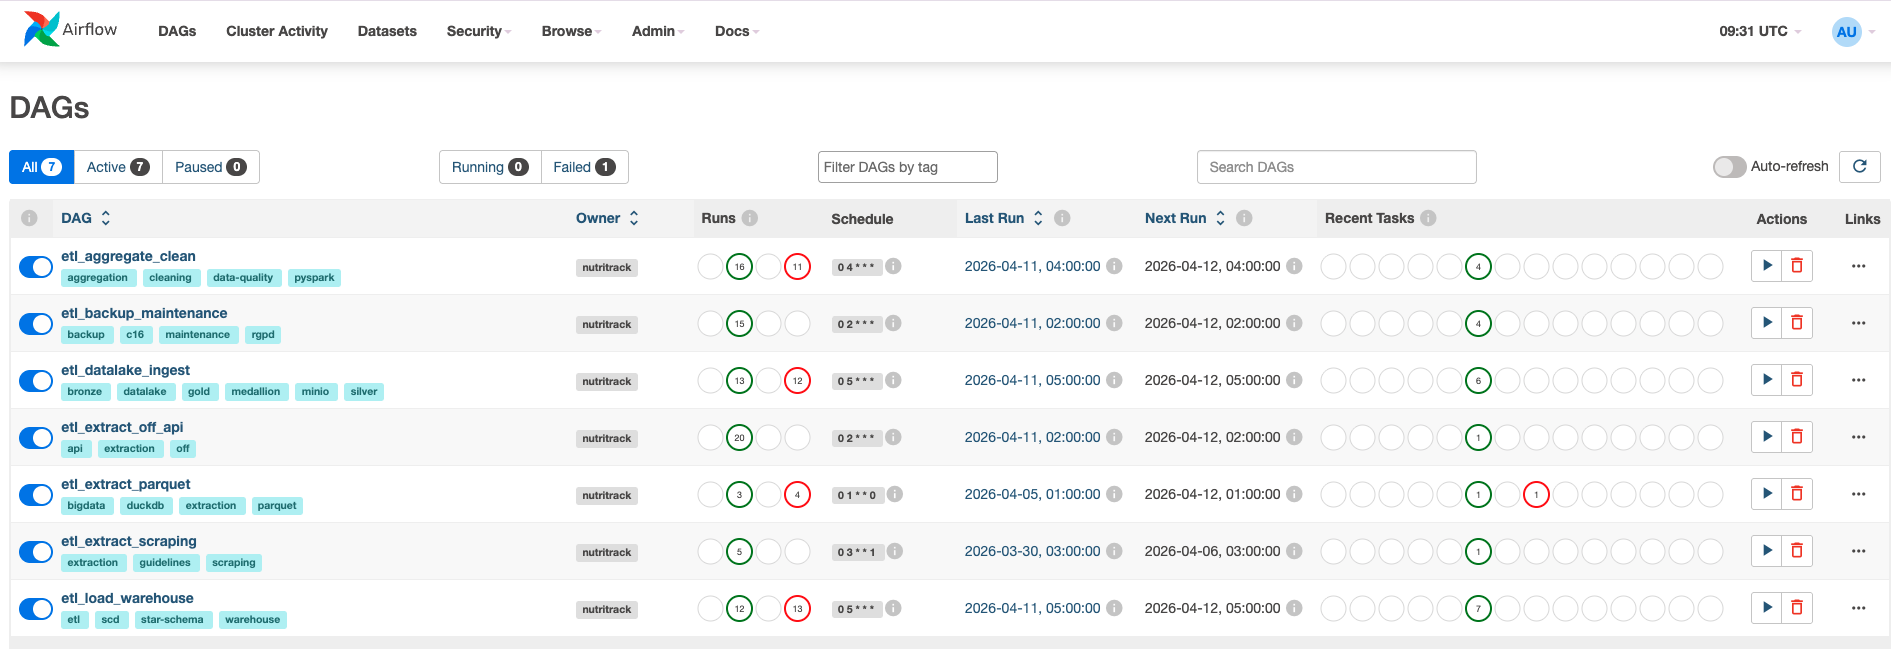
\includegraphics[width=\textwidth]{../../assets/screenshots/airflow_dags_list.png}
\caption{Interface Airflow --- Les 7 DAG avec historique d'execution et statut}
\label{fig:airflow-dags}
\end{figure}

\begin{figure}[H]
\centering
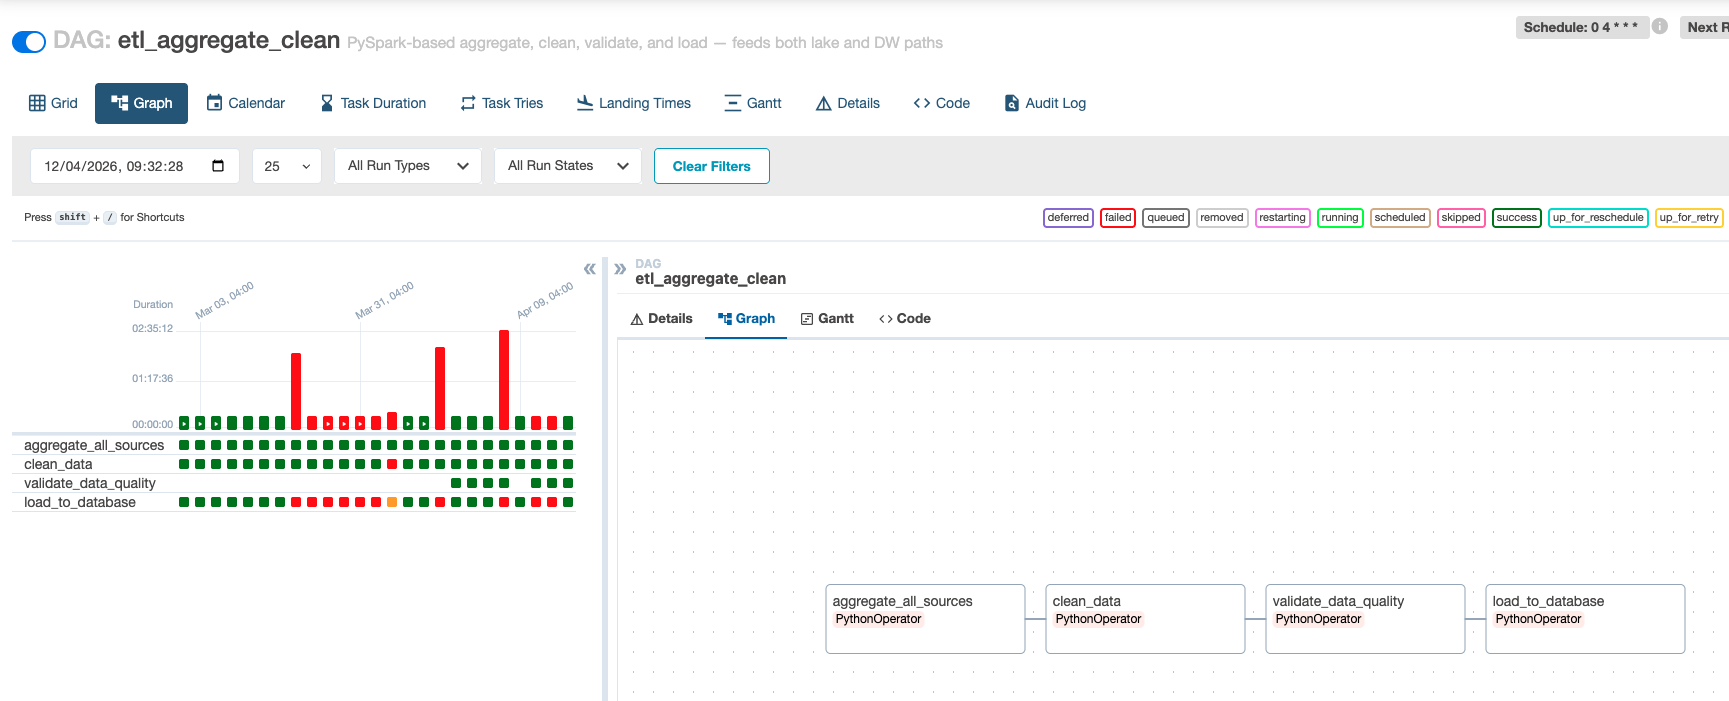
\includegraphics[width=\textwidth]{../../assets/screenshots/airflow_dag_graph.png}
\caption{Graphe du DAG \texttt{etl\_aggregate\_clean} --- Pipeline PySpark a 4 taches
(agreger $\to$ nettoyer $\to$ valider $\to$ charger)}
\label{fig:airflow-dag-graph}
\end{figure}


% -----------------------------------------------------------
\section{Maintenance et supervision de l'entrepot (\competence{C16})}
\label{sec:c16}
{\small\evaluation{E6} | Administration et supervision}

\subsection{Journalisation de l'activite}

La table \texttt{app.etl\_activity\_log} fournit une journalisation
structuree avec trois categories d'alertes :

\begin{table}[H]
\centering
\caption{Schema du journal d'activite ETL}
\label{tab:activity-log}
\begin{tabularx}{\textwidth}{L{3cm} L{2.5cm} L{7cm}}
\toprule
\textbf{Colonne} & \textbf{Type} & \textbf{Description} \\
\midrule
log\_id & SERIAL PK & Identifiant auto-incremente \\
log\_timestamp & TIMESTAMP & Horodatage de l'evenement \\
alert\_category & VARCHAR(20) & \texttt{CRITICAL}, \texttt{WARNING} ou \texttt{INFO} \\
dag\_id & VARCHAR(100) & Identifiant du DAG Airflow \\
task\_id & VARCHAR(100) & Identifiant de la tache Airflow \\
event\_type & VARCHAR(50) & \texttt{task\_failure}, \texttt{task\_success}, \texttt{sla\_miss}, etc. \\
message & TEXT & Description lisible de l'evenement \\
details & JSONB & Metadonnees structurees (duree, nombre d'enregistrements, erreurs) \\
acknowledged & BOOLEAN & Si l'incident a ete acquitte \\
\bottomrule
\end{tabularx}
\end{table}

\textbf{Donnees d'initialisation historiques :} La migration
\texttt{002\_seed\_etl\_activity\_log.sql} alimente environ 20 entrees
de journal couvrant 14 jours, incluant des executions ETL reussies, des
echecs transitoires avec reprise apres tentative, des completions de
sauvegarde, des depassements de SLA et des alertes de qualite des
donnees. Cela demontre une supervision continue tout au long du cycle de
vie du projet (\competence{C6}).

\subsection{Systeme d'alertes --- MailHog SMTP}

Les DAG Airflow sont configures avec des alertes email en cas d'echec,
delivrees via MailHog SMTP (un serveur de messagerie en mode
developpement) :

\begin{lstlisting}[language=Python, caption={Alerting default configuration (airflow/plugins/alerting.py)}]
ALERTING_DEFAULT_ARGS = {
    "email_on_failure": True,
    "email_on_retry": False,
    "email": ["admin@nutritrack.local"],
    "retries": 2,
    "retry_delay": timedelta(minutes=5),
}
\end{lstlisting}

\textbf{MailHog configuration} in \texttt{docker-compose.yml}:

\begin{lstlisting}[language=bash, caption={MailHog service and Airflow SMTP configuration}]
# MailHog service (port 8025 for web UI)
mailhog:
  image: mailhog/mailhog:latest
  ports:
    - "1025:1025"   # SMTP
    - "8025:8025"   # Web UI

# Airflow SMTP settings (environment variables)
AIRFLOW__SMTP__SMTP_HOST: mailhog
AIRFLOW__SMTP__SMTP_PORT: "1025"
AIRFLOW__SMTP__SMTP_STARTTLS: "false"
AIRFLOW__SMTP__SMTP_SSL: "false"
AIRFLOW__SMTP__SMTP_MAIL_FROM: airflow@nutritrack.local
\end{lstlisting}

Lorsqu'une tache echoue apres le nombre configure de tentatives, une
alerte email est envoyee a \texttt{admin@nutritrack.local} et peut etre
verifiee dans l'interface web MailHog sur le port~8025. Le plugin
d'alerte enregistre egalement chaque alerte, tentative et depassement
de SLA dans la table \texttt{app.etl\_activity\_log} pour un suivi
persistant.

\subsection{Indicateurs de niveau de service (SLA)}

\begin{table}[H]
\centering
\caption{Indicateurs de niveau de service}
\label{tab:sla}
\begin{tabularx}{\textwidth}{L{4cm} C{2cm} L{6.5cm}}
\toprule
\textbf{Indicateur} & \textbf{Cible} & \textbf{Mesure} \\
\midrule
Taux de reussite ETL & $>$~95\,\% & Historique d'execution des DAG Airflow \\
Fraicheur des donnees & $<$~24h & Horodatage de la derniere execution reussie \\
Temps de reponse requetes DW & $<$~5s & EXPLAIN ANALYZE sur les vues datamarts \\
Taux de reussite sauvegardes & 100\,\% & Entrees du journal de sauvegarde \\
Completude des donnees & $>$~80\,\% & Statistiques du rapport de nettoyage \\
\bottomrule
\end{tabularx}
\end{table}

\subsection{Priorisation des taches de maintenance (alignee ITIL)}

Les taches de maintenance suivent une matrice de priorite a quatre
niveaux inspiree de la gestion des incidents ITIL\,v4.

\begin{table}[H]
\centering
\caption{Matrice de priorite de maintenance (P1--P4)}
\label{tab:priority-matrix}
\begin{tabularx}{\textwidth}{C{1.2cm} C{1.5cm} C{1.8cm} C{2cm} L{5cm}}
\toprule
\textbf{Priorite} & \textbf{Severite} & \textbf{Reponse} & \textbf{Resolution} & \textbf{Exemples} \\
\midrule
P1 & Critique & $<$~1h & $<$~4h & Echec ETL bloquant l'analytique ; corruption BDD ; echec sauvegarde ; faille de securite \\
P2 & Eleve & $<$~4h & $<$~8h & Violation SLA (ETL $<$~95\,\%) ; fraicheur donnees $>$~24h ; echec DAG repete \\
P3 & Moyen & $<$~24h & $<$~3 jours & Echec DAG non critique ; requetes lentes ($>$~5s) ; erreurs tableau de bord \\
P4 & Faible & Sprint suivant & Prochaine version & Mises a jour doc ; changements cosmetiques ; demandes de nouveaux datamarts \\
\bottomrule
\end{tabularx}
\end{table}

\textbf{Regles d'attribution :}
\begin{itemize}[nosep]
  \item \textbf{P1 :} Attribue a l'ingenieur d'astreinte immediatement.
        Escalade vers le chef de projet apres 2\,h.
  \item \textbf{P2 :} Attribue pendant les heures ouvrees.
        Escalade apres 4\,h.
  \item \textbf{P3 :} Trie lors du standup quotidien, attribue au
        prochain ingenieur disponible.
  \item \textbf{P4 :} Ajoute au backlog de sprint, priorise lors de
        la planification de sprint.
\end{itemize}

\textbf{Chemin d'escalade :}
L1~(Ingenieur) $\to$ L2~(Ingenieur senior, si non resolu dans le delai
de reponse) $\to$ L3~(Chef de projet, P1$>$2h ou P2$>$4h).

\subsection{Tableau de bord de conformite SLA (Grafana)}

Un tableau de bord Grafana dedie (\texttt{monitoring/grafana/dashboards/sla-compliance.json})
offre une visibilite en temps reel sur tous les indicateurs de niveau de service :

\begin{table}[H]
\centering
\caption{Panneaux du tableau de bord SLA (10 panneaux)}
\label{tab:sla-dashboard}
\begin{tabularx}{\textwidth}{L{4cm} C{2cm} L{6.5cm}}
\toprule
\textbf{Panneau} & \textbf{Cible} & \textbf{Source Prometheus} \\
\midrule
Conformite SLA globale & $>$~95\,\% & Composite pondere de tous les indicateurs \\
Taux de reussite ETL & $>$~95\,\% & \texttt{airflow\_dagrun\_duration\_*} \\
Fraicheur des donnees & $<$~24h & \texttt{airflow\_dagrun\_start\_timestamp} \\
Completion des sauvegardes & 100\,\% & \texttt{airflow\_ti\_successes} (7j) \\
Temps de reponse requetes & $<$~5s & \texttt{pg\_stat\_activity\_max\_tx\_duration} \\
Utilisation du stockage & $<$~85\,\% & \texttt{pg\_database\_size\_bytes} \\
Taux de reussite ETL (7j) & $>$~95\,\% & Graphique de tendance 7 jours des executions DAG \\
Resultats des DAG (7j) & --- & Barres empilees : succes/echec/tentative \\
Nombre d'alertes actives & 0 & Comptage des entrees \texttt{CRITICAL} dans le journal d'activite \\
Score de qualite des donnees & $>$~90\,\% & Metriques de completude du rapport de nettoyage \\
\bottomrule
\end{tabularx}
\end{table}

Le tableau de bord permet l'identification proactive de la degradation
des performances avant que des violations de SLA ne surviennent, avec
des graphiques de tendance sur 7 jours pour le taux de reussite ETL et
les resultats des executions de DAG.

\begin{figure}[H]
\centering
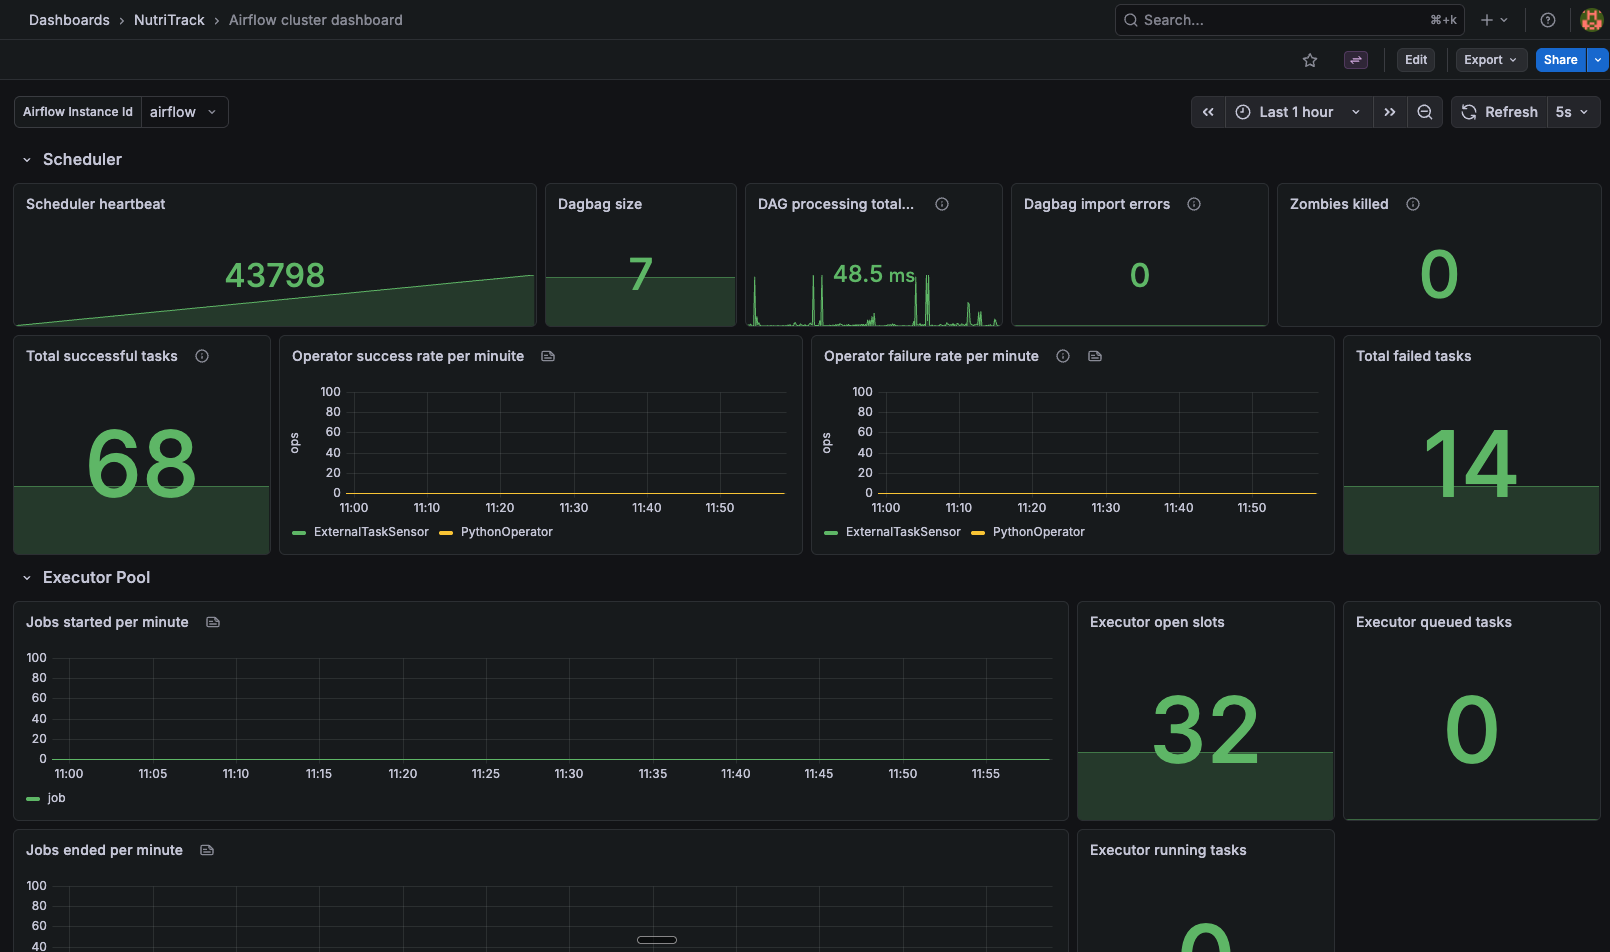
\includegraphics[width=\textwidth]{../../assets/screenshots/grafana_airflow.png}
\caption{Tableau de bord de supervision Grafana --- Battement du planificateur Airflow, temps de
traitement des DAG, taux de reussite des operateurs, statut du pool d'executeurs (43\,798 taches
reussies au total, 14 taches echouees au total)}
\label{fig:grafana-airflow}
\end{figure}

\subsection{Procedures de sauvegarde}

\textbf{Sauvegarde complete :} \texttt{make backup} (base de donnees complete)\\
\textbf{Sauvegarde partielle :} \texttt{make backup-dw} (schema DW uniquement)\\
Format : \texttt{pg\_dump --format=custom --compress=6}, telechargement
optionnel vers MinIO.

\textbf{Sauvegardes planifiees :} Le DAG \texttt{etl\_backup\_maintenance}
s'execute hebdomadairement et inclut des taches de sauvegarde du schema DW,
de verification de l'etat du stockage et de nettoyage des anciens fichiers
de sauvegarde.


\subsection{Procedure d'integration d'une nouvelle source}

Lorsqu'une nouvelle source de donnees doit etre integree a la plateforme,
la procedure en 6 etapes suivante est appliquee :

\begin{enumerate}[nosep]
  \item \textbf{Evaluation de la source :} Documenter la nouvelle source dans la
        topographie des donnees --- format (JSON, CSV, Parquet, API), volume,
        frequence de mise a jour, methode d'acces, licence et implications \rgpd{}.
  \item \textbf{Script d'extraction :} Creer un nouveau script d'extraction suivant
        la structure standard (point d'entree, init des dependances, config de
        connexion, logique metier, gestion d'erreurs, sauvegarde des resultats).
        Ajouter a Git avec documentation.
  \item \textbf{Ingestion bronze :} Configurer un nouveau DAG Airflow (ou ajouter
        des taches a un DAG existant) pour telecharger les donnees brutes vers
        le bucket bronze MinIO sous un nouveau prefixe
        (\texttt{new\_source/\{ds\}/*.format}).
  \item \textbf{Transformation silver :} Mettre a jour le pipeline de nettoyage
        PySpark pour inclure la nouvelle source. Ajouter des regles de nettoyage
        specifiques a la source si necessaire. Mettre a jour la configuration de
        correspondance de schema.
  \item \textbf{Integration DW :} Ajouter ou mettre a jour les taches de
        chargement des dimensions et tables de faits dans le DAG
        \texttt{etl\_load\_warehouse}. Si de nouvelles dimensions sont requises,
        creer des scripts de migration et mettre a jour le schema en etoile.
  \item \textbf{Validation et supervision :} Ajouter des controles de qualite des
        donnees pour la nouvelle source. Configurer les alertes pour les nouvelles
        taches DAG. Mettre a jour les metadonnees du catalogue de donnees dans
        MinIO. Executer un test de bout en bout.
\end{enumerate}

\subsection{Procedure de creation d'un nouvel acces}

Pour accorder l'acces a l'entrepot de donnees ou au lac de donnees a un
nouvel utilisateur ou groupe :

\begin{enumerate}[nosep]
  \item \textbf{Definir le perimetre d'acces :} Identifier quels schemas (app, dw),
        tables et buckets MinIO le nouvel utilisateur/groupe necessite. Appliquer
        le principe du moindre privilege. Documenter dans la matrice des droits
        d'acces (Tableau~\ref{tab:access-matrix}).
  \item \textbf{Configurer l'acces a la base de donnees :} Creer un role
        PostgreSQL avec les permissions appropriees :
        \begin{lstlisting}[language=SQL, numbers=none, frame=none, xleftmargin=0em, framexleftmargin=0em]
-- Example: new analyst role
CREATE ROLE new_analyst_role LOGIN PASSWORD 'secure_pwd';
GRANT USAGE ON SCHEMA dw TO new_analyst_role;
GRANT SELECT ON ALL TABLES IN SCHEMA dw TO new_analyst_role;
        \end{lstlisting}
  \item \textbf{Configurer l'acces au lac de donnees :} Creer une politique
        MinIO limitee aux buckets requis et l'appliquer a l'utilisateur/groupe :
        \begin{lstlisting}[language=bash, numbers=none, frame=none, xleftmargin=0em, framexleftmargin=0em]
# Example: read-only access to gold bucket
mc admin policy create myminio gold-readonly gold-policy.json
mc admin user add myminio new_analyst secure_pwd
mc admin policy attach myminio gold-readonly --user new_analyst
        \end{lstlisting}
\end{enumerate}

\subsection{Documentation de scalabilite}

\begin{table}[H]
\centering
\caption{Procedures de scalabilite pour l'evolution de la plateforme}
\label{tab:scalability}
\begin{tabularx}{\textwidth}{L{3cm} L{3cm} L{6.5cm}}
\toprule
\textbf{Dimension} & \textbf{Etat actuel} & \textbf{Procedure de mise a l'echelle} \\
\midrule
Espace de stockage & PostgreSQL : $\sim$2~Go ; MinIO : $\sim$4~Go & PostgreSQL : ajouter des tablespaces sur de nouveaux volumes. MinIO : ajouter des noeuds de stockage au cluster (le codage par effacement supporte 4--16 noeuds). Redimensionnement du volume Docker via le systeme de fichiers hote. \\
Nouveaux datamarts & 6 vues analytiques & Creer une nouvelle vue SQL dans le schema \texttt{dw} ; accorder SELECT au role cible ; ajouter l'endpoint FastAPI et la page Streamlit correspondants ; documenter dans le catalogue de donnees. \\
Capacite de calcul & Hote Docker unique & Migrer vers Docker Swarm ou Kubernetes pour la scalabilite horizontale. Airflow : basculer de CeleryExecutor vers KubernetesExecutor. PySpark : se connecter a un cluster standalone ou YARN. \\
Nouvelles sources & 3 sources & Suivre la procedure d'integration d'une nouvelle source en 6 etapes ci-dessus. \\
Utilisateurs supplementaires & 4 groupes de roles & Suivre la procedure de creation d'un nouvel acces en 3 etapes ci-dessus. \\
\bottomrule
\end{tabularx}
\end{table}

\subsection{Registre \rgpd{} et procedures de tri (C16)}

Le registre des donnees personnelles (Tableau~\ref{tab:rgpd}) est maintenu
et mis a jour chaque fois que de nouvelles categories de donnees sont
introduites. Les procedures de tri et de suppression sont automatisees :

\begin{itemize}[nosep]
  \item \textbf{Tri automatise :} La fonction \texttt{rgpd\_cleanup\_expired\_data()}
        s'execute mensuellement (planifiee via Airflow) et effectue :
        (1)~la suppression des enregistrements de repas de plus de 2 ans,
        (2)~la desactivation des comptes utilisateurs au-dela de la retention
        de 3 ans, (3)~la journalisation de toutes les suppressions dans le
        journal d'activite.
  \item \textbf{Droit a la suppression manuel :} Sur demande de l'utilisateur,
        un administrateur peut executer
        \texttt{DELETE FROM app.users WHERE user\_id = \$UUID} qui se propage
        en cascade a tous les repas et elements de repas associes.
  \item \textbf{Conformite du lac de donnees :} Aucune donnee personnelle n'est
        stockee dans le lac de donnees. Les regles de cycle de vie MinIO
        imposent la suppression automatique des donnees bronze a 90 jours et
        des sauvegardes a 30 jours.
\end{itemize}


% -----------------------------------------------------------
\section{Variations de dimensions SCD (\competence{C17})}
\label{sec:c17}
{\small\evaluation{E6} | Kimball Type 1, 2, 3}

\begin{figure}[H]
\centering
\resizebox{\textwidth}{!}{%
\begin{tikzpicture}[
  scd/.style={
    rectangle, rounded corners=5pt, draw=#1, fill=#1!10,
    minimum width=4.5cm, minimum height=2.5cm,
    font=\scriptsize, align=left, inner sep=8pt
  },
  title/.style={font=\small\bfseries\color{#1}},
]

% SCD Type 1
\node[scd=ntorange] (scd1) at (0,0) {
  \textbf{\color{ntorange}SCD Type 1 : Ecrasement}\\[3pt]
  \textbf{Cas d'usage :} Correction de nom de marque\\
  \textbf{Table :} dim\_brand\\
  \textbf{Action :} UPDATE direct\\
  \textbf{Historique :} Non conserve\\[2pt]
  {\tiny \texttt{SET brand\_name = p\_new}}\\
  {\tiny \texttt{SET last\_updated = NOW()}}
};

% SCD Type 2
\node[scd=ntred, right=0.8cm of scd1] (scd2) {
  \textbf{\color{ntred}SCD Type 2 : Historique}\\[3pt]
  \textbf{Cas d'usage :} Reformulation de produit\\
  \textbf{Table :} dim\_product, dim\_user\\
  \textbf{Action :} Fermer ancien + inserer nouveau\\
  \textbf{Historique :} Complet\\[2pt]
  {\tiny \texttt{end\_date, is\_current}}\\
  {\tiny \texttt{effective\_date}}
};

% SCD Type 3
\node[scd=ntblue, right=0.8cm of scd2] (scd3) {
  \textbf{\color{ntblue}SCD Type 3 : Colonne}\\[3pt]
  \textbf{Cas d'usage :} Expansion geographique\\
  \textbf{Table :} dim\_country\\
  \textbf{Action :} Stocker la valeur precedente\\
  \textbf{Historique :} 1 version anterieure\\[2pt]
  {\tiny \texttt{previous\_country\_list}}\\
  {\tiny \texttt{= old country\_name}}
};

\end{tikzpicture}%
}
\caption{Trois types de dimensions a evolution lente implementes}
\label{fig:scd-types}
\end{figure}


% =============================================================
% BLOC 4 : LAC DE DONNEES
% =============================================================
\chapter{Bloc 4 --- Lac de donnees}
\label{ch:bloc4}

% -----------------------------------------------------------
\section{Architecture du lac de donnees (\competence{C18})}
\label{sec:c18}
{\small\evaluation{E7} | Conception de l'architecture}

\subsection{Architecture medallion}

\begin{figure}[H]
\centering
\resizebox{\textwidth}{!}{%
\begin{tikzpicture}[
  layer/.style={
    rectangle, rounded corners=8pt, draw=#1!80!black, fill=#1!20,
    minimum width=4cm, minimum height=3.5cm,
    font=\small, align=center, inner sep=10pt
  },
  arr/.style={-{Stealth[length=6pt]}, very thick, color=ntgray},
  content/.style={font=\tiny, align=left, text=ntgray},
]

% Bronze
\node[layer=bronze] (br) {};
\node[font=\bfseries\color{bronze!80!black}, anchor=north] at (br.north)
  {BRONZE};
\node[content, anchor=center] at (br.center) {
  api/\{ds\}/*.json\\
  parquet/\{ds\}/*.parquet\\
  scraping/\{ds\}/*.json\\
  duckdb/\{ds\}/*.parquet\\[3pt]
  \_manifests/\{ds\}.json\\[3pt]
  \textit{Raw data}\\
  \textit{Retention: 90 days}
};

% Silver
\node[layer=silver, right=1.5cm of br] (sv) {};
\node[font=\bfseries\color{ntgray}, anchor=north] at (sv.north) {SILVER};
\node[content, anchor=center] at (sv.center) {
  products/\{ds\}/\\
  \quad products\_cleaned.parquet\\[3pt]
  \_reports/\\
  \quad cleaning\_report.json\\[5pt]
  \textit{Cleaned data}\\
  \textit{Retention: 1 year}
};

% Gold
\node[layer=gold, right=1.5cm of sv] (gd) {};
\node[font=\bfseries\color{gold!80!black}, anchor=north] at (gd.north)
  {GOLD};
\node[content, anchor=center] at (gd.center) {
  analytics/\{ds\}/\\
  \quad nutrition\_patterns.parquet\\
  \quad popular\_products.parquet\\
  \quad brand\_rankings.parquet\\
  \quad category\_stats.parquet\\[3pt]
  \textit{Anonymized aggregates}\\
  \textit{Retention: indefinite}
};

% Arrows
\draw[arr] (br) -- (sv);
\draw[arr] (sv) -- (gd);

% Labels
\node[font=\tiny\color{ntgray}, above=0.1cm of $(br)!0.5!(sv)$] {Nettoyage};
\node[font=\tiny\color{ntgray}, above=0.1cm of $(sv)!0.5!(gd)$] {Agregation};

% MinIO label
\node[font=\footnotesize\bfseries\color{ntgray},
      above=0.8cm of sv] {MinIO (S3-compatible) --- Medallion Architecture};

\end{tikzpicture}%
}
\caption{Architecture medallion du lac de donnees (Bronze / Silver / Gold)}
\label{fig:medallion}
\end{figure}

\subsection{Repondre aux 3~V}

\begin{table}[H]
\centering
\caption{Contraintes et solutions Volume, Velocite, Variete}
\label{tab:3v}
\begin{tabularx}{\textwidth}{C{1.5cm} L{4cm} L{7.5cm}}
\toprule
\textbf{V} & \textbf{Defi} & \textbf{Solution} \\
\midrule
Volume & 3M+ produits ($\sim$5\,Go Parquet) & DuckDB lit le Parquet sans chargement en memoire ; MinIO monte jusqu'au petaoctet \\
Variete & JSON, Parquet, CSV, SQL & Bronze stocke les formats bruts ; Silver normalise en Parquet unifie \\
Velocite & Mises a jour API quotidiennes, masse hebdomadaire & DAG Airflow sur calendrier ; Bronze preserve les instantanes par \{ds\}/ \\
\bottomrule
\end{tabularx}
\end{table}

\subsection{Comparaison des outils de catalogue}

\begin{table}[H]
\centering
\caption{Comparaison et selection des outils de catalogue}
\label{tab:catalog-compare}
\begin{tabularx}{\textwidth}{L{2.5cm} C{2.5cm} C{2.5cm} C{3.5cm}}
\toprule
\textbf{Critere} & \textbf{Apache Atlas} & \textbf{DataHub} & \textbf{Catalogue JSON} \\
\midrule
Complexite & Elevee & Moyenne & \textbf{Faible} \\
Temps de mise en place & Jours & Heures & \textbf{Minutes} \\
Integration & Hadoop & API REST & \textbf{MinIO natif} \\
Cout en ressources & Eleve (JVM) & Moyen & \textbf{Minimal} \\
\bottomrule
\end{tabularx}
\end{table}

\textbf{Selection :} Catalogue JSON personnalise --- choisi pour sa
surcharge minimale, son integration directe avec MinIO et sa suffisance
a l'echelle du projet.


% -----------------------------------------------------------
\section{Composants d'infrastructure (\competence{C19})}
\label{sec:c19}
{\small\evaluation{E7} | Installation et configuration}

L'ensemble de l'infrastructure est deployable dans un environnement de
developpement via Docker Compose. L'installation a ete testee sur macOS
(Apple Silicon) et Linux (Ubuntu 22.04) sans erreurs.

\textbf{Prerequisites :} Docker Engine 24+, Docker Compose v2, 8~Go de RAM
minimum, 10~Go d'espace disque libre.

\begin{lstlisting}[language=bash, caption={Deploiement de l'infrastructure}]
# Cloner le depot
git clone https://github.com/Reetika12795/NutriTrack.git
cd NutriTrack/nutritrack

# Demarrer les 15 services
docker compose up -d

# Attendre ~60 secondes, puis verifier
docker compose ps
# Resultat attendu : 15 services en cours d'execution
\end{lstlisting}

\textbf{Inventaire des services (15 services) :}

\begin{table}[H]
\centering
\caption{Inventaire des services Docker Compose}
\label{tab:services}
\begin{tabularx}{\textwidth}{C{0.5cm} L{3cm} L{2.5cm} C{1.5cm} L{4.5cm}}
\toprule
\textbf{\#} & \textbf{Service} & \textbf{Image} & \textbf{Port} & \textbf{Fonction} \\
\midrule
1 & PostgreSQL & postgres:16-alpine & 5432 & Base de donnees OLTP + OLAP \\
2 & Redis & redis:7-alpine & 6379 & Cache + broker Celery \\
3 & MinIO & minio/minio:latest & 9000/9001 & Stockage objet compatible S3 \\
4 & Airflow Webserver & custom (Python 3.11) & 8080 & Interface web ETL \\
5 & Airflow Scheduler & custom (Python 3.11) & --- & Planification des DAG \\
6 & Airflow Worker & custom (Python 3.11) & --- & Execution des taches (Celery) \\
7 & Airflow Init & custom (Python 3.11) & --- & Migration BDD + creation utilisateur \\
8 & FastAPI & custom (Python 3.11) & 8000 & API REST \\
9 & Streamlit & custom (Python 3.11) & 8501 & Interface utilisateur \\
10 & Prometheus & prom/prometheus & 9090 & Collecte de metriques \\
11 & Grafana & grafana/grafana & 3000 & Tableaux de bord + alertes \\
12 & MailHog & mailhog/mailhog & 8025 & Serveur email de dev \\
13 & postgres-exporter & prometheuscommunity & 9187 & Metriques PostgreSQL \\
14 & MinIO createbuckets & minio/mc & --- & Initialisation des buckets \\
15 & DuckDB sidecar & duckdb/duckdb & --- & Analytique Parquet ad-hoc \\
\bottomrule
\end{tabularx}
\end{table}

\textbf{Configuration du systeme de stockage :}
\begin{itemize}[nosep]
  \item \textbf{PostgreSQL :} 4 schemas (\texttt{app}, \texttt{raw}, \texttt{staging},
        \texttt{dw}), initialises via les scripts de migration SQL dans \texttt{sql/init/}
  \item \textbf{MinIO :} 4 buckets (\texttt{bronze}, \texttt{silver}, \texttt{gold},
        \texttt{backups}), crees automatiquement par le conteneur d'initialisation
        \texttt{createbuckets} avec les regles de cycle de vie appliquees
  \item \textbf{Redis :} Cache en memoire pour le broker Celery Airflow et la
        gestion des sessions API
\end{itemize}

\textbf{Outils batch et temps reel :}
\begin{itemize}[nosep]
  \item \textbf{Batch :} Les DAG Airflow (7 DAG, 25 taches) orchestrent tous
        les flux ETL sur des calendriers configurables (quotidien, hebdomadaire)
  \item \textbf{Temps reel :} FastAPI fournit un acces synchrone aux requetes
        de la base de donnees ; Streamlit fournit des mises a jour de tableau
        de bord en temps reel
  \item \textbf{Catalogue :} Le catalogue JSON dans MinIO est connecte au
        systeme de stockage et mis a jour automatiquement par les pipelines ETL
\end{itemize}


% -----------------------------------------------------------
\section{Gestion du catalogue de donnees (\competence{C20})}
\label{sec:c20}
{\small\evaluation{E7} | Catalogue, cycle de vie et supervision}

Le catalogue de donnees est stocke sous forme de
\texttt{\_catalog/metadata.json} dans chaque bucket MinIO, mis a jour
quotidiennement par le pipeline ETL. Il documente pour chaque jeu de
donnees : description, format, frequence de mise a jour, source, schema,
proprietaire, qualite et lignee.

\subsection{Methode d'alimentation par source}

\begin{table}[H]
\centering
\caption{Selection de la methode d'alimentation par source de donnees}
\label{tab:feed-methods}
\begin{tabularx}{\textwidth}{L{2.5cm} L{2cm} L{3cm} L{5cm}}
\toprule
\textbf{Source} & \textbf{Methode} & \textbf{Frequence} & \textbf{Justification} \\
\midrule
API REST OFF & Batch (extraction API) & Quotidien & Limite aux requetes par categorie ; debit limite ; adapte aux mises a jour incrementales \\
Parquet OFF & Batch (telechargement fichier) & Hebdomadaire & Rafraichissement complet du jeu de donnees ; fichier de 4,2~Go trop volumineux pour des telechargements frequents \\
ANSES/EFSA & Batch (scraping) & Mensuel & Les valeurs de reference changent rarement ; exploration respectueuse \\
PostgreSQL (app) & Batch (extraction SQL) & Quotidien & Extraire les enregistrements nouveaux/modifies depuis la derniere execution via l'horodatage \texttt{updated\_at} \\
Analytique DuckDB & A la demande & Selon besoin & Requetes analytiques declenchees par demande utilisateur ou rapport planifie \\
\bottomrule
\end{tabularx}
\end{table}

\subsection{Mises a jour des metadonnees du catalogue}

Les metadonnees du catalogue de donnees sont mises a jour a chaque execution
ETL via le processus suivant :
\begin{enumerate}[nosep]
  \item Chaque tache DAG ecrit un fichier manifeste (\texttt{\_manifests/\{ds\}.json})
        contenant : source, nombre d'enregistrements, tailles de fichiers, hash du
        schema et horodatage.
  \item La tache de mise a jour du catalogue agrege les manifestes et met a jour
        \texttt{\_catalog/metadata.json} avec : date de derniere mise a jour, nombre
        total d'enregistrements, version du schema, lignee des donnees
        (source $\to$ bronze $\to$ silver $\to$ gold) et metriques de qualite issues
        du rapport de nettoyage.
  \item Le navigateur de catalogue de donnees Streamlit fournit une interface en
        lecture seule pour explorer les metadonnees du catalogue, les schemas des
        jeux de donnees et la lignee.
\end{enumerate}

\subsection{Procedures de suppression et mise a jour basees sur le cycle de vie}

\begin{table}[H]
\centering
\caption{Regles de cycle de vie des donnees par bucket}
\label{tab:lifecycle}
\begin{tabularx}{\textwidth}{L{2cm} L{2cm} L{3cm} L{5.5cm}}
\toprule
\textbf{Bucket} & \textbf{Retention} & \textbf{Methode de suppression} & \textbf{Procedure} \\
\midrule
Bronze & 90 jours & Regle de cycle de vie MinIO & Expiration automatique ; anciens instantanes supprimes apres 90 jours pour liberer du stockage \\
Silver & 1 an & Manuel / cycle de vie & Jeux de donnees nettoyes obsoletes remplaces par de nouvelles executions ; anciennes versions expirent apres 1 an \\
Gold & Indefinie & Manuel uniquement & Analytique agregee conservee indefiniment ; suppression necessite approbation admin \\
Sauvegardes & 30 jours & Regle de cycle de vie MinIO & Anciennes sauvegardes automatiquement purgees ; les 4 sauvegardes hebdomadaires les plus recentes toujours conservees \\
\bottomrule
\end{tabularx}
\end{table}

\textbf{Procedures de mise a jour :}
\begin{itemize}[nosep]
  \item \textbf{Rafraichissement des donnees :} Les nouvelles executions ETL ecrivent
        dans des chemins partitionnes par date (\texttt{\{ds\}/}), preservant les
        versions precedentes jusqu'a l'expiration du cycle de vie.
  \item \textbf{Evolution du schema :} Si le schema source change, le pipeline de
        nettoyage est mis a jour, une nouvelle version du schema est enregistree dans
        le catalogue, et les anciennes donnees silver sont marquees comme obsoletes.
  \item \textbf{Suppression reglementaire :} Pour la conformite \rgpd{}, toute donnee
        personnelle ingeree par inadvertance dans bronze est immediatement supprimee
        et journalisee comme un evenement CRITICAL dans le journal d'activite.
\end{itemize}

\subsection{Supervision avec alertes}

Le lac de donnees est supervise via les metriques Prometheus et les tableaux
de bord Grafana avec des alertes automatisees :

\begin{table}[H]
\centering
\caption{Supervision du lac de donnees --- alertes et seuils}
\label{tab:lake-monitoring}
\begin{tabularx}{\textwidth}{L{3.5cm} C{2cm} L{3cm} L{4cm}}
\toprule
\textbf{Metrique} & \textbf{Seuil} & \textbf{Canal d'alerte} & \textbf{Action} \\
\midrule
Utilisation disque MinIO & $>$~85\,\% & Grafana $\to$ MailHog & Declencher le nettoyage du cycle de vie ; etendre le stockage \\
Statut serveur MinIO & DOWN & Grafana $\to$ MailHog & Redemarrer le conteneur ; escalader si persistant \\
Echec d'alimentation ETL & 2 consecutifs & Airflow $\to$ MailHog & Reessayer ; verifier la disponibilite de la source ; journaliser CRITICAL \\
Age de mise a jour du catalogue & $>$~48h & Grafana $\to$ MailHog & Investiguer le pipeline ETL ; verifier le planificateur des DAG \\
Volume de donnees bronze & $>$~10~Go & Panneau Grafana & Revoir les regles de cycle de vie ; archiver les anciens instantanes \\
Utilisation memoire & $>$~90\,\% & Grafana $\to$ MailHog & Augmenter la capacite de calcul ; optimiser les parametres memoire PySpark \\
\bottomrule
\end{tabularx}
\end{table}

Grafana alert rules are defined in \texttt{monitoring/grafana/provisioning/alerting/}
and configured to send notifications via MailHog SMTP for development
and via email/Slack for production deployment.


% -----------------------------------------------------------
\section{Gouvernance des donnees (\competence{C21})}
\label{sec:c21}
{\small\evaluation{E7} | Regles de gouvernance et controle d'acces}

\begin{table}[H]
\centering
\caption{Matrice des droits d'acces par groupe}
\label{tab:access-matrix}
\arrayrulecolor{ntblue}
\rowcolors{2}{ntlightblue!15}{white}
\begin{tabularx}{\textwidth}{L{2.3cm} L{2.3cm} L{3.2cm} C{1.5cm} L{3.2cm}}
\toprule
\rowcolor{ntblue}
\textcolor{white}{\textbf{Group}} & \textcolor{white}{\textbf{PG Role}} & \textcolor{white}{\textbf{MinIO Policy}} & \textcolor{white}{\textbf{API Role}} & \textcolor{white}{\textbf{Streamlit}} \\
\midrule
\textbf{Users} & app\_readonly & gold: read & user & 6 pages \\
\textbf{Nutritionists} & nutritionist\_role & silver+gold: read & nutritionist & 7 pages (+patients) \\
\textbf{Analysts} & analyst\_role & gold: read & analyst & 7 pages (+analytics) \\
\textbf{Administrators} & admin\_role & all: read/write & admin & 8 pages (all) \\
\textbf{ETL Service} & etl\_service & all: write & --- & --- \\
\bottomrule
\end{tabularx}
\arrayrulecolor{black}
\end{table}

\textbf{Principes de gouvernance :}
\begin{itemize}[nosep]
  \item Droits appliques aux groupes (et non aux individus) quand c'est possible
  \item Acces limite aux ressources necessaires par groupe (moindre privilege)
  \item Aucune donnee personnelle dans le lac de donnees
  \item Bucket gold lisible publiquement pour l'analytique anonymisee
  \item Tous les changements d'acces documentes et journalises
\end{itemize}

\subsection{Documentation des groupes et des droits}

% Checkmark and cross symbols for access table
\newcommand{\cmark}{\textcolor{ntgreen}{\faCheckCircle}}
\newcommand{\xmark}{\textcolor{ntgray!40}{---}}

\begin{table}[H]
\centering
\caption{Droits d'acces detailles par groupe et ressource}
\label{tab:detailed-rights}
\small
\arrayrulecolor{ntgreen}
\begin{tabularx}{\textwidth}{L{2cm} L{2.2cm} C{1cm} C{1cm} C{1cm} C{1cm} C{1cm}}
\toprule
\rowcolor{ntgreen}
\textcolor{white}{\textbf{Ressource}} & \textcolor{white}{\textbf{Permission}} & \textcolor{white}{\textbf{User}} & \textcolor{white}{\textbf{Nutri.}} & \textcolor{white}{\textbf{Analyst}} & \textcolor{white}{\textbf{Admin}} & \textcolor{white}{\textbf{ETL}} \\
\midrule
\rowcolor{ntlightblue!15}
PG: app & SELECT & \cmark & \cmark & \cmark & \cmark & \cmark \\
PG: app & INSERT & \xmark & \xmark & \xmark & \cmark & \cmark \\
\rowcolor{ntlightblue!15}
PG: dw & SELECT & \xmark & \xmark & \cmark & \cmark & \cmark \\
PG: dw & INSERT & \xmark & \xmark & \xmark & \cmark & \cmark \\
\rowcolor{ntlightblue!15}
PG: staging & ALL & \xmark & \xmark & \xmark & \cmark & \cmark \\
\midrule
\rowcolor{ntlightgreen!25}
MinIO: bronze & READ & \xmark & \xmark & \xmark & \cmark & \cmark \\
MinIO: silver & READ & \xmark & \cmark & \xmark & \cmark & \cmark \\
\rowcolor{ntlightgreen!25}
MinIO: gold & READ & \cmark & \cmark & \cmark & \cmark & \cmark \\
MinIO: all & WRITE & \xmark & \xmark & \xmark & \cmark & \cmark \\
\rowcolor{ntlightgreen!25}
MinIO: backups & R/W & \xmark & \xmark & \xmark & \cmark & \cmark \\
\midrule
\rowcolor{producerbody}
API & /products, /meals & \cmark & \cmark & \cmark & \cmark & \xmark \\
API & /nutritionist/* & \xmark & \cmark & \xmark & \cmark & \xmark \\
\rowcolor{producerbody}
API & /analytics/* & \xmark & \xmark & \cmark & \cmark & \xmark \\
\midrule
\rowcolor{consumerbody}
Streamlit & User pages (6) & \cmark & \cmark & \cmark & \cmark & \xmark \\
Streamlit & Nutritionist Dash & \xmark & \cmark & \xmark & \cmark & \xmark \\
\rowcolor{consumerbody}
Streamlit & Product Analytics & \xmark & \xmark & \cmark & \cmark & \xmark \\
Streamlit & Data Catalog & \xmark & \xmark & \cmark & \cmark & \xmark \\
\midrule
\rowcolor{ntgray!10}
Airflow UI & View DAGs & \xmark & \xmark & \xmark & \cmark & \cmark \\
Grafana & Dashboards & \xmark & \xmark & \cmark & \cmark & \xmark \\
\bottomrule
\end{tabularx}
\arrayrulecolor{black}
\normalsize
\end{table}

\textbf{Procedures de mise a jour des acces :}
\begin{itemize}[nosep]
  \item \textbf{Ajouter un utilisateur a un groupe :} Attribuer le role PostgreSQL
        appropriate (\texttt{GRANT role\_name TO username}) et la politique MinIO
        (\texttt{mc admin policy attach}). Mettre a jour la documentation de la
        matrice d'acces.
  \item \textbf{Supprimer un acces :} Revoquer le role PostgreSQL
        (\texttt{REVOKE role\_name FROM username}) et detacher la politique MinIO.
        Journaliser le changement.
  \item \textbf{Audit :} Revue trimestrielle de tous les acces accordes par rapport
        a la matrice d'acces pour assurer la conformite avec le principe du moindre
        privilege et les exigences \rgpd{}.
\end{itemize}



% =============================================================
% CONCLUSION (une page, avant les remerciements)
% =============================================================
\chapter*{Conclusion}
\addcontentsline{toc}{chapter}{Conclusion}

\nutritrack{} est ne d'une seule phrase de Sophie Yang :
\textit{<< J'ai besoin d'une plateforme ou mes patients enregistrent
leurs repas et ou je vois les analyses. >>} Douze semaines plus tard,
cette phrase est devenue une plateforme operationnelle --- 798\,177
produits nettoyes avec PySpark, un entrepot en schema en etoile, un
lac de donnees medallion, une API REST et quatre tableaux de bord par
role, le tout deploye avec une seule commande \texttt{docker compose}.

Construire ce projet m'a appris que la bonne ingenierie de donnees
commence par le client, pas par la technologie. Chaque choix d'outil,
chaque decision de schema et chaque regle d'acces dans ce rapport
remonte a quelque chose que Sophie a demande lors des entretiens de
decouverte. Cela m'a aussi montre que l'infrastructure et
l'intelligence sont les deux faces d'une meme piece : les pipelines,
les entrepots et les couches de gouvernance que j'ai construits ici
sont exactement ce qui se trouve sous les produits de Gen~AI sur
lesquels je travaille chaque jour chez Publicis. Je vois maintenant
l'image complete, et cela fait toute la difference.

Le code est public, le rapport explique chaque choix, et la soutenance
orale montrera la plateforme en fonctionnement en temps reel. Merci de
votre lecture.


% =============================================================
% REMERCIEMENTS (une page)
% =============================================================
\chapter*{Remerciements}
\addcontentsline{toc}{chapter}{Remerciements}

\noindent\textbf{A Simplon.} Merci pour dix-huit mois d'apprentissage
par la pratique. Le modele pedagogique de Simplon --- implementer,
deployer, casser, reparer, presenter --- est la raison pour laquelle
ce projet est un systeme en fonctionnement et non un simple support de
presentation. Le referentiel m'a donne la structure ; les formateurs
m'ont poussee a justifier chaque choix.

\vspace{0.4cm}

\noindent\textbf{A Publicis Resources.} Mon travail quotidien porte
sur des produits de Gen~AI, loin de l'infrastructure de donnees.
Pourtant, Publicis m'a donne l'espace et le temps de construire des
pipelines, des entrepots et des couches de gouvernance de zero. Cette
experience m'a montre l'infrastructure qui se cache sous chaque
produit d'IA sur lequel je travaille. Je vois maintenant l'image
complete --- des donnees brutes au modele --- et cela fait de moi une
ingenieure plus solide.

\vspace{0.4cm}

\noindent Ce projet a developpe ma capacite a penser au-dela de mon
role immediat. Ayant construit de zero a la fois l'infrastructure de
donnees et la couche analytique, je porte desormais un modele mental
qui relie l'ingestion, la transformation, le stockage, la gouvernance
et la mise a disposition en un systeme coherent. Combine a mon travail
quotidien en IA, je crois que cette double expertise --- infrastructure
et intelligence --- fera de moi une ingenieure plus solide et une
contributrice plus efficace au sein des equipes avec lesquelles je
travaille.

\vspace{0.3cm}

\noindent Sophie Yang est peut-etre une cliente fictive, mais les
problemes qu'elle represente sont reels, la pile technique est reelle,
le code fonctionne, et chaque ligne de ce rapport reflete quelque
chose que j'ai appris en construisant. Merci, Simplon et Publicis,
d'avoir rendu cela possible.

\vspace{0.8cm}

\begin{center}
\textit{Reetika Gautam} \\
Avril 2026
\end{center}

\clearpage


% =============================================================
% BIBLIOGRAPHIE
% =============================================================
\begin{thebibliography}{99}

\bibitem{off}
Open Food Facts.
\textit{Open Food Facts --- The free food products database}.
\url{https://world.openfoodfacts.org/}, 2024.

\bibitem{kimball}
R.~Kimball and M.~Ross.
\textit{The Data Warehouse Toolkit: The Definitive Guide to Dimensional
Modeling}. 3rd edition, Wiley, 2013.

\bibitem{eu1169}
Regulation (EU) No~1169/2011.
\textit{Provision of food information to consumers}.
Official Journal of the European Union, 2011.

\bibitem{gdpr}
Regulation (EU) 2016/679.
\textit{General Data Protection Regulation (GDPR)}.
Official Journal of the European Union, 2016.

\bibitem{rgesn}
Direction interministerielle du numerique.
\textit{Referentiel general d'ecoconception de services numeriques
(RGESN)}.
\url{https://ecoresponsable.numerique.gouv.fr/publications/referentiel-general-ecoconception/}, 2024.

\bibitem{airflow}
Apache Software Foundation.
\textit{Apache Airflow Documentation}.
\url{https://airflow.apache.org/docs/}, 2024.

\bibitem{fastapi}
S.~Ramirez.
\textit{FastAPI --- Modern, fast web framework for building APIs with Python}.
\url{https://fastapi.tiangolo.com/}, 2024.

\bibitem{duckdb}
M.~Raasveldt and H.~Muhleisen.
\textit{DuckDB: An Embeddable Analytical Database}.
Proc. SIGMOD, 2019.

\bibitem{minio}
MinIO, Inc.
\textit{MinIO --- High Performance Object Storage}.
\url{https://min.io/}, 2024.

\bibitem{anses}
ANSES.
\textit{Nutritional reference values}.
\url{https://www.anses.fr/fr/content/les-references-nutritionnelles-en-vitamines-et-mineraux}, 2024.

\end{thebibliography}


\end{document}
